\documentclass{jarticle}

\topmargin -0.4in
\oddsidemargin -0.3in
\textheight 9in
\textwidth 7in
\columnsep 0.4in

\usepackage{amsmath}
\usepackage{here}
\usepackage[dvipdfmx]{graphicx}
\usepackage[dvipdfmx]{color}
\usepackage{float}
\usepackage{overpic}
\usepackage{multicol}
\usepackage{okumacro}
\usepackage{ascmac}
\usepackage{color}
\usepackage{url}
\usepackage{fancyvrb}
\usepackage{ascmac}
\usepackage{listings}
\usepackage{comment}
\usepackage[dvipdfmx]{hyperref}
\hypersetup{% hyperrefオプションリスト
setpagesize=false,
 bookmarksnumbered=true,%
 bookmarksopen=true,%
 colorlinks=true,%
 linkcolor=black,
 citecolor=black,
}


\lstset{
numbers=left,
frame=single,
basicstyle={\ttfamily},
}

%\usepackage[headheight=55pt]{geometry}
\usepackage{fancyhdr}
\pagestyle{fancy}
  \lhead{
\includegraphics[scale=0.08]{fig/penguin.png}}
  \chead{}
  \rhead{{\slshape \thepage}}
  \lfoot{{\slshape 地球惑星物理学演習 第1回(2023/4/5 Wed) $\sim$ Login \& TextEditor \& Network $\sim$ (担当: 上野・橋本)}}
  \cfoot{}
  \rfoot{}
    \renewcommand{\headrulewidth}{0.6pt}
  \renewcommand{\footrulewidth}{0.6pt}

\title{\bf{地球惑星物理学科 計算機演習}\\
$\sim$ Login \& TextEditor \& Network $\sim$}
\author{上野 和雅\footnote{大気海洋科学講座 三浦研究室 修士1年, kazumasa-e67@eps.s.u-tokyo.ac.jp}・橋本 恵一\footnote{大気海洋科学講座 三浦研究室 修士2年, khashimoto@eps.s.u-tokyo.ac.jp}\footnote{\copyright 本資料は歴代の地球惑星物理学科の先輩方によって作成されたものを再構成・改訂して作成しています}}

\date{令和5年4月5日}
\begin{document}
\maketitle

\begin{figure}[h]
 \begin{minipage}{0.5\hsize}
  \begin{center}
   
\includegraphics[width=50mm,pagebox=cropbox,clip]{fig/emacs.pdf}
  \end{center}
%  \caption{‰???ŧ??Å?Å????}
  \label{fig:one}
 \end{minipage}
 \begin{minipage}{0.5\hsize}
  \begin{center}
   
\includegraphics[width=50mm,pagebox=cropbox,clip]{fig/mozilla-thunderbird.pdf}
  \end{center}
%  \caption{‰∫??ŧ??Å?Å????}
  \label{fig:two}
 \end{minipage}
\end{figure}

\tableofcontents

\addtocounter{section}{-1}

\section{はじめに}
\subsection{第1回講義の目標}
第1回講義の目標は,みなさんの目の前に置かれた計算機(コンピュータのこと\footnote{コンピュータ(英: computer)とは,電気を動力として計算処理を自動で行う計算機,即ち電子式汎用計算機のことである. 電子計算機とも呼ばれる. 数値計算に限らず,文書作成・動画編輯・遊戯など,情報処理・データ処理などと呼ばれるような幅広い行為に用いられる(Wikipediaより).})を用いた操作に慣れてもらうことです.計算機について頭で理解することは次回以降の講義で詳しく行うので,今回は何となくでも構いませんから今後の講義で必要となる計算機の基本的な利用方法について知ってもらいたいと思います.

「習うより慣れろ」のスタンスでTry \& Errorを繰り返していきましょう!

\subsection{UNIX・Linux}
習うより慣れろ,とは言っても自分の向き合っている相手のことくらいは知っておいたほうが良いですよね.

計算機演習TA担当講義における大きな目標は「ネットワーク,UNIX に関する知識の習得」です.「ネットワーク」はまだしも,「UNIX」とは何でしょうか?

\vspace{1em}

UNIX とは 1971 年にアメリカの電話会社 AT\&T のグラハム・ベル研究所で Ken Thompson と Dennis Ritchie が開発し,主に大学や研究機関で愛用され育ってきた OS(\textbf{O}perating \textbf{S}ystem) のことです.現在のOSの基盤として用いられる機能を数多く実装したため,広く利用されることとなりました.また,ソースコードが公開されたことで UNIX をベースに独自の機能を追加した派生バージョンが多数出現しました.現在は UNIX という名前の OS があるわけではなく UNIX 系の OS を総称して UNIX と呼んでいます.

% この演習室で使っているのは Linux という UNIX の仲間です\footnote{より詳しく書くと計算機室の端末ではLinuxの1種であるDebianというOSを使用しています.}.
% Linux は厳密には UNIX とは呼べないのですが,非常に UNIX に近い OS です.Linux が使えるようになれば他の UNIX を使いこなすのも容易なはずです.

演習室でみなさんが操作するMac miniにはmacOSが入っていますが,実はこれもUNIXの仲間です.
そして演習室の各サーバーには Linux という UNIX が入っています\footnote{より詳しく書くとLinuxの1種であるDebianというOSを使用しています.Linux は厳密には UNIX とは呼べないのですが,非常に UNIX に近い OS です.}.

\vspace{1em}

これから皆さんが大学院に進学して研究室に入り,本格的に研究を行うようになると,
シミュレーションやビッグデータ解析のような大規模計算を行うことになるでしょう.
大規模計算を行うには,Windows PCやMacなどのパソコンではスペックが足りないので,
大学や研究機関のサーバーにログインして,操作することになります.
そして,このような大規模計算用のサーバーのOSは,いろいろ種類がありますが,
それらはほぼすべてLinuxです.

そのための練習として,次回のUNIXの授業からは,計算機室にあるLinuxの計算用サーバーにログインして,
Linuxコマンドを勉強していきます.Linuxの操作に慣れていきましょう.\footnote{演習で習うLinuxコマンドは大体がmacOSでも使うことができます.しかし,ややこしいことにUNIXコマンドには系統があって,LinuxにはGNU系コマンドが入っていますが,一方macOSには(少し古めの)BSD系コマンドが入っています.そのためオプションなどの挙動が異なることがあり,特にawkとかgrepはかなり違っていたりします.計算機演習の講義資料はすべてGNU系コマンドを前提に作られてきており,またLinuxの練習をするという意味合いもあって,計算機演習ではmacOSではなく,Linuxのサーバーを使うことにしています.}

 \subsection{CUI と GUI}
 Microsoft Windows や MacOSは GUI (\textbf{G}raphical \textbf{U}ser \textbf{I}nterface) と呼ばれる
 仕組みでの操作が中心となっているため,マウスでアイコンをクリックするなどの操作で多くのことが行えます.
 これに対して,UNIX ではこの GUI に加えて CUI
 (\textbf{C}ommand-line \textbf{U}ser \textbf{I}nterface あるいは
 \textbf{C}haracter \textbf{U}ser \textbf{I}nterface) という仕組みによる操作法
 も頻繁に使われます.
 %\footnote{ 実は Mac OS X も UNIX をベースとしているので,本講義で習ったことはそのまま Mac OS X でも活用できます.また Windows に UNIX ベースのシステムを構築することも可能ですので興味のある方は調べてみてください.}
 この CUI においては,コンピュータと「コマンド」と呼ばれる文字のやりとりをする
 ことでさまざまな操作を行います.GUI と比較すると CUI の操作方法は敷居が高い
 ものですが,その分,慣れてしまうとGUI と比べて動作が軽快に行えるなどのさま
 ざまな利点があります.例えば,作業の自動化,再利用,並列化などは,GUI ではほとんど不
 可能ですが CUI では実にスマートに実現できます.

 逆にいえば,操作に慣れないままだと,単なる使いにくいコンピュータになってしま
 います.使い方が分かってしまうまでは不便かも知れませんが,積極的にマシンに触っ
 て,早いうちに CUI の操作になれましょう.


\section{ログインとターミナル}
 \subsection{ログイン}
まず,端末(edu)にログインしないことには始まりません.
先日配布されたアカウント名とパスワードを入力してログインしましょう.
% \begin{center}
% アカウント名入力\ $\rightarrow$\ Enter\ $\rightarrow$\ パスワード入力
% \ $\rightarrow$\ Enter
% \end{center}
% でログインできます.
% ログアウトは,
% \begin{center}
% Shift\ +\ Alt\ +\ q
% \end{center}
% でできます.

\begin{figure}[H]
  \centering
  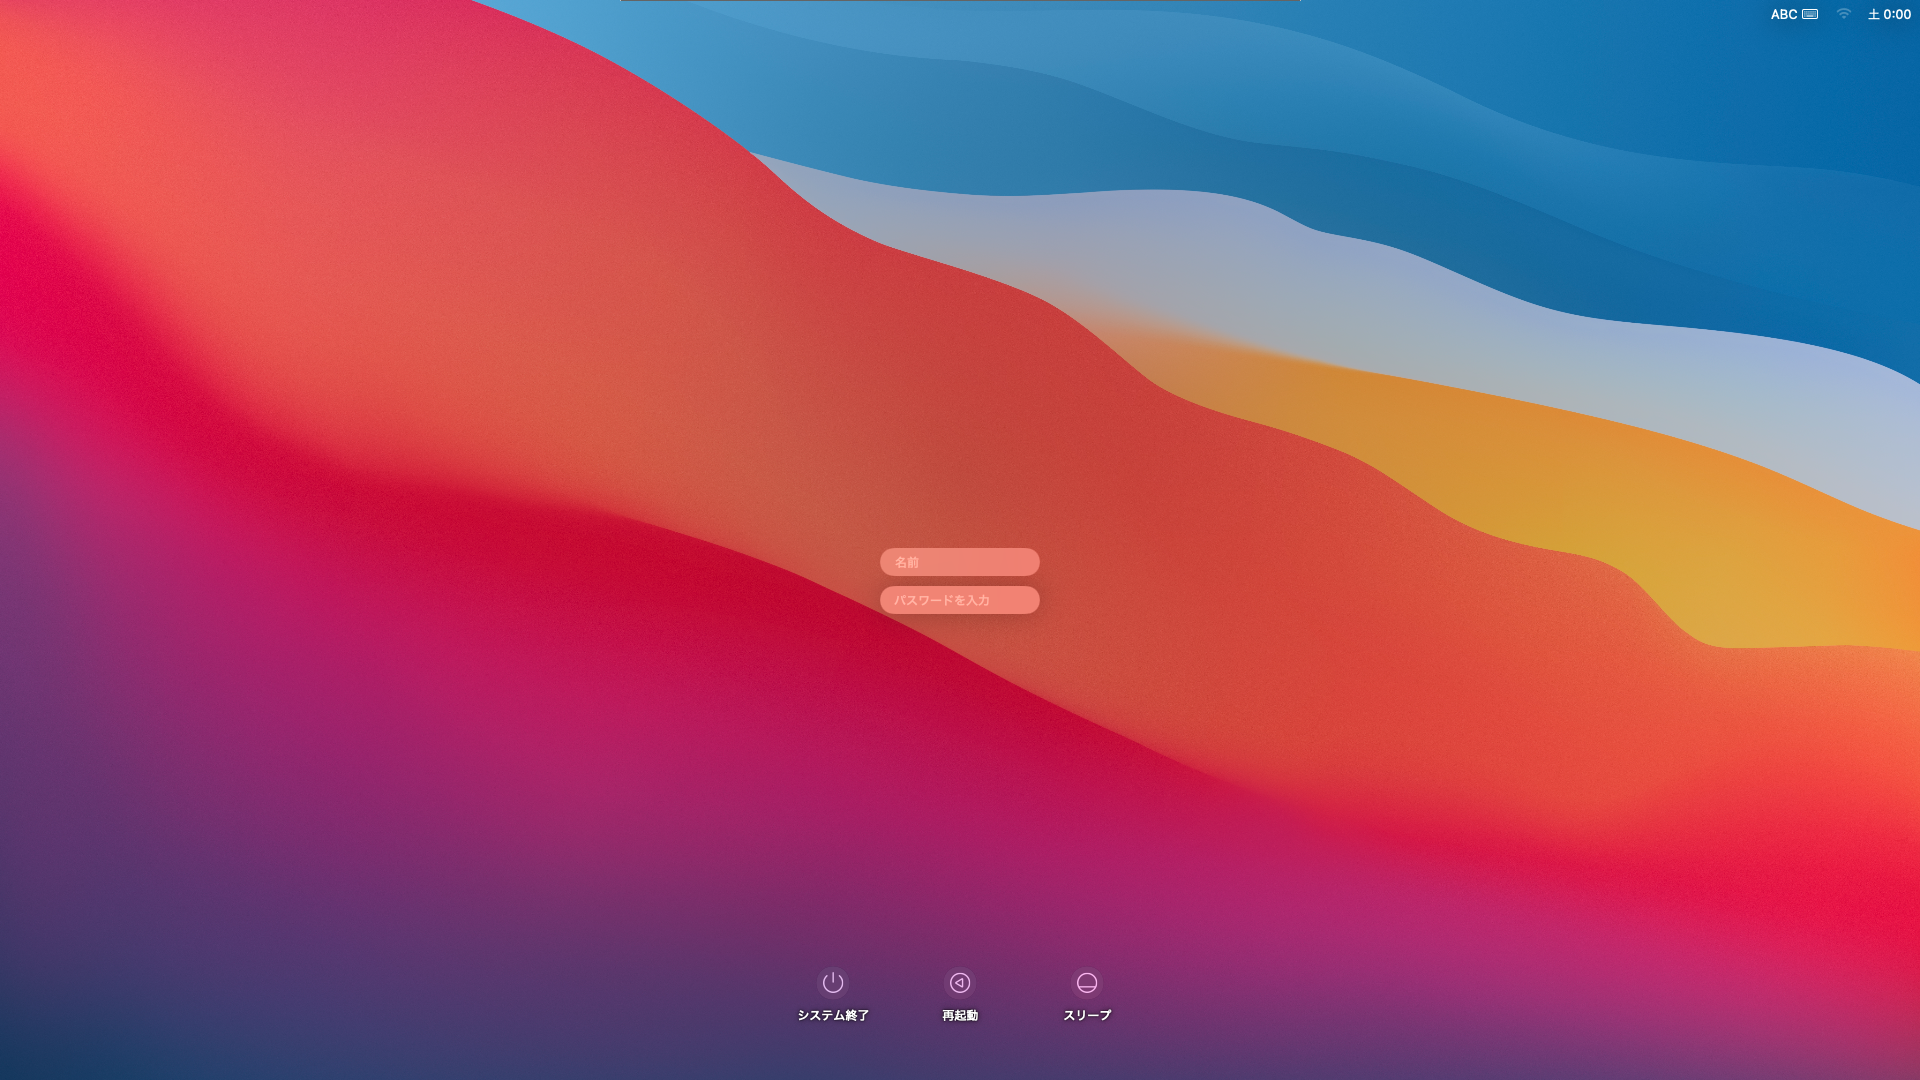
\includegraphics[height=7.5cm]{fig/MacLogin.png}
\end{figure}

初回ログイン時のみ,初期設定の画面が現れます.
\begin{enumerate}
  \item アクセシビリティ:「今はしない」
  \item データとプライバシー:「続ける」
  \item Siri: チェックボックスを外して「続ける」
  \item 外観モードを選択: お好みでどうぞ(後で変更できます)
\end{enumerate}

しばらくすると,デスクトップ画面が現れます.
\begin{figure}[H]
  \centering
  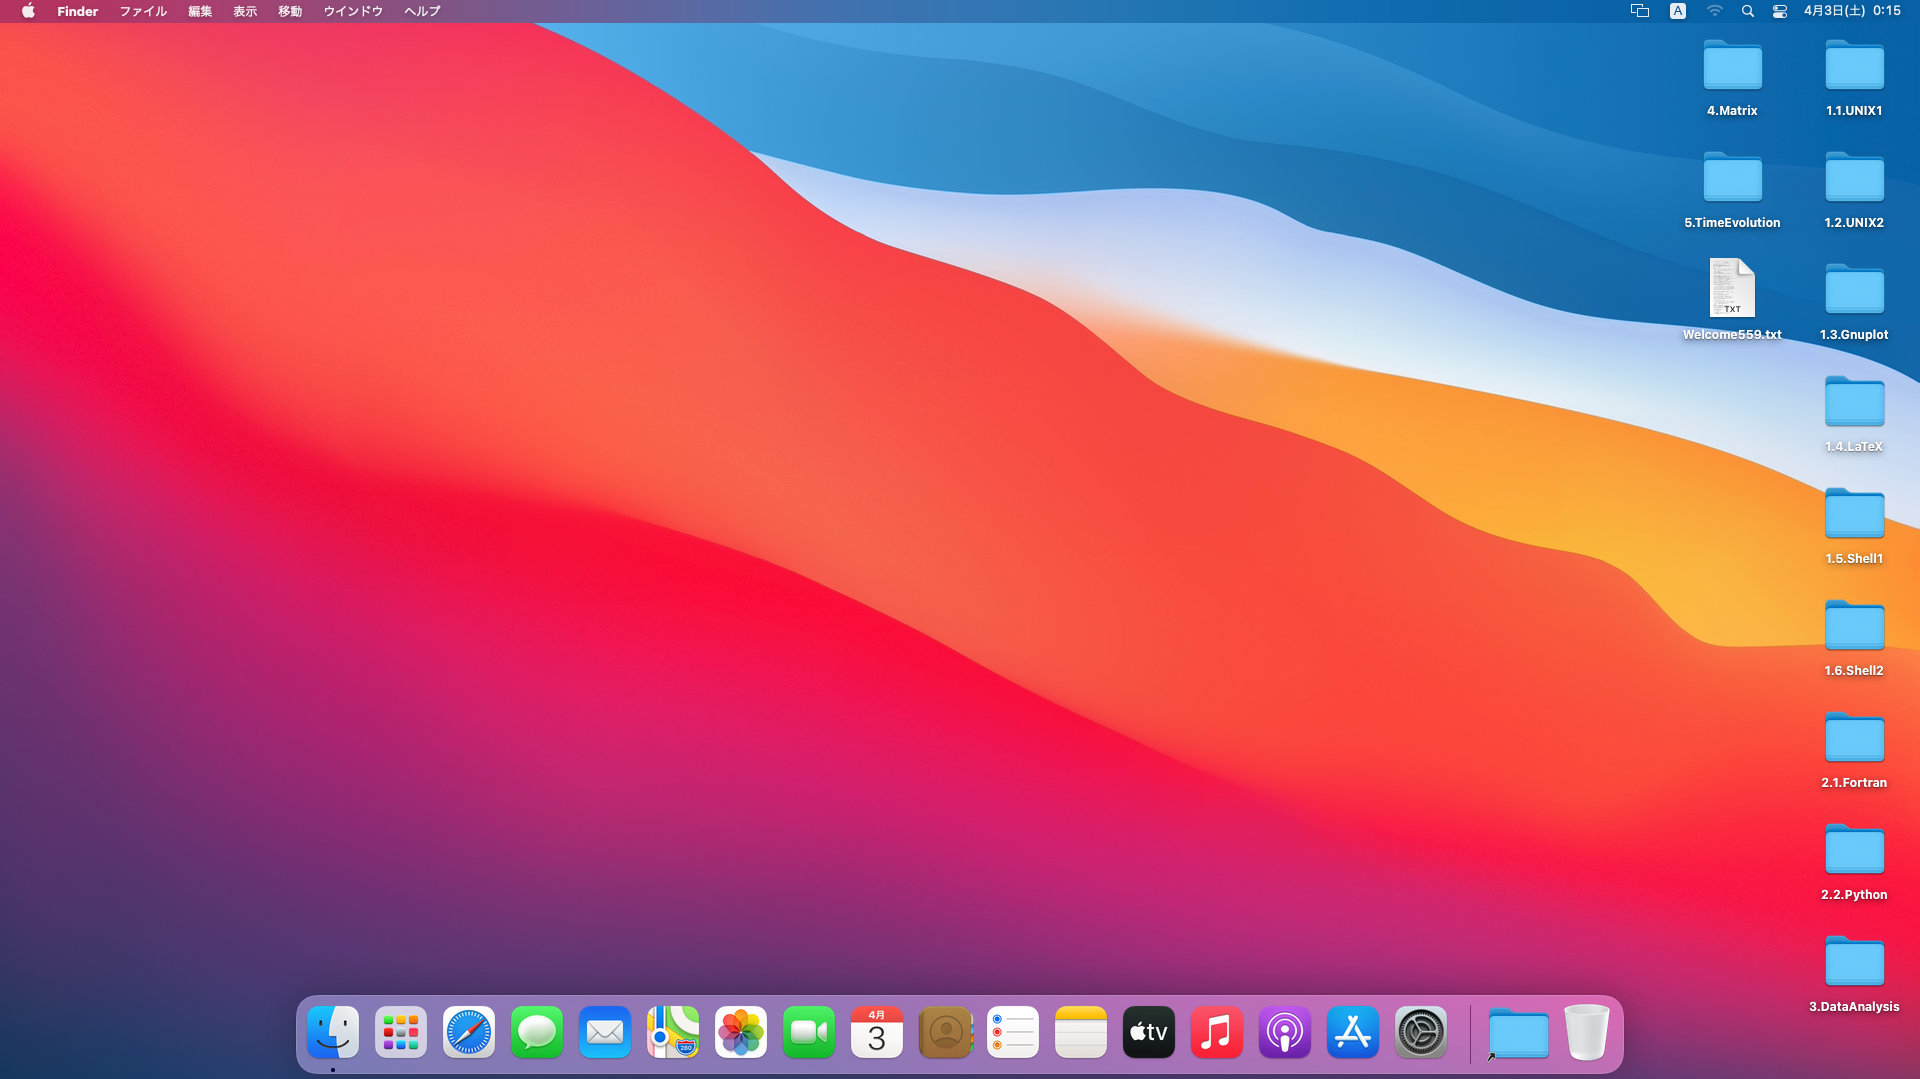
\includegraphics[height=7.5cm]{fig/MacDesktop.png}
\end{figure}

Macのデスクトップには,演習の各項目のディレクトリ(フォルダ)があります.
演習の課題などのファイルを置く場所として,ご自由にお使いください.

\subsection{ターミナル}
 CUI の操作はターミナルウィンドウとよばれるウィンドウの中で行われます.
 無事にログインできたら,ターミナルウィンドウを起動してみましょう. 

% ターミナルは以下のように起動します.
% \begin{center}
%   \begin{tabular}{ll}
%   {\bf xterm}\ $\rightarrow$ & Shift\ +\ Alt\ + x \\
%   {\bf kterm}\ $\rightarrow$ & Shift\ +\ Alt\ + k 
%   \end{tabular}
% \end{center}
% {\bf xterm}も{\bf kterm}も,どちらもターミナルの一種です.今回はとりあえず好きな方を使ってください.

Launchpadをクリックします.
\begin{figure}[H]
  \centering
  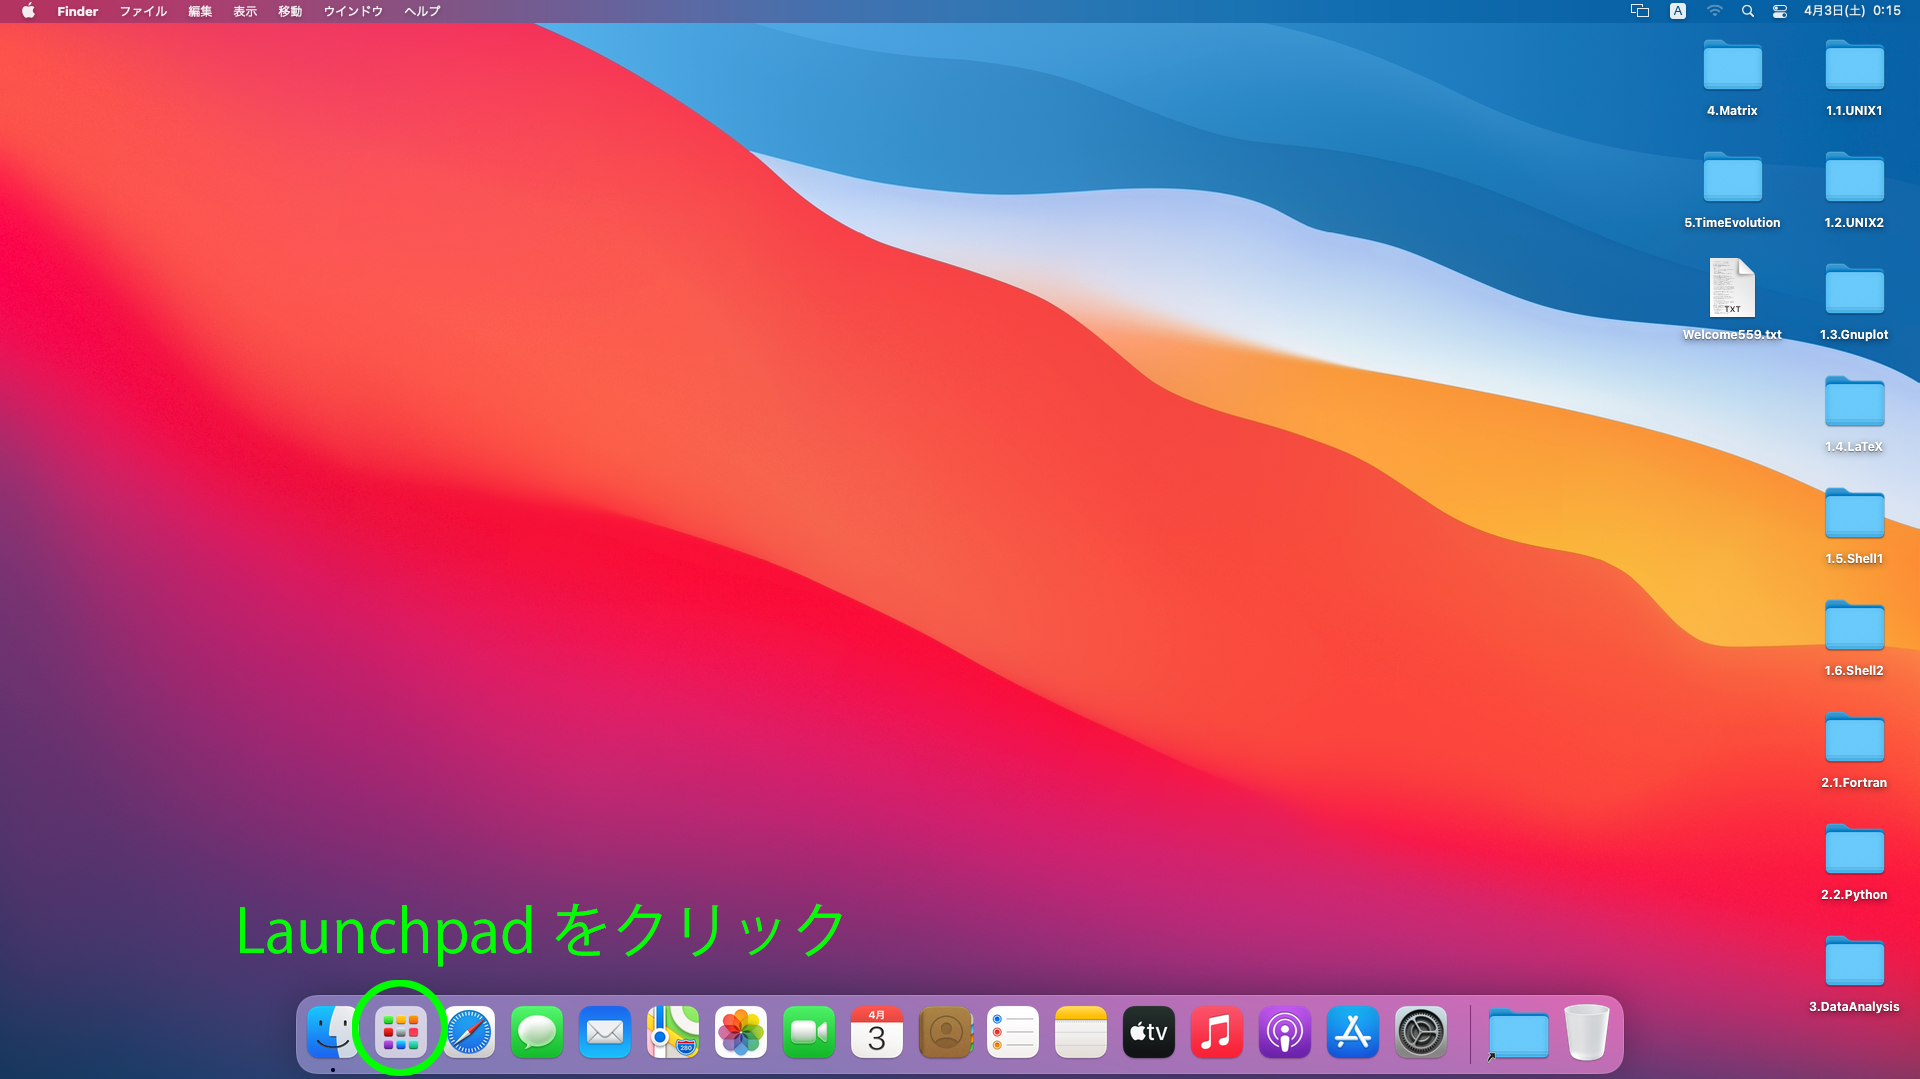
\includegraphics[height=7.5cm,pagebox=cropbox,clip]{fig/MacDesktopClickLaunchpad.png}
\end{figure}

\newpage
その他をクリックします.
\begin{figure}[H]
  \centering
  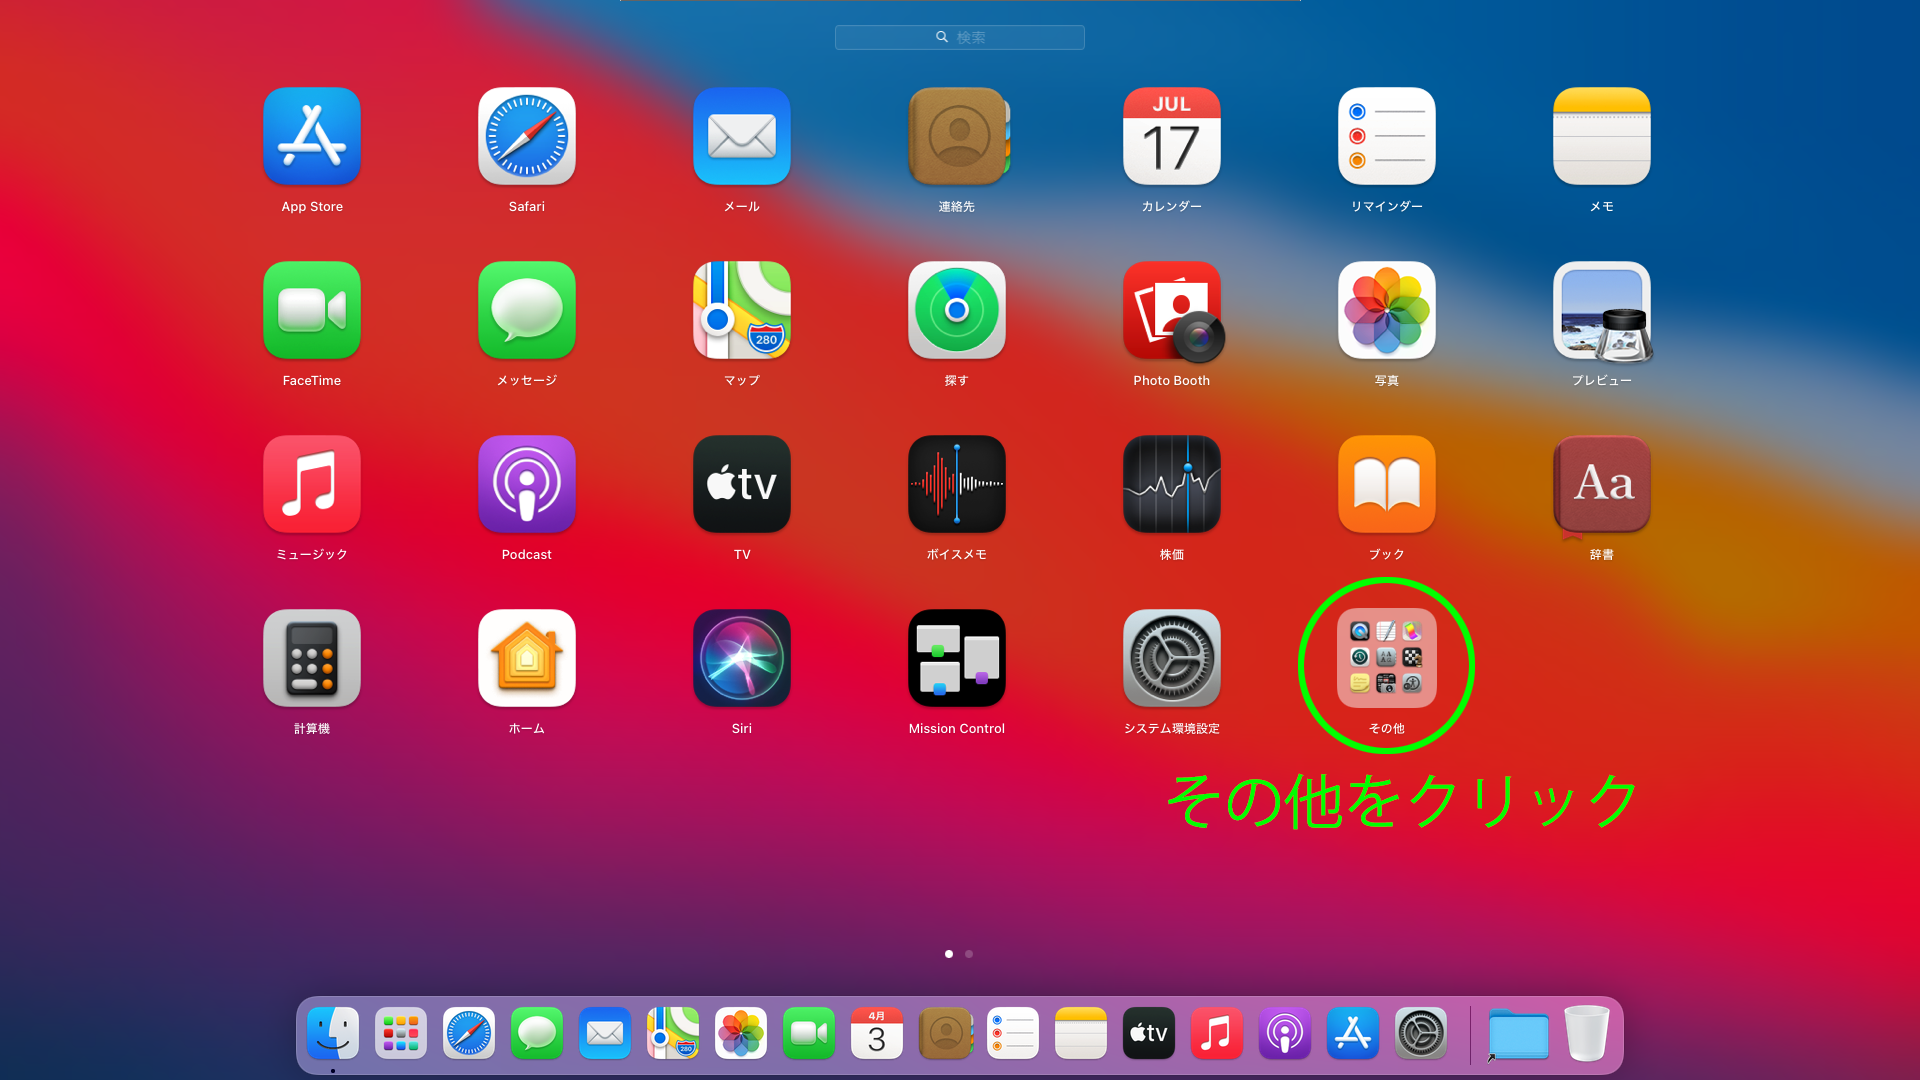
\includegraphics[height=7.5cm]{fig/MacLaunchpadClickOther.png}
\end{figure}

ターミナルをクリックします.
\begin{figure}[H]
  \centering
  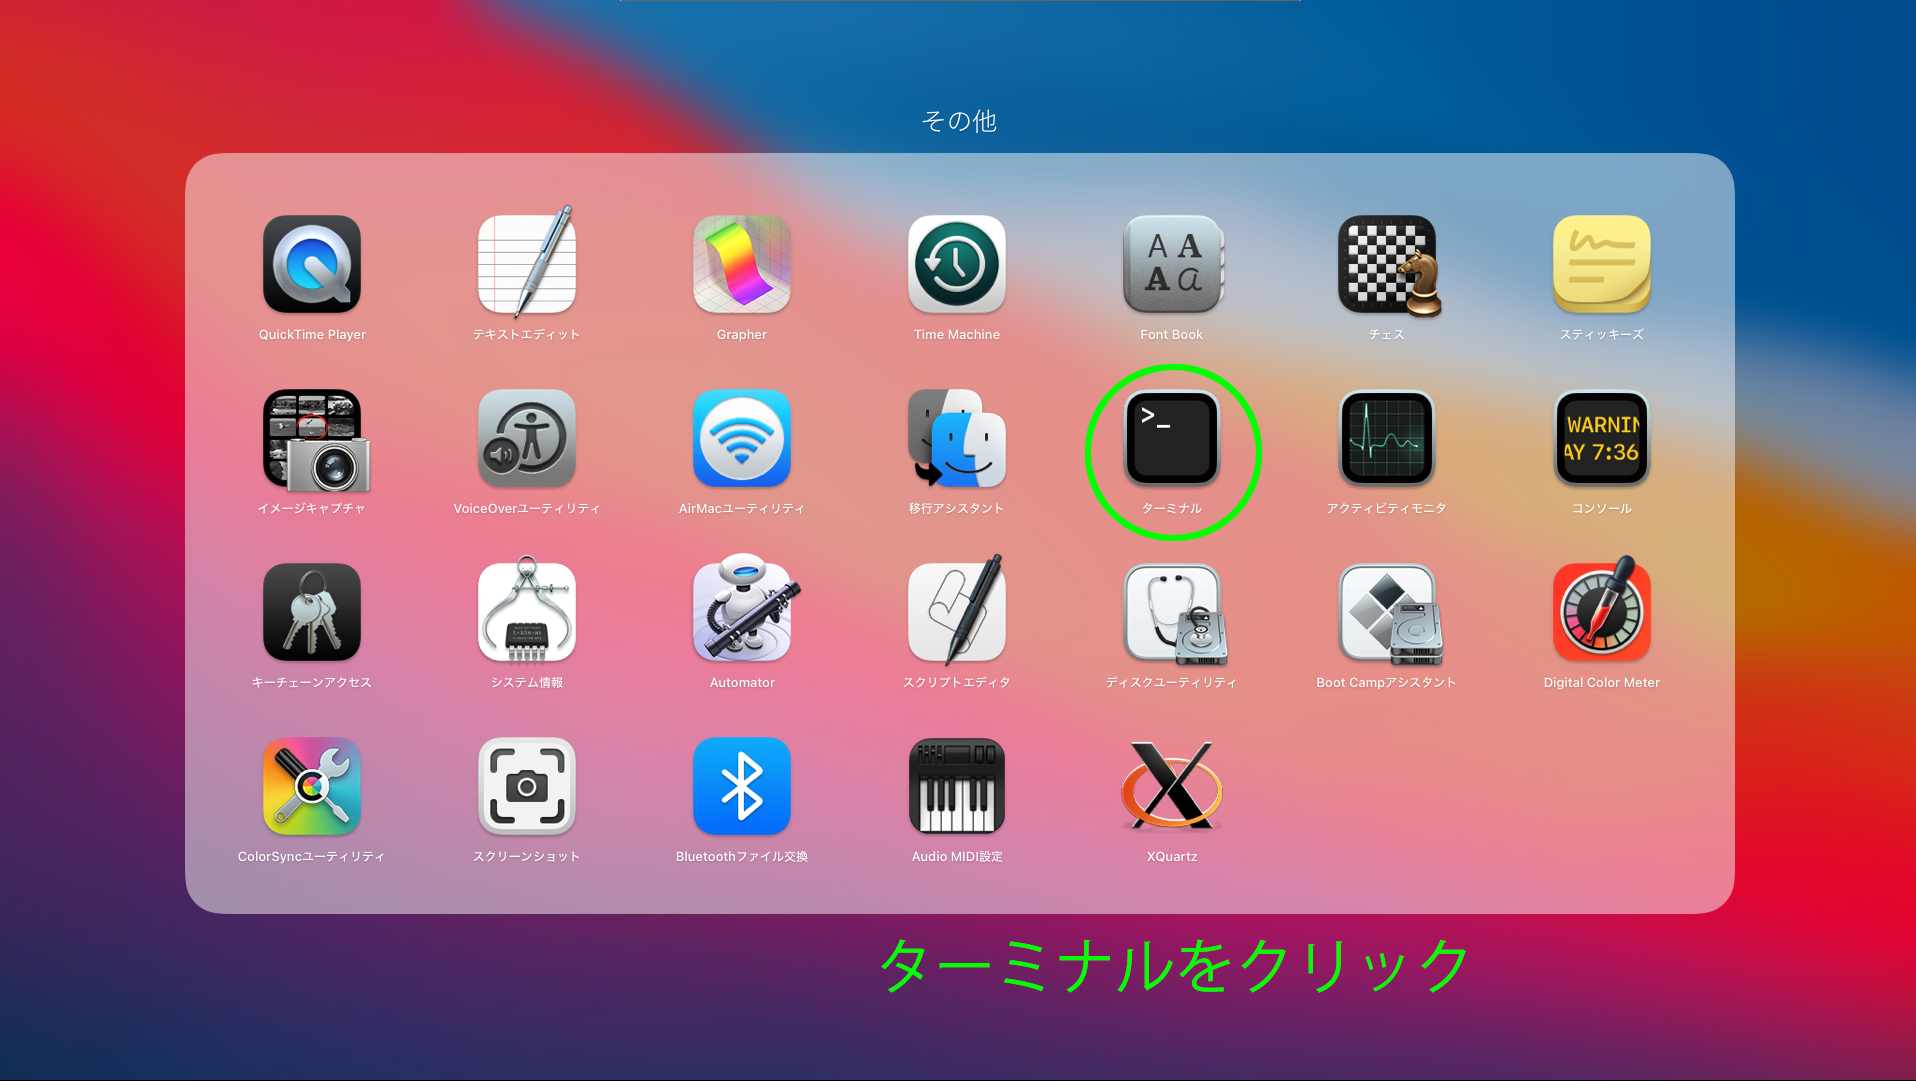
\includegraphics[height=7.5cm]{fig/MacLaunchpadOtherClickTerminal.png}
\end{figure}

\newpage
ターミナルが起動します.
\begin{figure}[H]
  \centering
  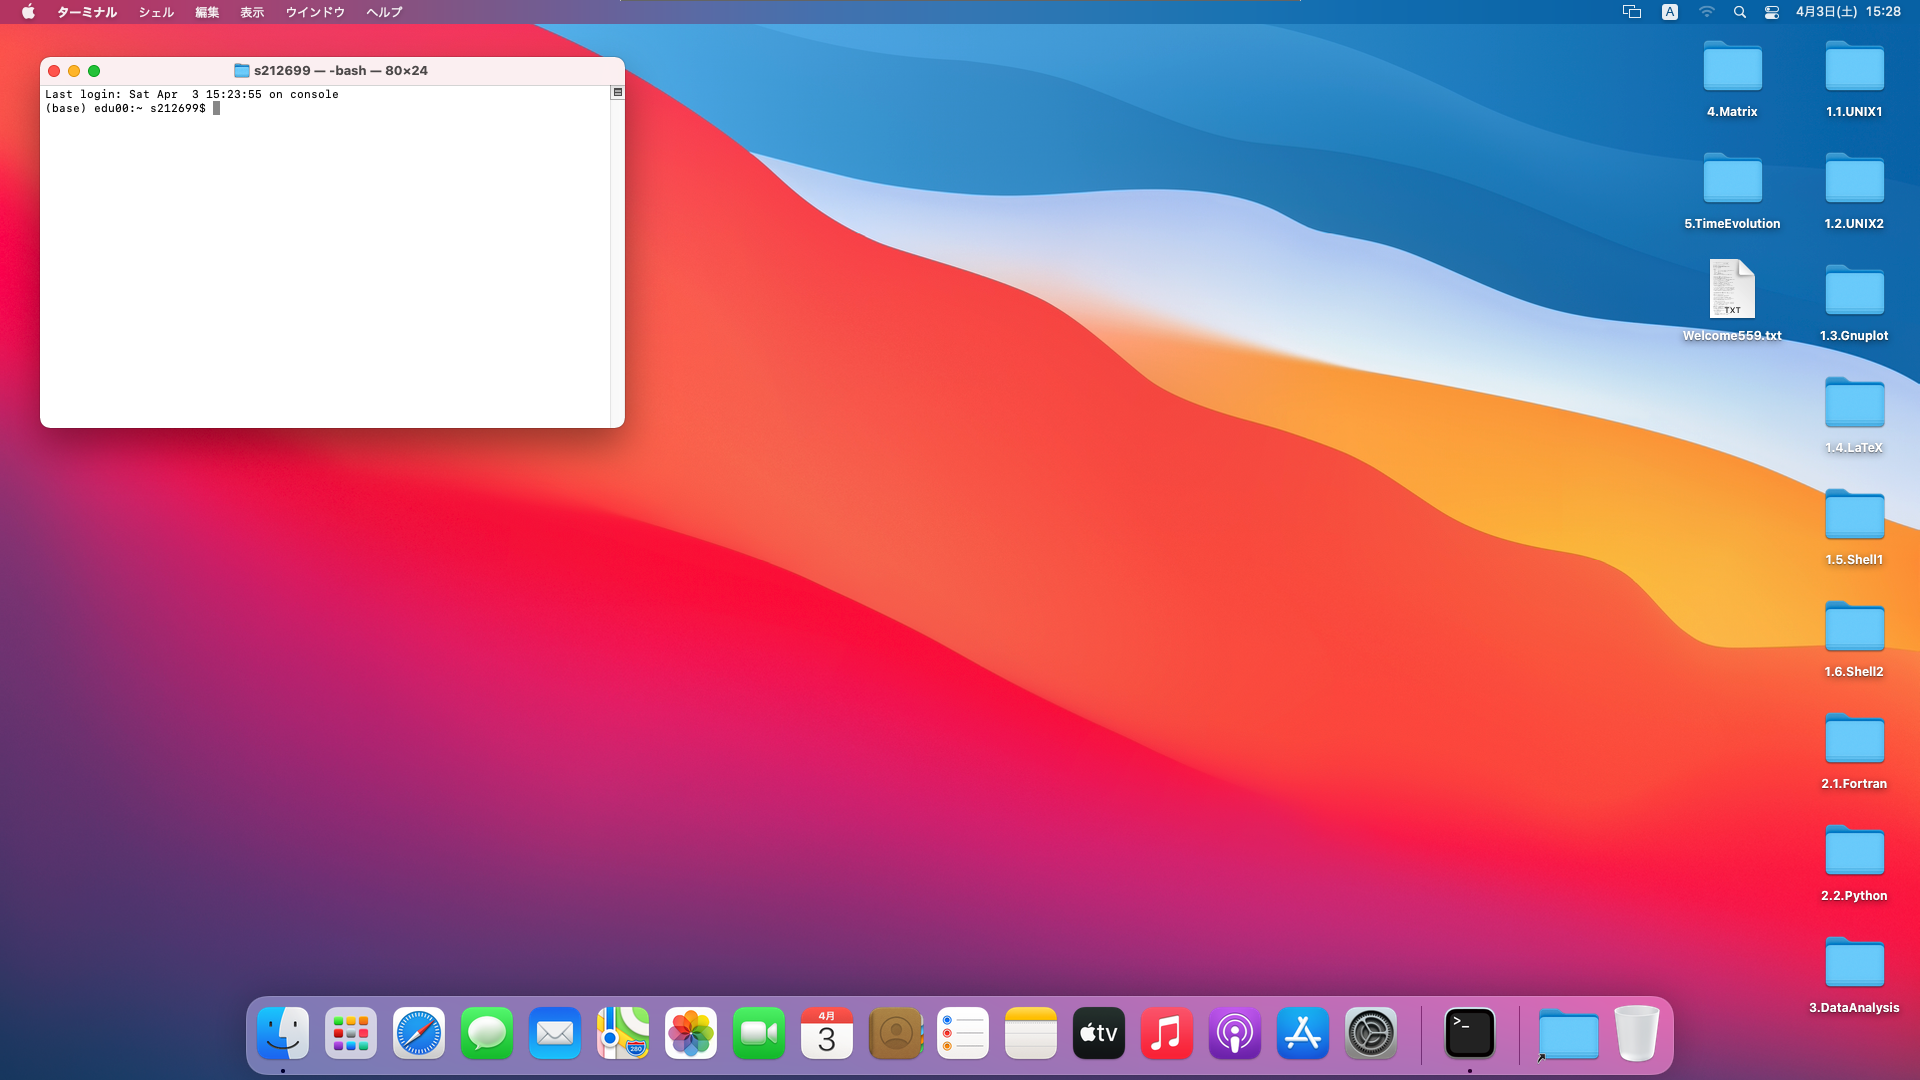
\includegraphics[height=7.5cm]{fig/MacTerminal.png}
\end{figure}

試しに\verb| ls Desktop |と入力してEnterキーを押してみましょう.
\begin{figure}[H]
  \centering
  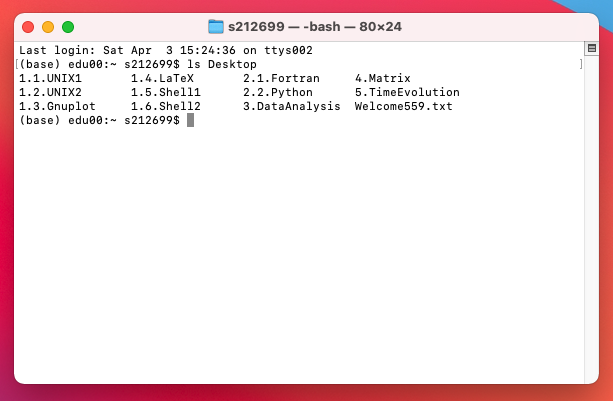
\includegraphics[height=7.5cm]{fig/MacTerminallsDesktop2.png}
\end{figure}
デスクトップにあるファイルやディレクトリの名前が表示されましたね.

\newpage
次に\verb| open -a safari |と入力してEnterキーを押してみましょう.\footnote{openコマンドはmacOS独自コマンドです.}
\begin{figure}[H]
  \centering
  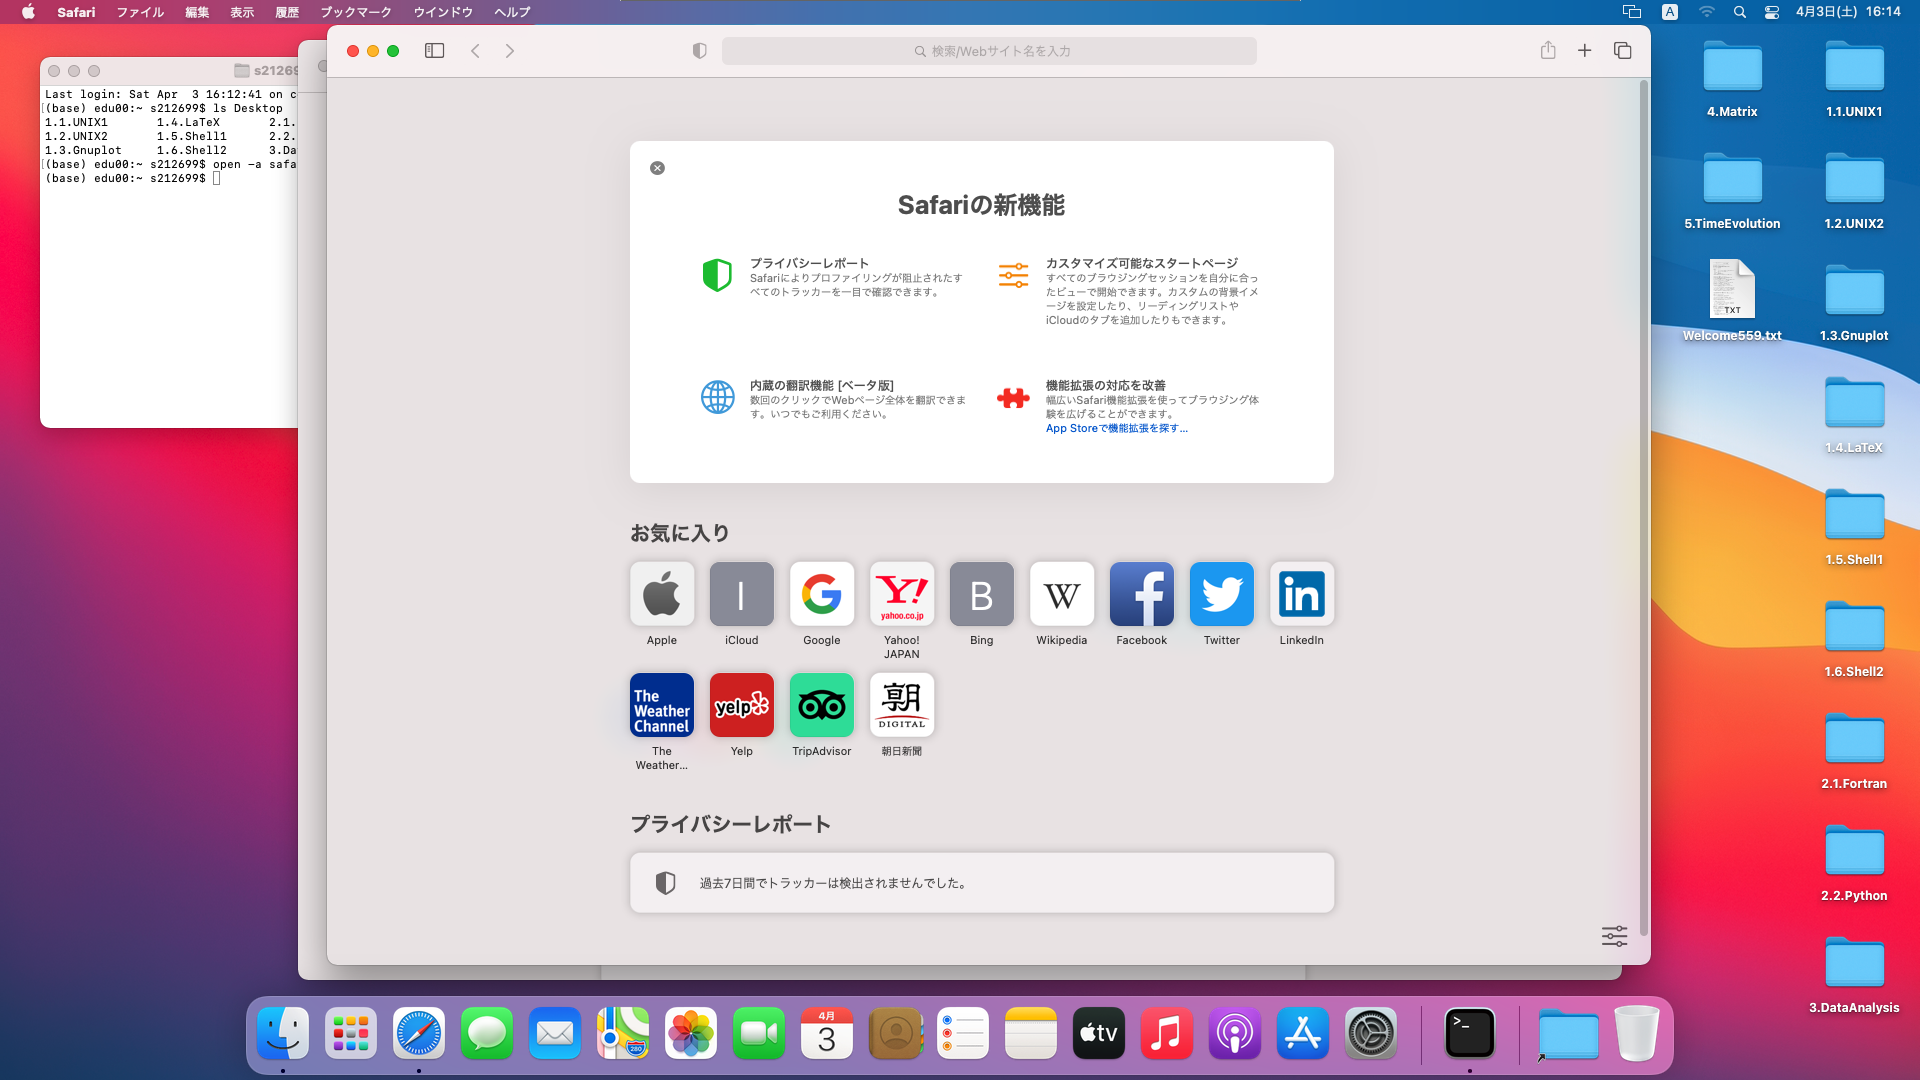
\includegraphics[height=7.5cm]{fig/MacTerminalOpenSafari.png}
\end{figure}
Safariが起動しましたね.\verb| open -a firefox |と入力すればFirefoxが起動します.
もちろんSafariやFirefoxは,普通にDockやLaunchpadのアイコンをクリックしても起動します.\\

ターミナルを終了するときは\verb| exit |と入力してから,ウィンドウを閉じてください.\\

ターミナルはこのままでも使うことができますが,文字が見えにくいと思う場合は
次の手順で見た目を変更することができます.
\begin{figure}[H]
  \centering
  リンゴマークの右の「ターミナル」→「環境設定」→「プロファイル」\\
  \ \\
  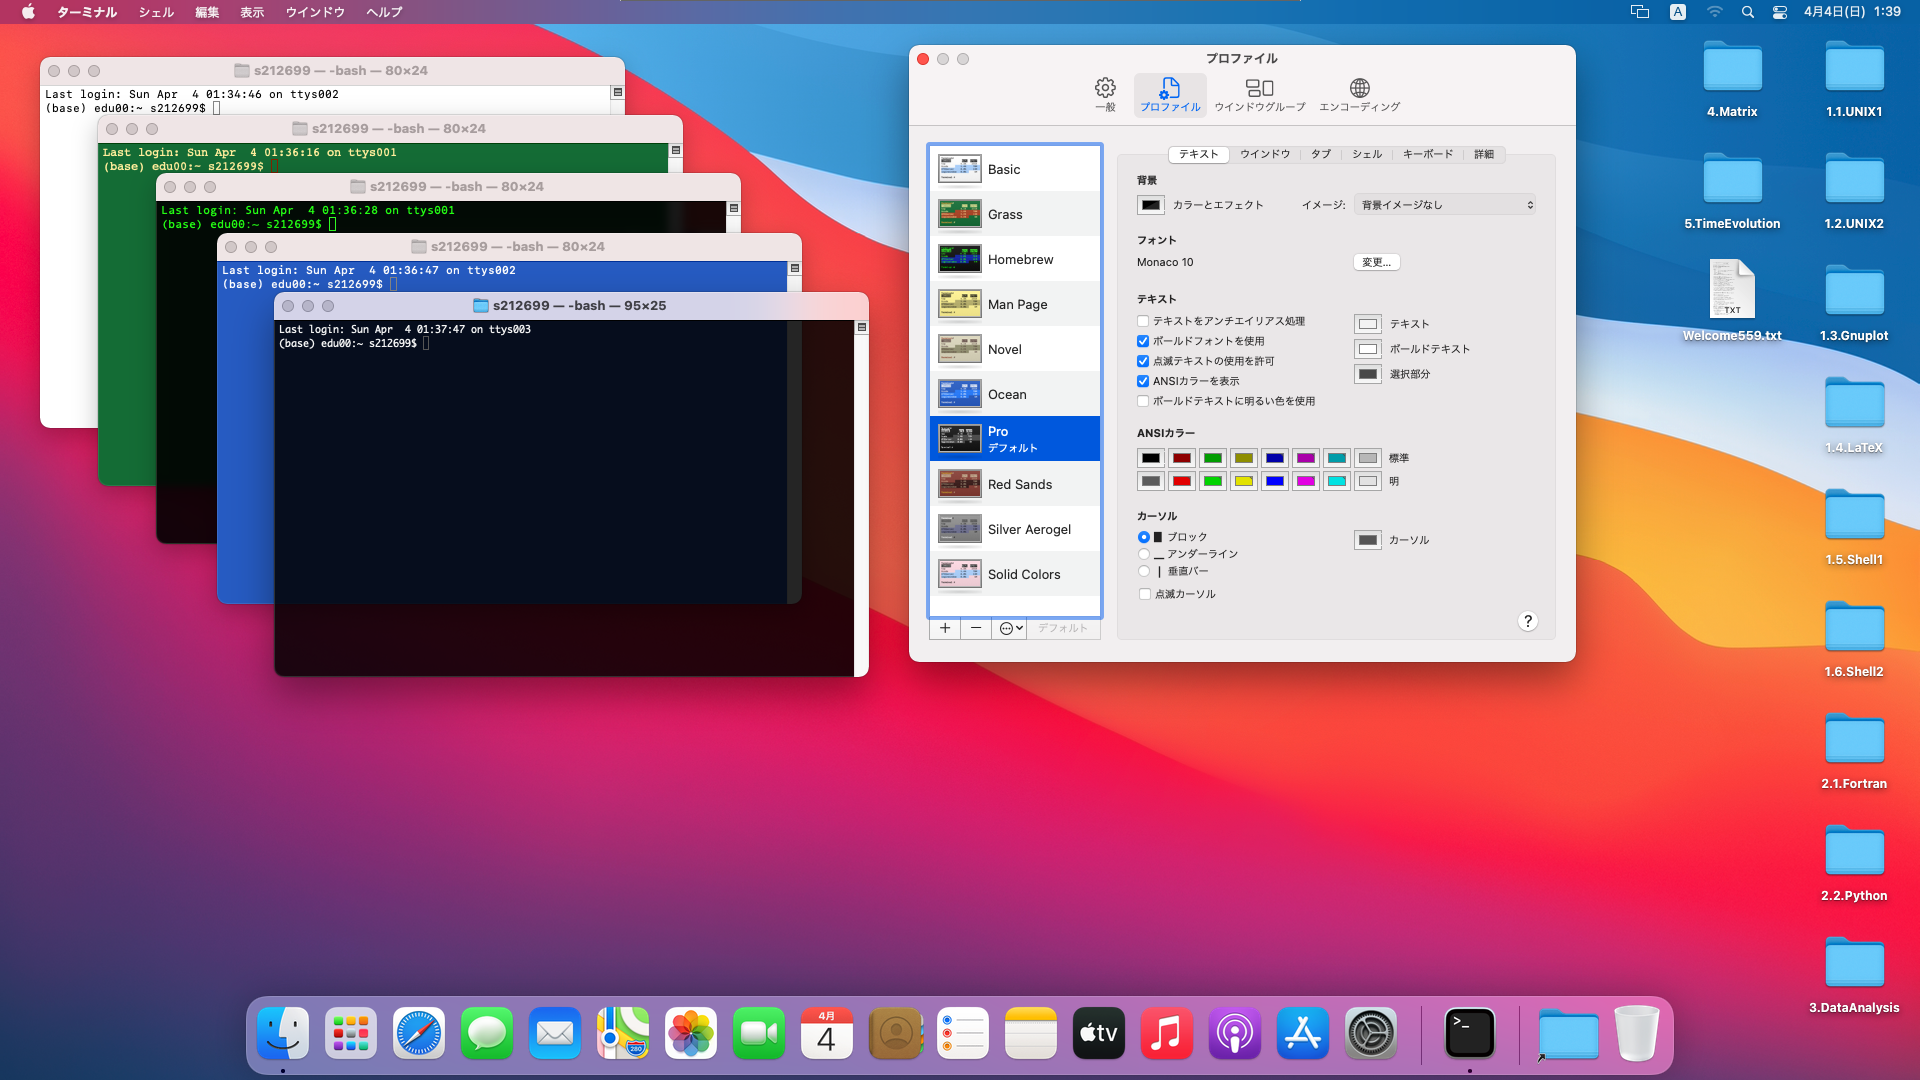
\includegraphics[height=7.5cm]{fig/MacTerminalSetting.png}
\end{figure}
左のプロファイルの一覧からお好みのものを選んでください.フォントや文字サイズも見やすいものに変えましょう.

今後は,このターミナル上でコマンドを入力することによって多くの作業を行うことになります.
また,次回以降「ターミナル」とか「シェル」とかいう言葉はこれを指していると考えて下さい.\\ 
%  また,このターミナルで peep_TA & と打ち込んでリターンを押すと TA の端末画面を
%  のぞき見することができます.説明の都合で TA の画面を皆さんに見ていただきたい
%  ときがあるかも知れませんが,そのときは peep_TA を実行してみて下さい.

% \subsection{Firefox \& ECCS クラウドメール}
% 次に Firefox を起動しましょう.FirefoxはInternet ExplorerとかSafariとかGoogle Chromeとかと同じWeb Browserの一つです.\\
% ターミナルで\\
% \quad \quad \quad {\bf{\$ firefox \&}}\\
% と入力してください.(\$\ はプロンプトと呼ばれるもの.
% 実際に入力するのは「firefox \&」の部分.以下同様).

以上でログイン方法およびターミナル,Webブラウザの起動方法を学びましたね.

今後,講義の最中にわからないことがあった時はやみくもにTAに質問するのではなく,ソフトウェアの使い方やエラーの内容をどんどん検索して{\bf 解決策を自力で探す}ことに慣れてください.
計算機演習に限らず,日常のあらゆるトラブルに対して{\bf 「検索力」}はあなたの助けになってくれるでしょう.

とはいえ,慣れないうちは自力でどうしても解決できない問題にも多々直面するものです.そうした時には近くのTAに「何が分からないのか(あるいは何も分からないのか)」要点を絞って質問するようにして,より効率的に問題解決へアプローチしましょう.

\subsection{edu(Mac)のアプリケーション}
Launchpadで,下にある2番目の点(・)をクリックします.
\begin{figure}[H]
  \centering
  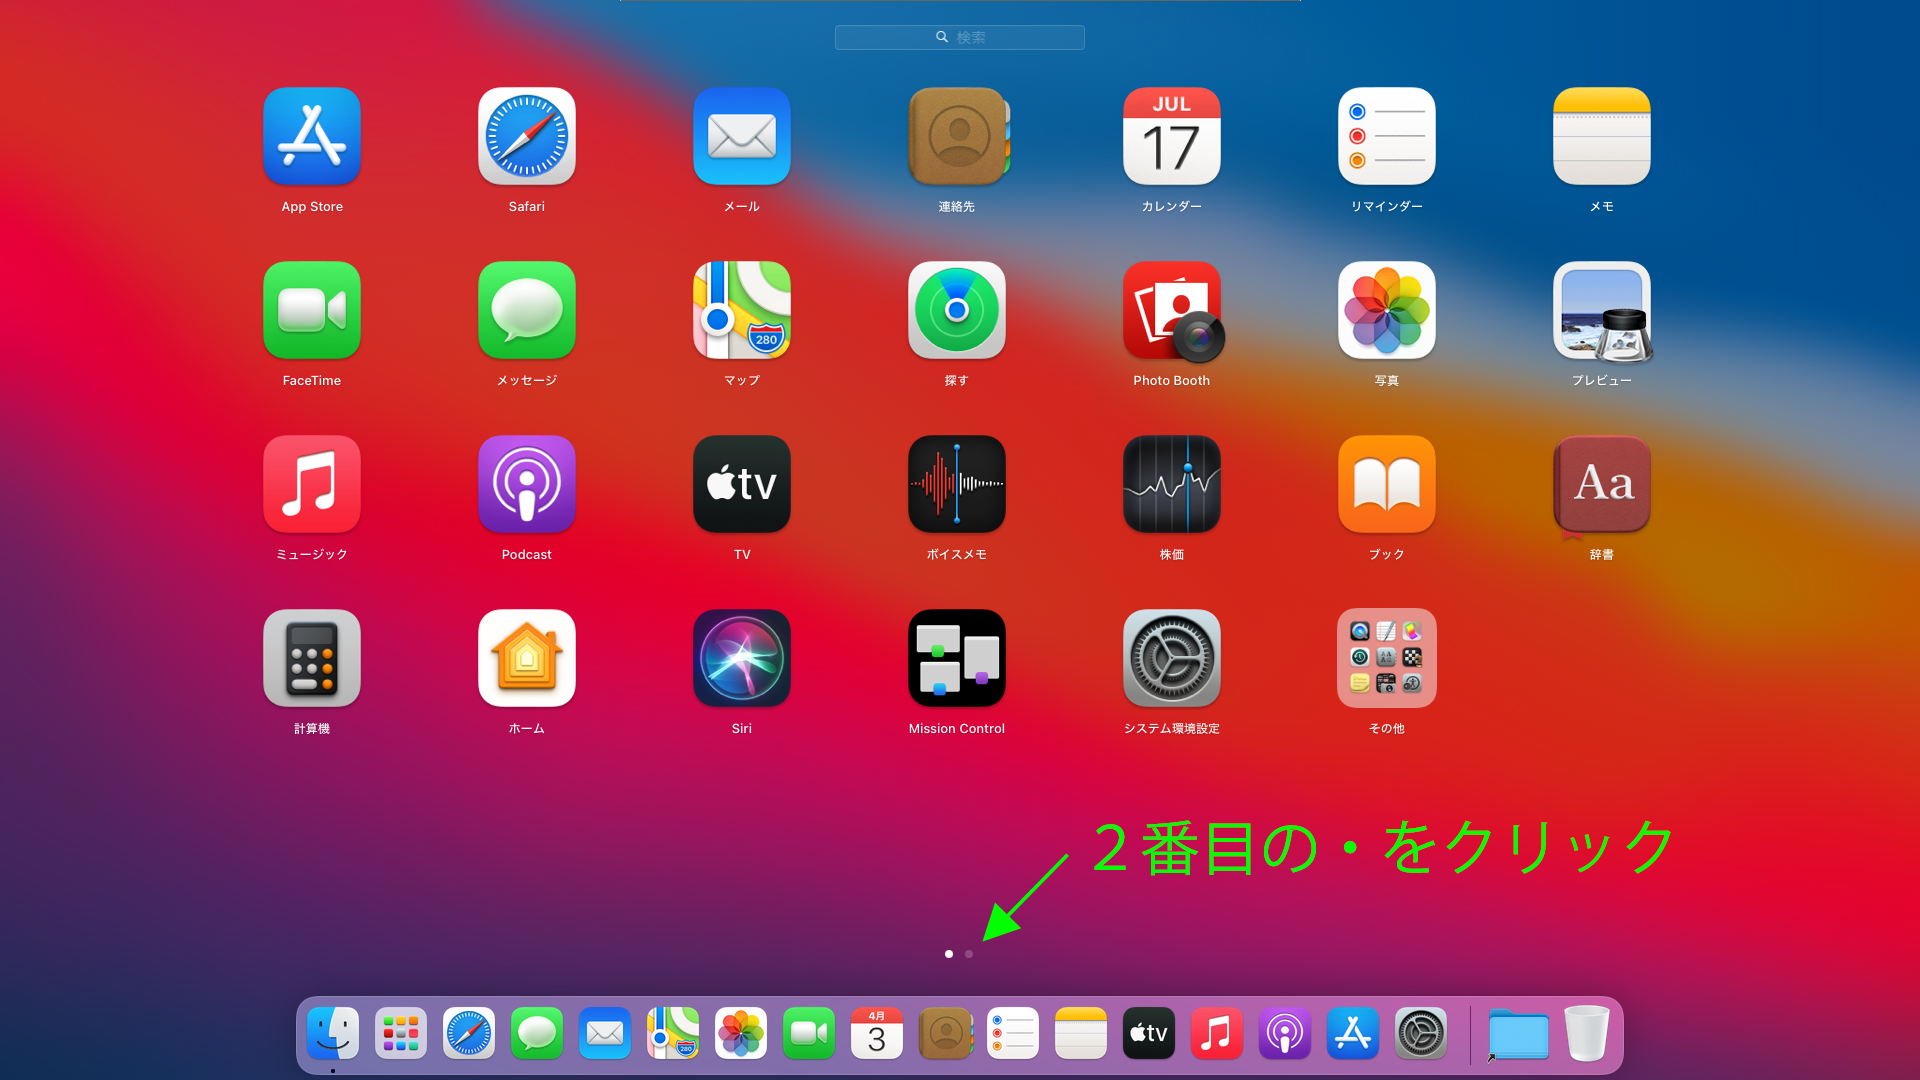
\includegraphics[height=7.5cm]{fig/MacLaunchpadClick2.png}
\end{figure}

\newpage
するとedu(Mac)にインストールされてあるアプリケーションが表示されます.
\begin{figure}[H]
  \centering
  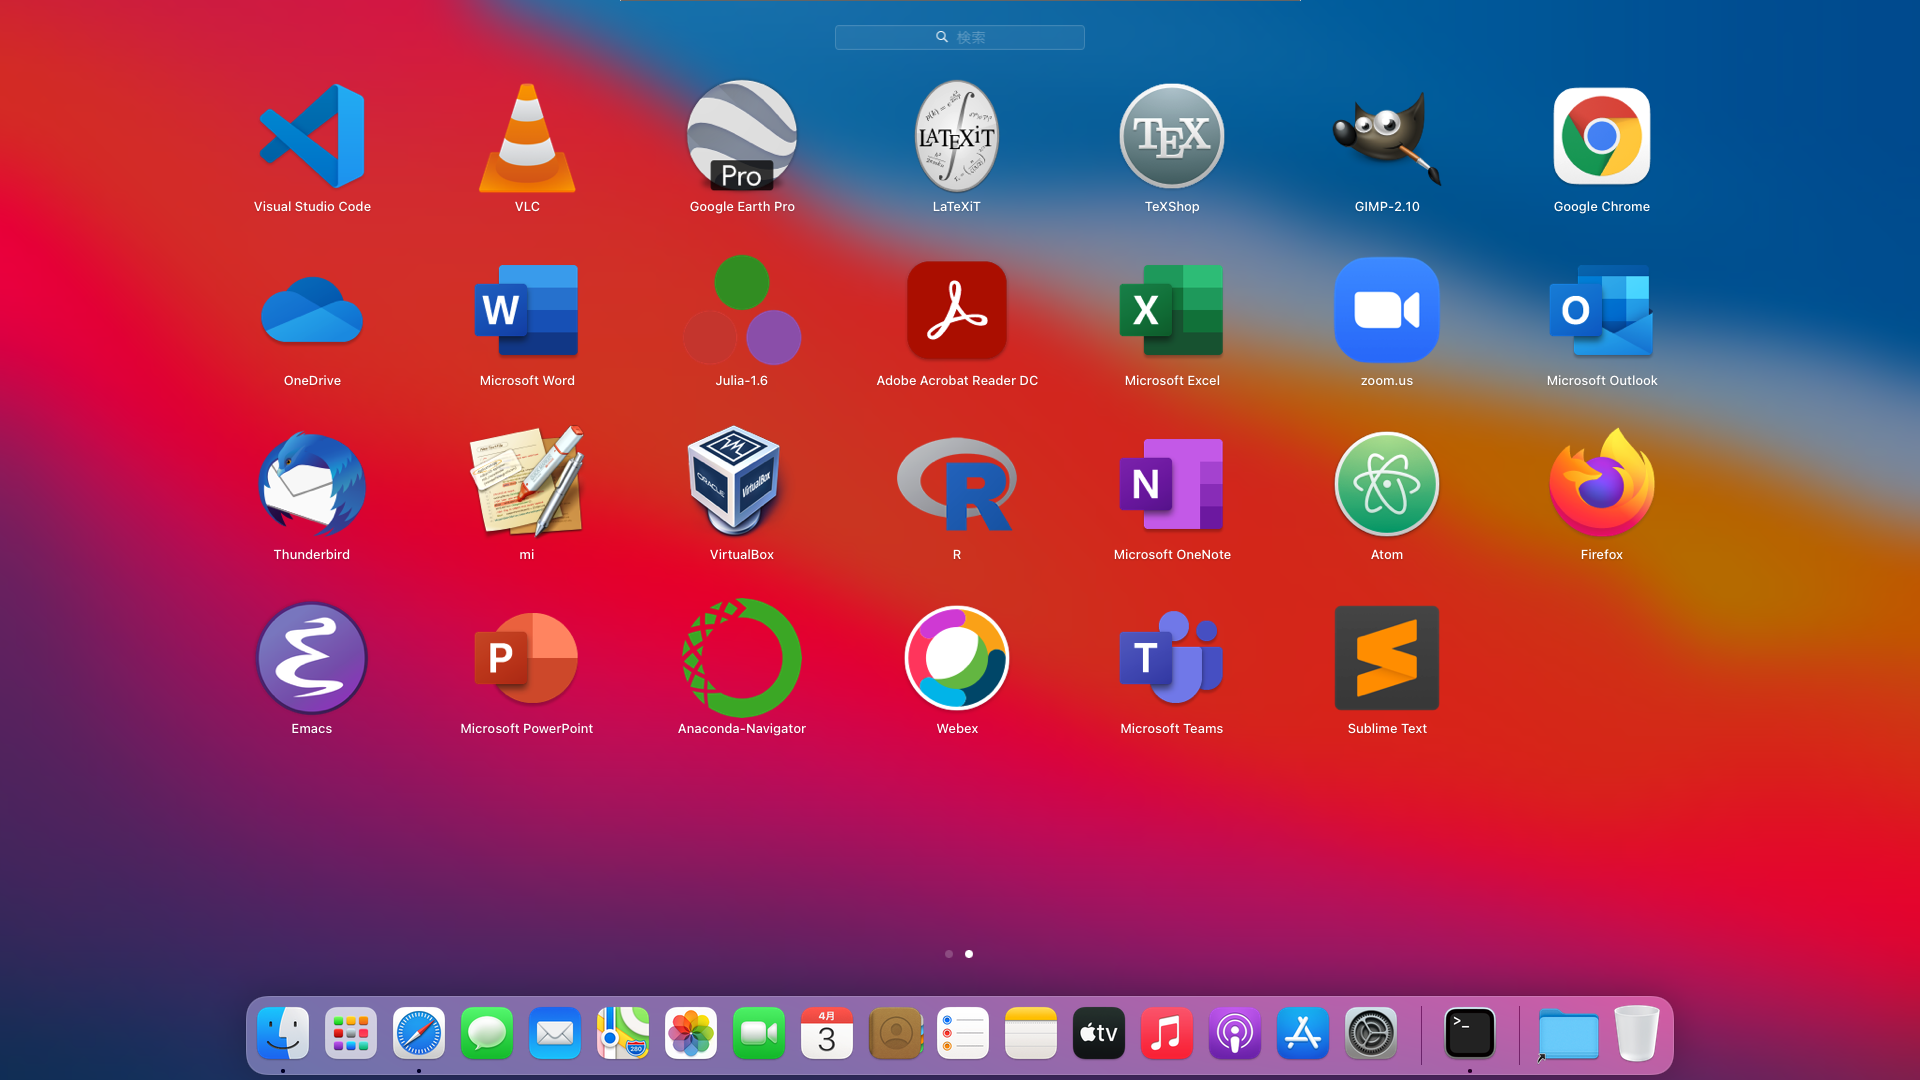
\includegraphics[height=7.5cm]{fig/MacLaunchpad2.png}
\end{figure}

簡単に説明すると
\begin{itemize}
  \item テキストエディタ: テキストファイルやソースコードを編集するためのアプリケーション\\
    Emacs, Visual Studio Code, Atom, mi, SublimeText
  \item \TeX ユーティリティ\\
    LaTeXiT, TeXShop
  \item プログラミング言語開発環境\\
    Anaconda(Python), R, Julia
  \item ウェブブラウザ\\
    Safari, Firefox, Google Chrome
  \item メールソフト\\
    Thunderbird
  \item Microsoft Office\\
    Excel, Word, PowerPoint, Outlook, OneNote, OneDrive\\
    ※各自の大学アカウント(共通IDの数字10桁@utac.u-tokyo.ac.jp)でサインインして利用してください
  \item Web会議システム(マイクとカメラは各自で用意してください)\\
    Zoom, Teams, WebEx
  \item その他\\
    Google Earth, Acrobat Reader, VLC(動画再生), Gimp(画像編集)など
\end{itemize}
といったアプリケーションがインストールされています.
使い方やわからないことは検索したりTAに質問したりしながら,どんどん使っていきましょう!

\newpage
\section{ECCS クラウドメール・Thunderbird・Slack}
\subsection{ECCS クラウドメール}
\subsubsection{メールアカウント}
さて,皆さんは教育用計算機システム({\bf ECCS})のメールアドレスを使用することが
できます.
地物学科では地惑事務室からの重要な連絡事項や講義の課題レポートの提出などはこのメールアドレスを通してやり取りすることが多くなりますので,ECCSアドレスの設定がしっかり機能しているかおきましょう.

まず,SafariかFirefoxで
\begin{center}
 \href{https://www.ecc.u-tokyo.ac.jp/announcement/2016/04/01_2159.html}{https://www.ecc.u-tokyo.ac.jp/announcement/2016/04/01\_2159.html}
\end{center}
へアクセスしてください.

ECCS クラウドメールにログインできるか確認しましょう.下図の赤枠内のリンクからアクセスしてください.
\begin{figure}[H]
  \begin{center}
     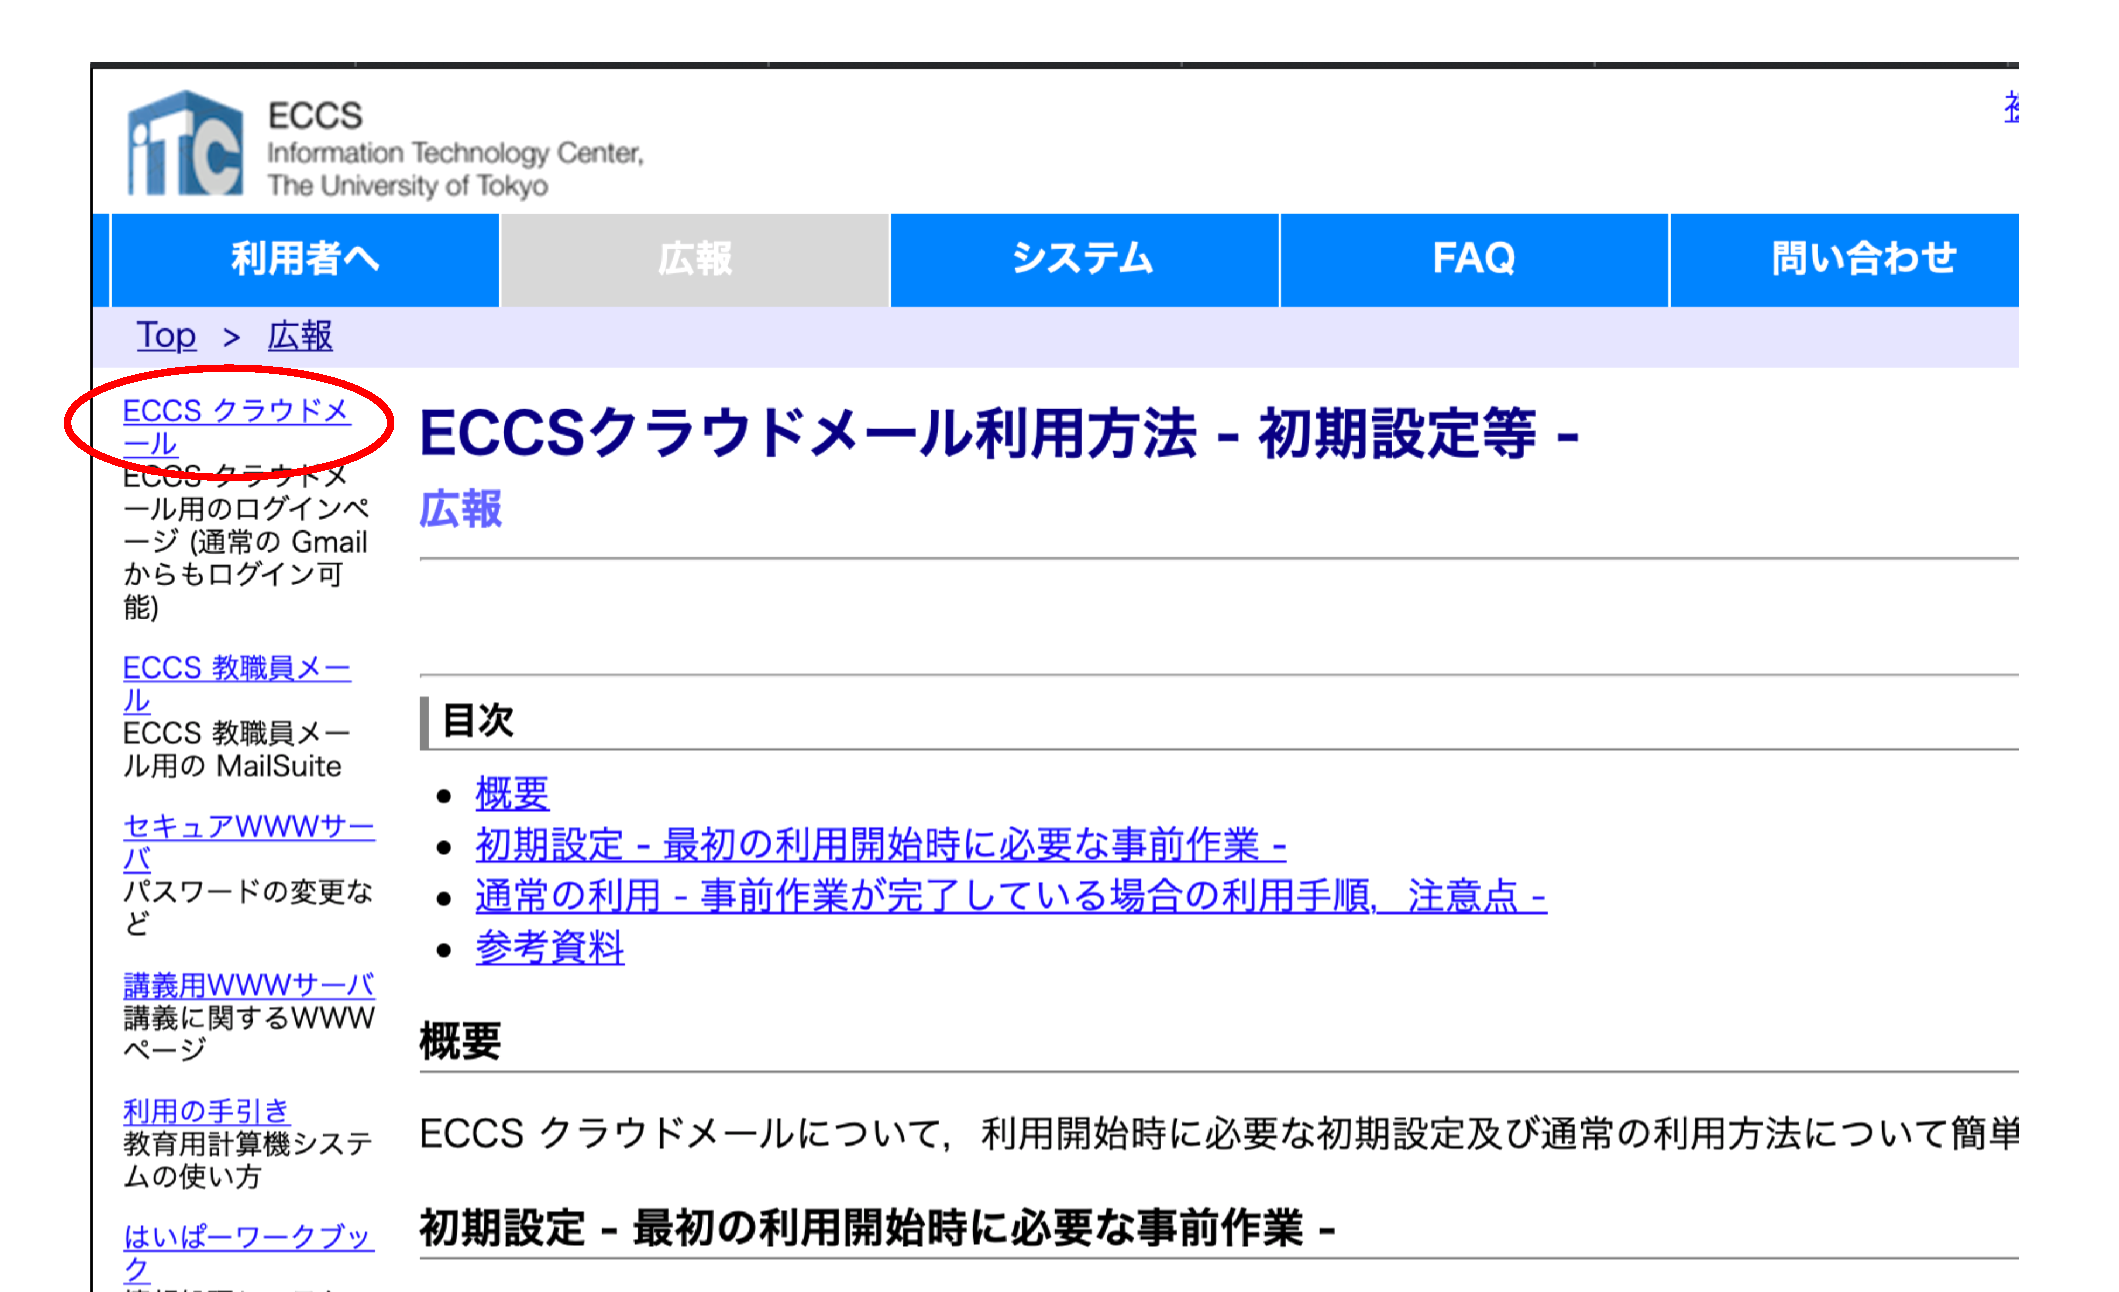
\includegraphics[width=150mm,pagebox=cropbox,clip]{fig/eccs.png}
  \end{center}
\end{figure}

ログインできない人や,そもそもECCSクラウドメールを設定していない人は,このページに従って設定しておきましょう.
\begin{center}
  % \href{https://utacm.adm.u-tokyo.ac.jp/webmtn/LoginServlet}{https://utacm.adm.u-tokyo.ac.jp/webmtn/LoginServlet}
  \href{https://www.ecc.u-tokyo.ac.jp/announcement/2016/04/01\_2159.html}{https://www.ecc.u-tokyo.ac.jp/announcement/2016/04/01\_2159.html}
\end{center}
% 2569278065 

UTokyoアカウント名は10桁の番号です.アカウント名やパスワードが分からない場合はTAにご相談ください.

\vspace{1em}

ログインできましたか?今後の演習はもちろん,事務からの重要なメールも基本的にはこのアドレスに届
 くので,こまめにメールをチェックしましょう.なお ECCS クラウドメールは Gmail アプリなどからもログイン可能です.ECCSのHPに詳しい説明がありますので,各自のスマートフォンやノートパソコンからこまめにメール確認できるようにしておきましょう.

\subsubsection{署名の作成}
せっかくログインできることを確認できたので,より実用的な設定を行っておきましょう.
例えば,毎回署名(送り主のプロフィールを記載したもの)を書くのは大変です.
作成するメールに自動的に署名が挿入されるよう,設定しましょう.

ログイン後の画面の右上の方に「歯車」のアイコンがあるのでこれをクリックし「設定」へ進みましょう.
画面遷移すると様々な設定項目が出てきますが\ 「署名」はページの後方にあります.下の図のように所属・名前など基本的な情報を載せるようにしておくと良いでしょう.海外の方と連絡を取ることが多い方は英語ver.も用意しておくのが吉です.

\begin{center}
  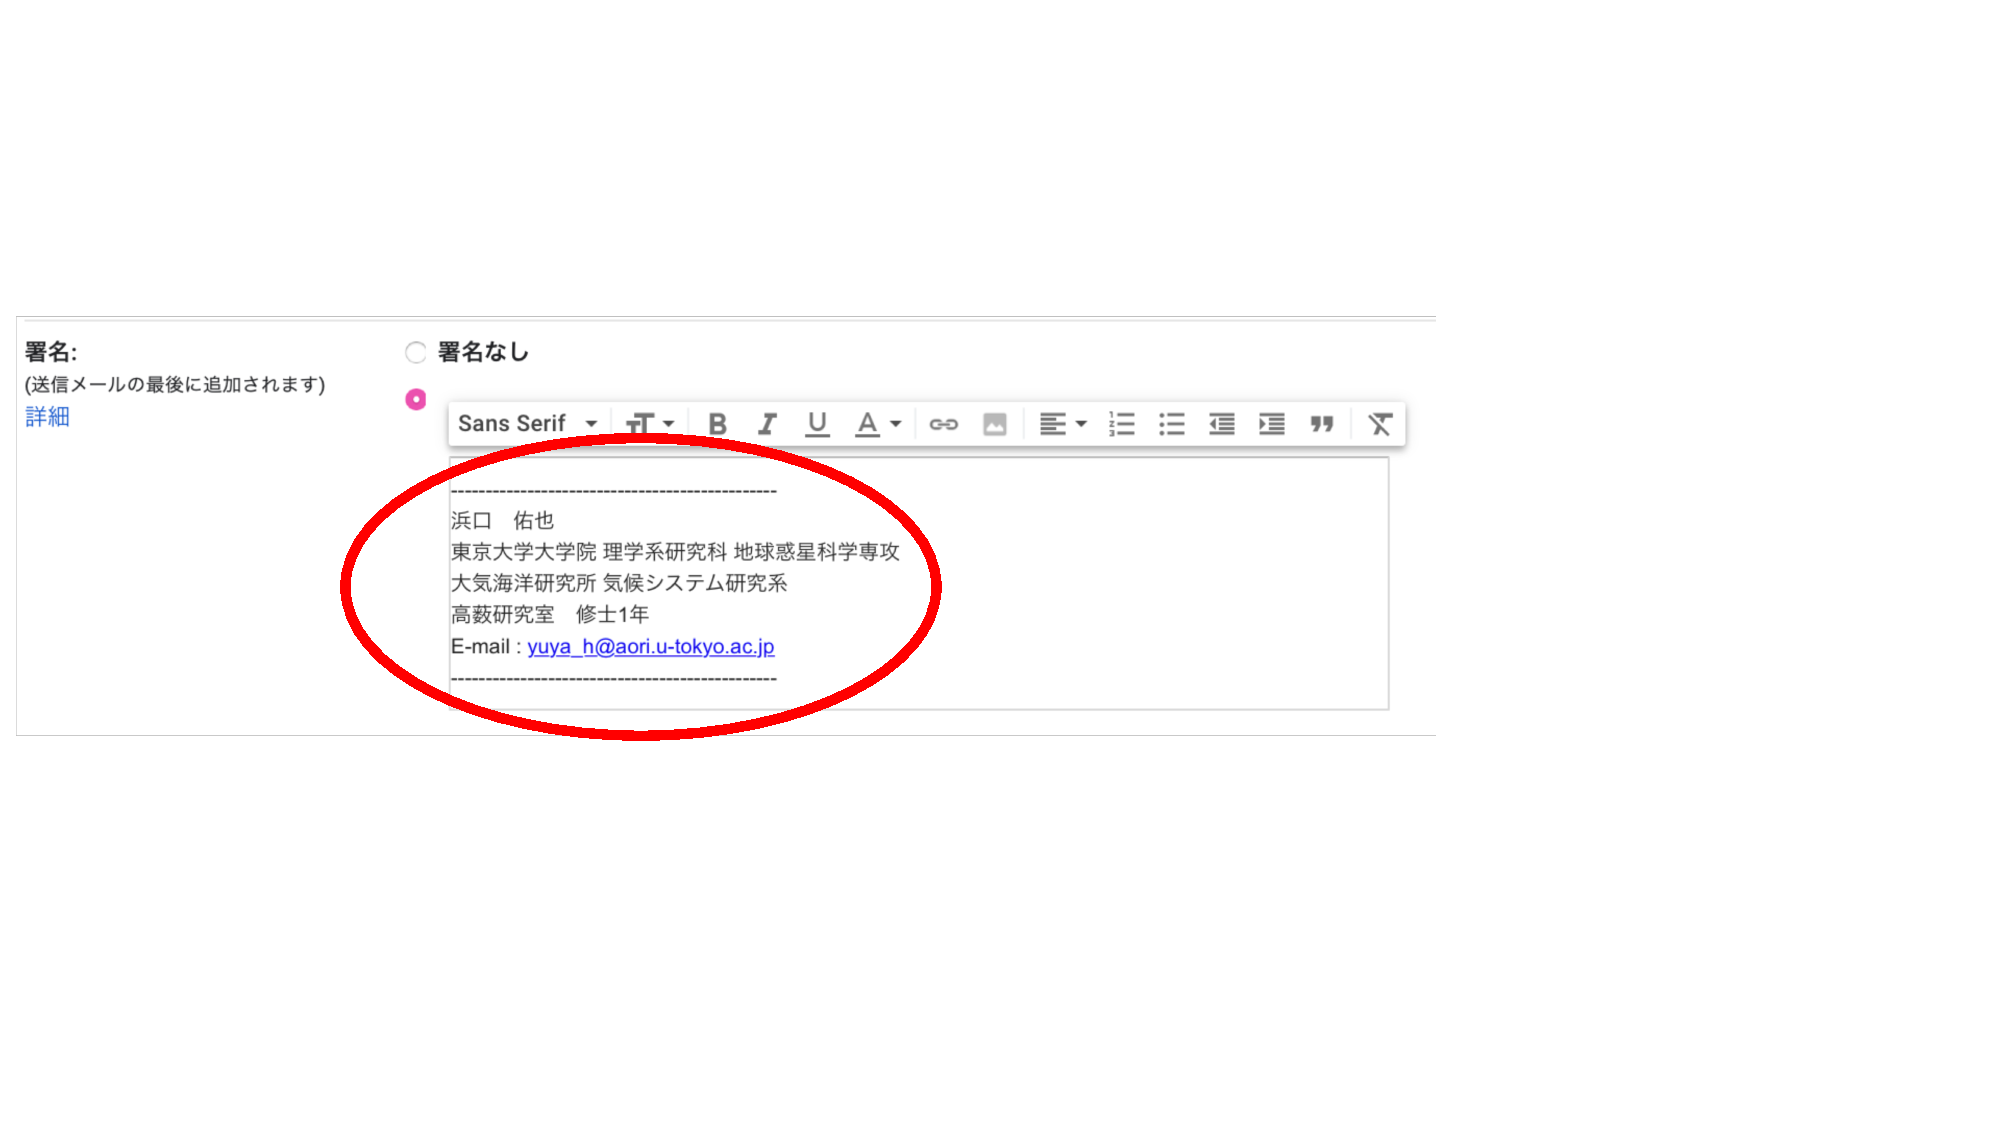
\includegraphics[width=140mm,pagebox=cropbox,clip]{fig/shomei.pdf}
\end{center}

\subsection{Thunderbird}
  Thunderbirdはmozillaプロジェクトによって提供されているフリーの{\bf メーリング
  ソフト}です.拡張性に富み,直感的な操作が出来るほか,いくつかのOS上
  (Windows, Mac, Linux)で同じように使えるのが特徴です.
  
  % \subsection{使ってみよう}
  % ではさっそくThunderbirdを起動してみましょう.先ほどと同様にターミナルを
  % 開き,\\
  % \quad \quad \quad {\bf{\$ thunderbird \&}}\\
  % と入力してください.次のようなウインドウが開き,Thunderbirdが起動しま
  % す.


%   次ページの表はそのときに必要なサーバー情報です.

% \begin{table}[ht]
%   \begin{center}
%   \begin{tabular}{|c|c|}\hline
% 受信サーバー & g.ecc.u-tokyo.ac.jp \\
% \hline
% 送信サーバー & g.ecc.u-tokyo.ac.jp \\
% \hline
% メールアドレス & $\langle$ 任意 $\rangle$ @g.ecc.u-tokyo.ac.jp \\
% \hline
% アカウント & $\langle$ 任意 $\rangle$ \\
% \hline
% パスワード & 各自のパスワード \\
%   \hline
%   \end{tabular}
%   \end{center}
%   \label{table2}
% \end{table}

% まずは,「{\bf 氏名またはニックネーム}」に適当な名前を入力し,
% 「{\bf メールアカウントを設定する}」をクリックします.
% すると,以下のような画面が現れますので,
% 「{\bf あなたの名前}」,「{\bf メールアドレス}」,「{\bf パスワード}」を入力してください
% (下の画面はこれらを入力したところ).
% 入力したら,「{\bf 続ける}」をクリックします.

% \begin{center}
% \includegraphics[width=75mm,pagebox=cropbox,clip]{bird1_2015.pdf}
% \end{center}

% 画面が広がりますから,受信サーバと送信サーバのホスト名に適切なものを
% 入力してください(受信サーバ,送信サーバともに\ .g.ecc.u-tokyo.ac.jpと
% なっていると思うので,最初の「{\bf .}」を消して下さい).

% なお「{\bf Thunderbirdはあなたのアカウント設定を見つけられませんでした.}」
% のメッセージはとりあえず無視しておいて大丈夫です.

% 次に,受信サーバの「{\bf ポート番号}」として「{\bf 993}」,
% 送信サーバの「{\bf ポート番号}」として「{\bf 465}」を選択します(選択に伴い,「SSL」や「認証方式」は自動で変わるので特に変更する必要はありません).

% 入力が終ったら「{\bf 再テスト}」をクリックしてください.
% 「{\bf 次のアカウント設定が,指定されたサーバを調べることにより見つかりました.}」
% というメッセージが表示されます.
% 後は,「{\bf 完了}」をクリックすれば設定は完了です.

% \begin{center}
% \includegraphics[width=120mm,pagebox=cropbox,clip]{bird2_2015.pdf}
% \end{center}

%Thunderbirdは直感的に操作が行いやすいので,上でやった以上
%の実用指南は特に載せません.また,同ソフトの特徴である拡張機能につい
%ては興味のある人は以下のURLを参照したりgoogle先生に聞いてみるなどして調
%べてみてください.\href{http://mozilla.jp/thunderbird/}{http://mozilla.jp/thunderbird/}

\subsubsection{メールアカウント設定}
eduにインストールされたThunderbirdにECCSクラウドメールを設定する方法を説明します.
自分のWindows PCやMacでも同様にして設定できるはずです.

LaunchpadからThunderbirdを起動します.
次のようなウインドウが開きます.\
\begin{figure}[H]
  \centering
  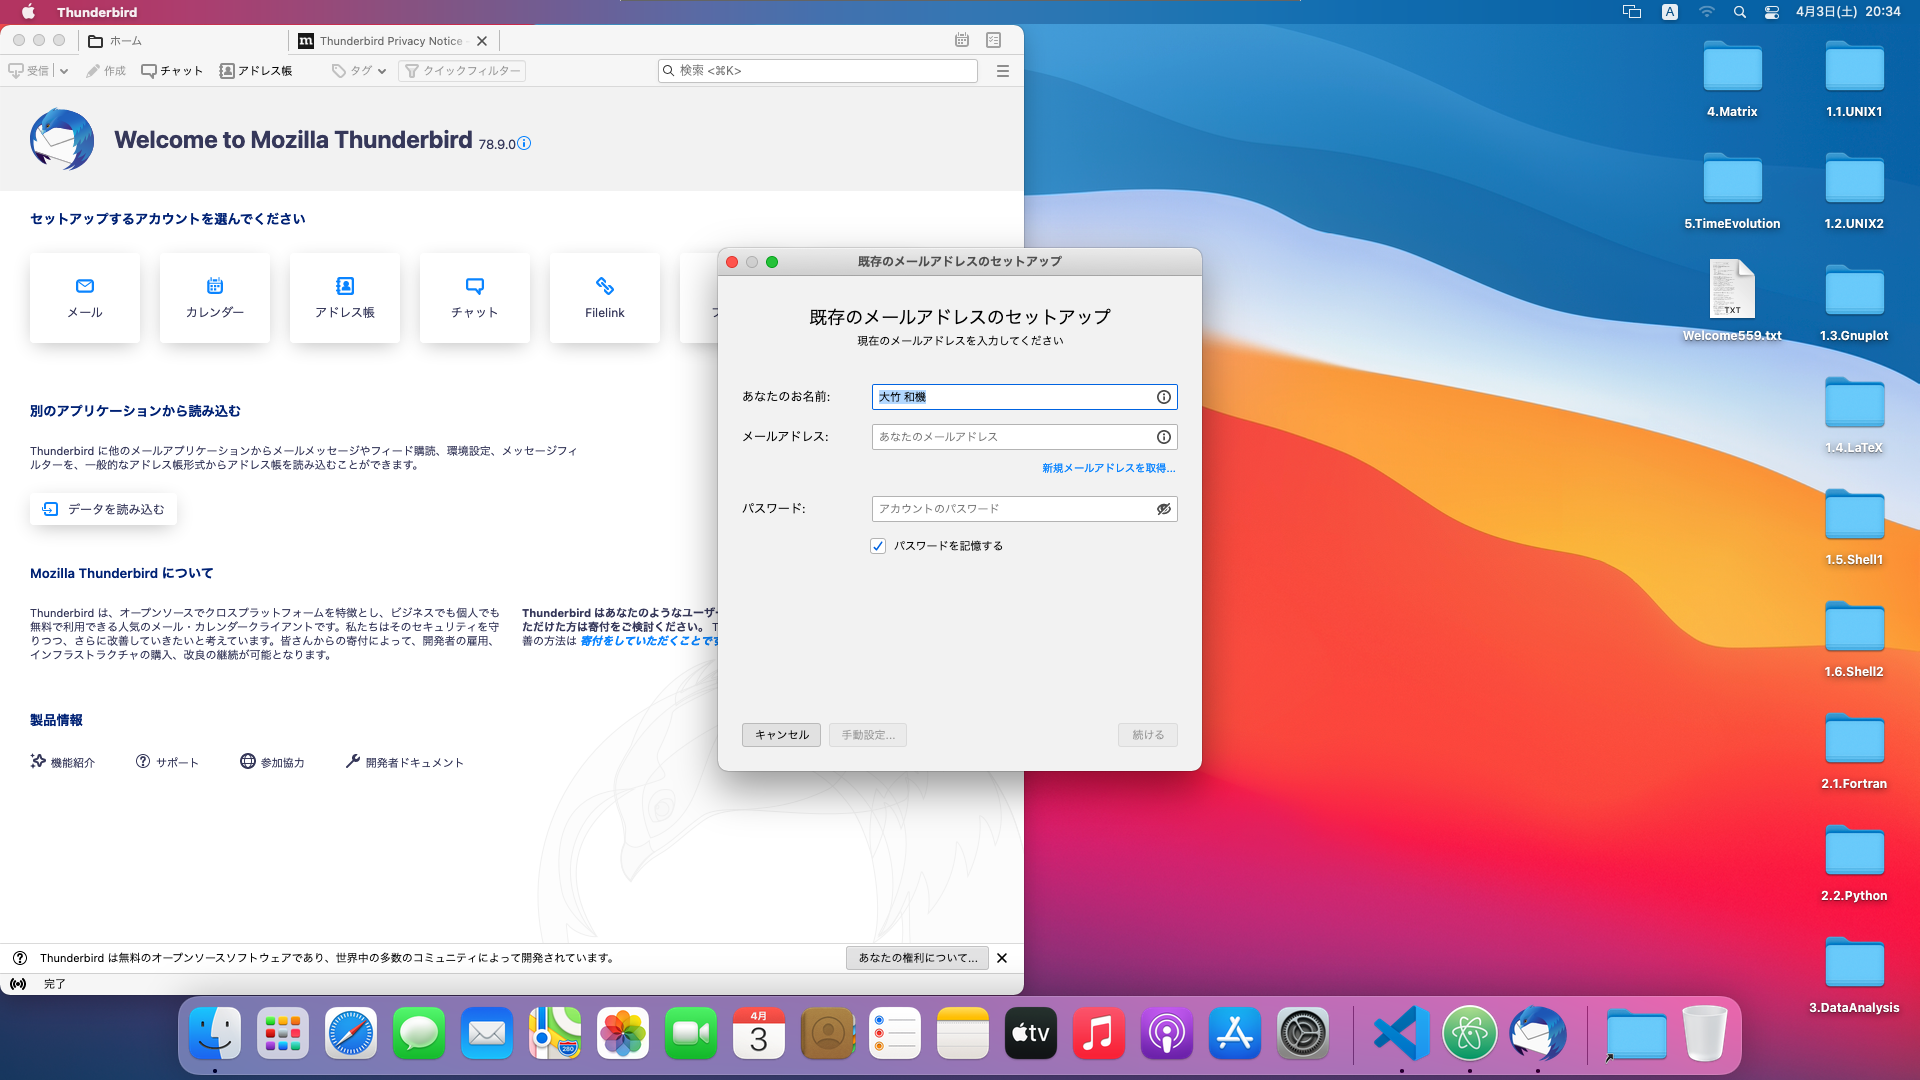
\includegraphics[height=7.5cm]{fig/MacThunderbird1.png}
\end{figure}
ECCSクラウドメールのアドレスを入力し,パスワードは空欄のまま,「続ける」をクリックします.

\newpage
すると「アカウント設定がMozilla ISP データベースから見つかりました.」と表示されます.
もし表示されなければ,メールアドレスが間違っています.
プロトコルが「IMAP(リモートフォルダー)」になっていることを確認し,「完了」をクリックします.
\begin{figure}[H]
  \centering
  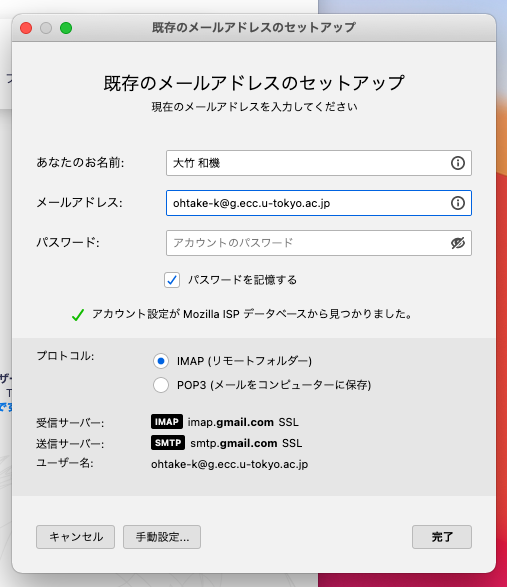
\includegraphics[height=10cm]{fig/MacThunderbird2trim.png}
\end{figure}

するとGoogleのログイン画面が表示されるので,「次へ」をクリックします.
\begin{figure}[H]
  \centering
  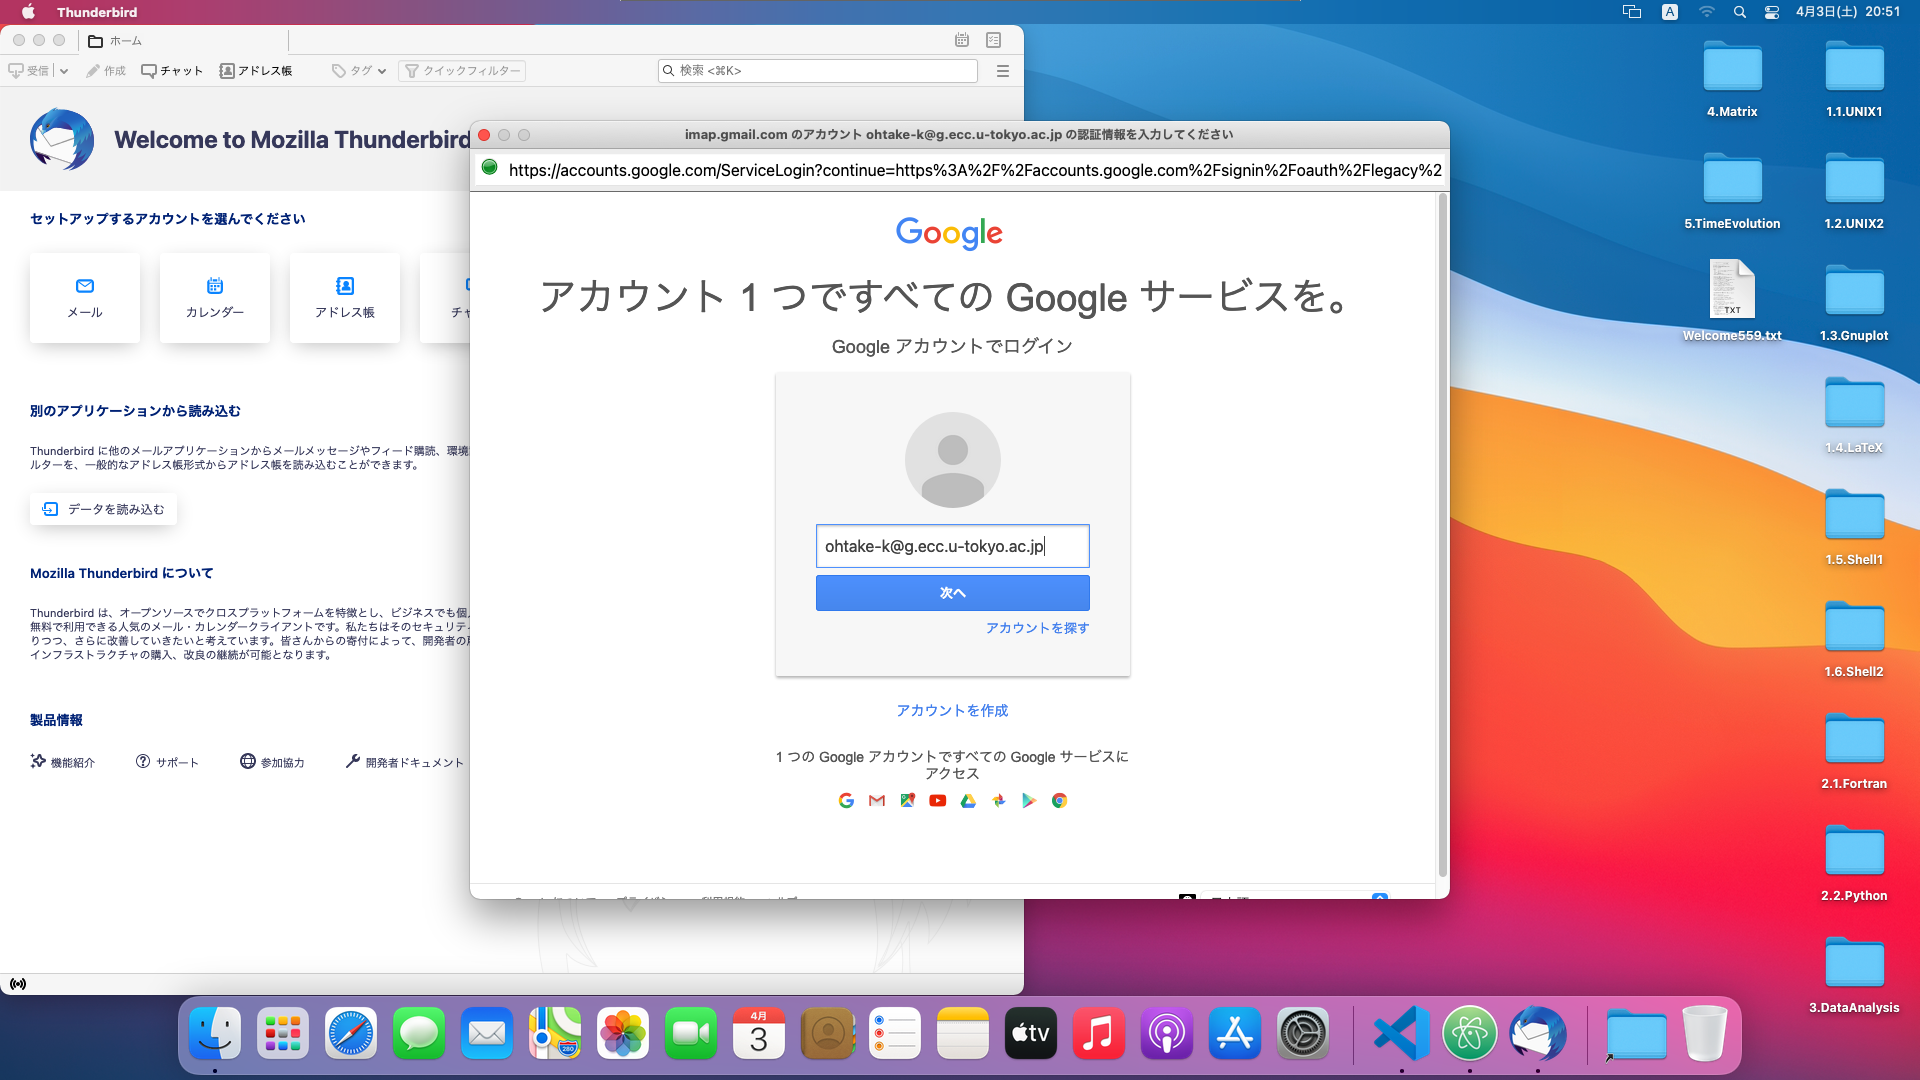
\includegraphics[height=7.5cm]{fig/MacThunderbird3.png}
\end{figure}

ECCSクラウドメールのパスワードを入力し,本人確認が表示されたら指示に従います.

\newpage
「許可」をクリックします.
\begin{figure}[H]
  \centering
  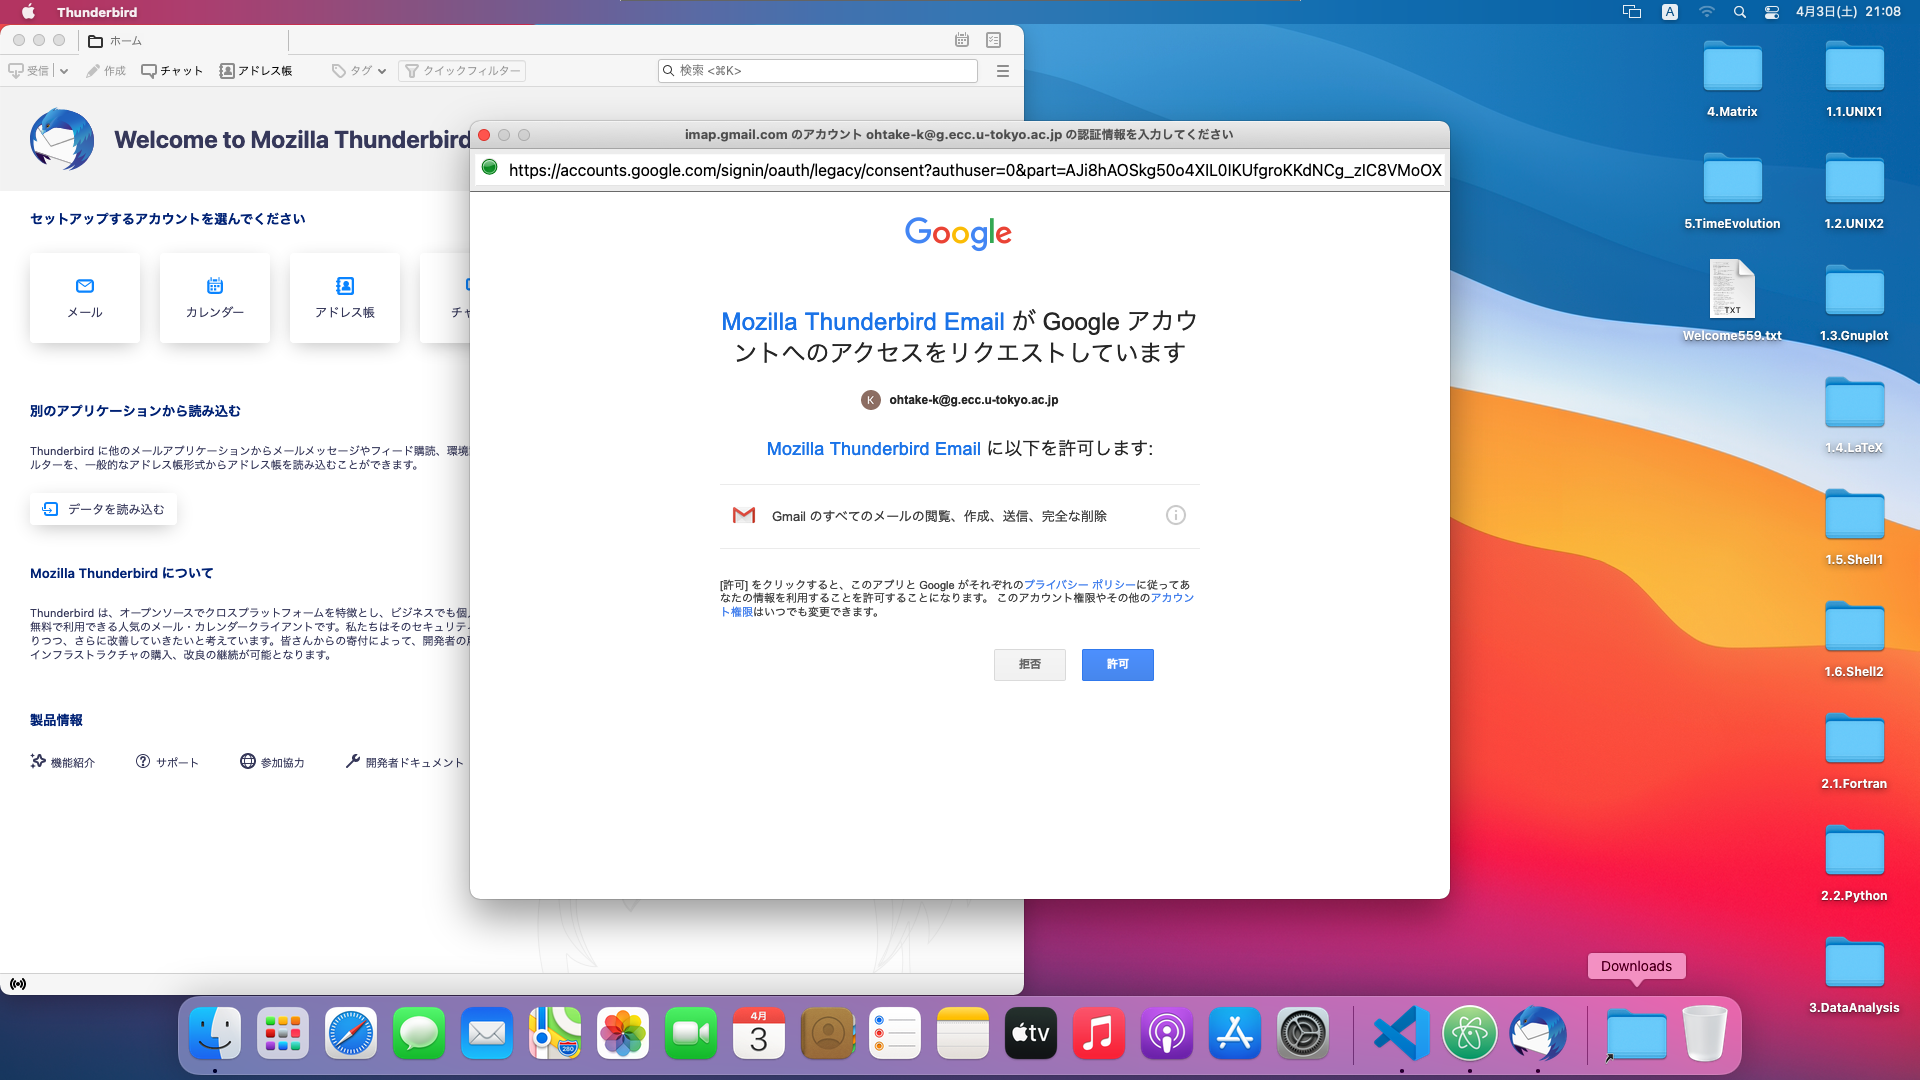
\includegraphics[height=7.5cm]{fig/MacThunderbird4.png}
\end{figure}

「デフォルトとして設定」をクリックします.
\begin{figure}[H]
  \centering
  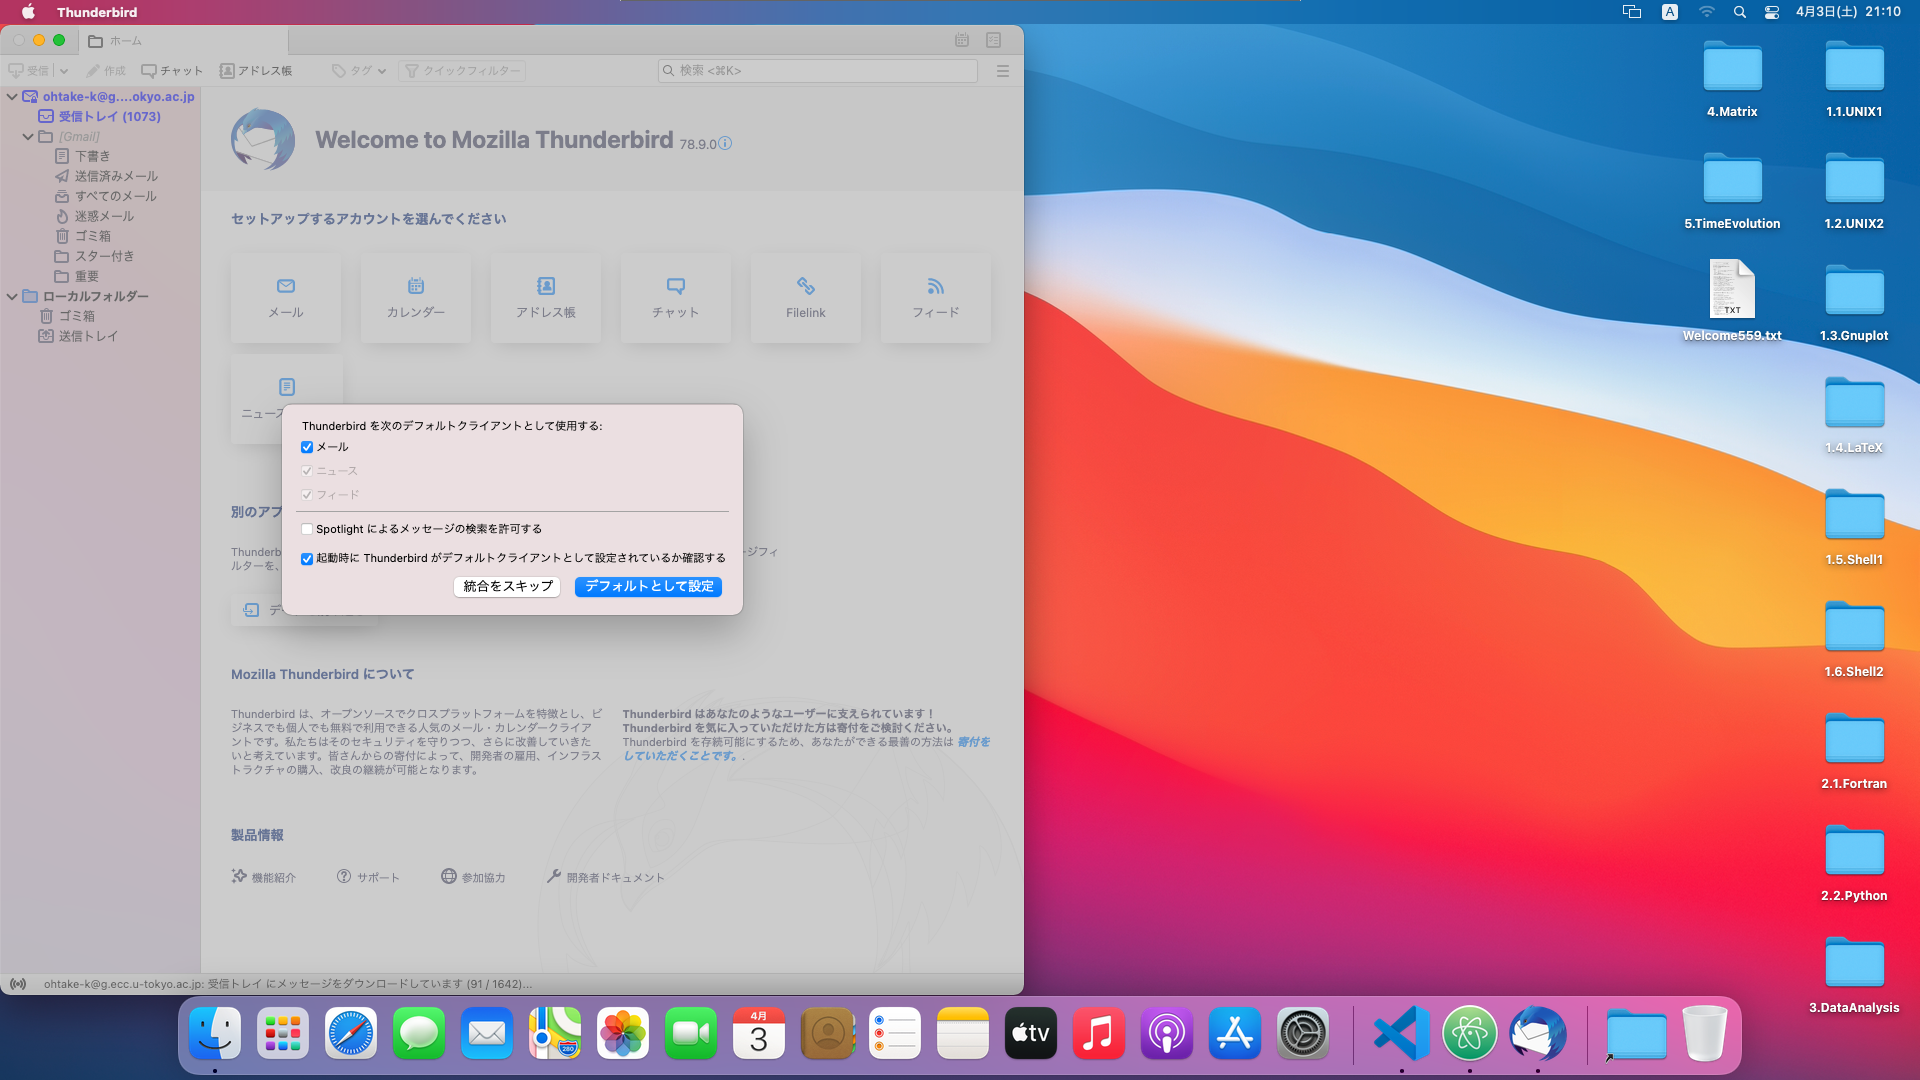
\includegraphics[height=7.5cm]{fig/MacThunderbird5.png}
\end{figure}

\newpage
メールが表示されたら,設定完了です.
\begin{figure}[H]
  \centering
  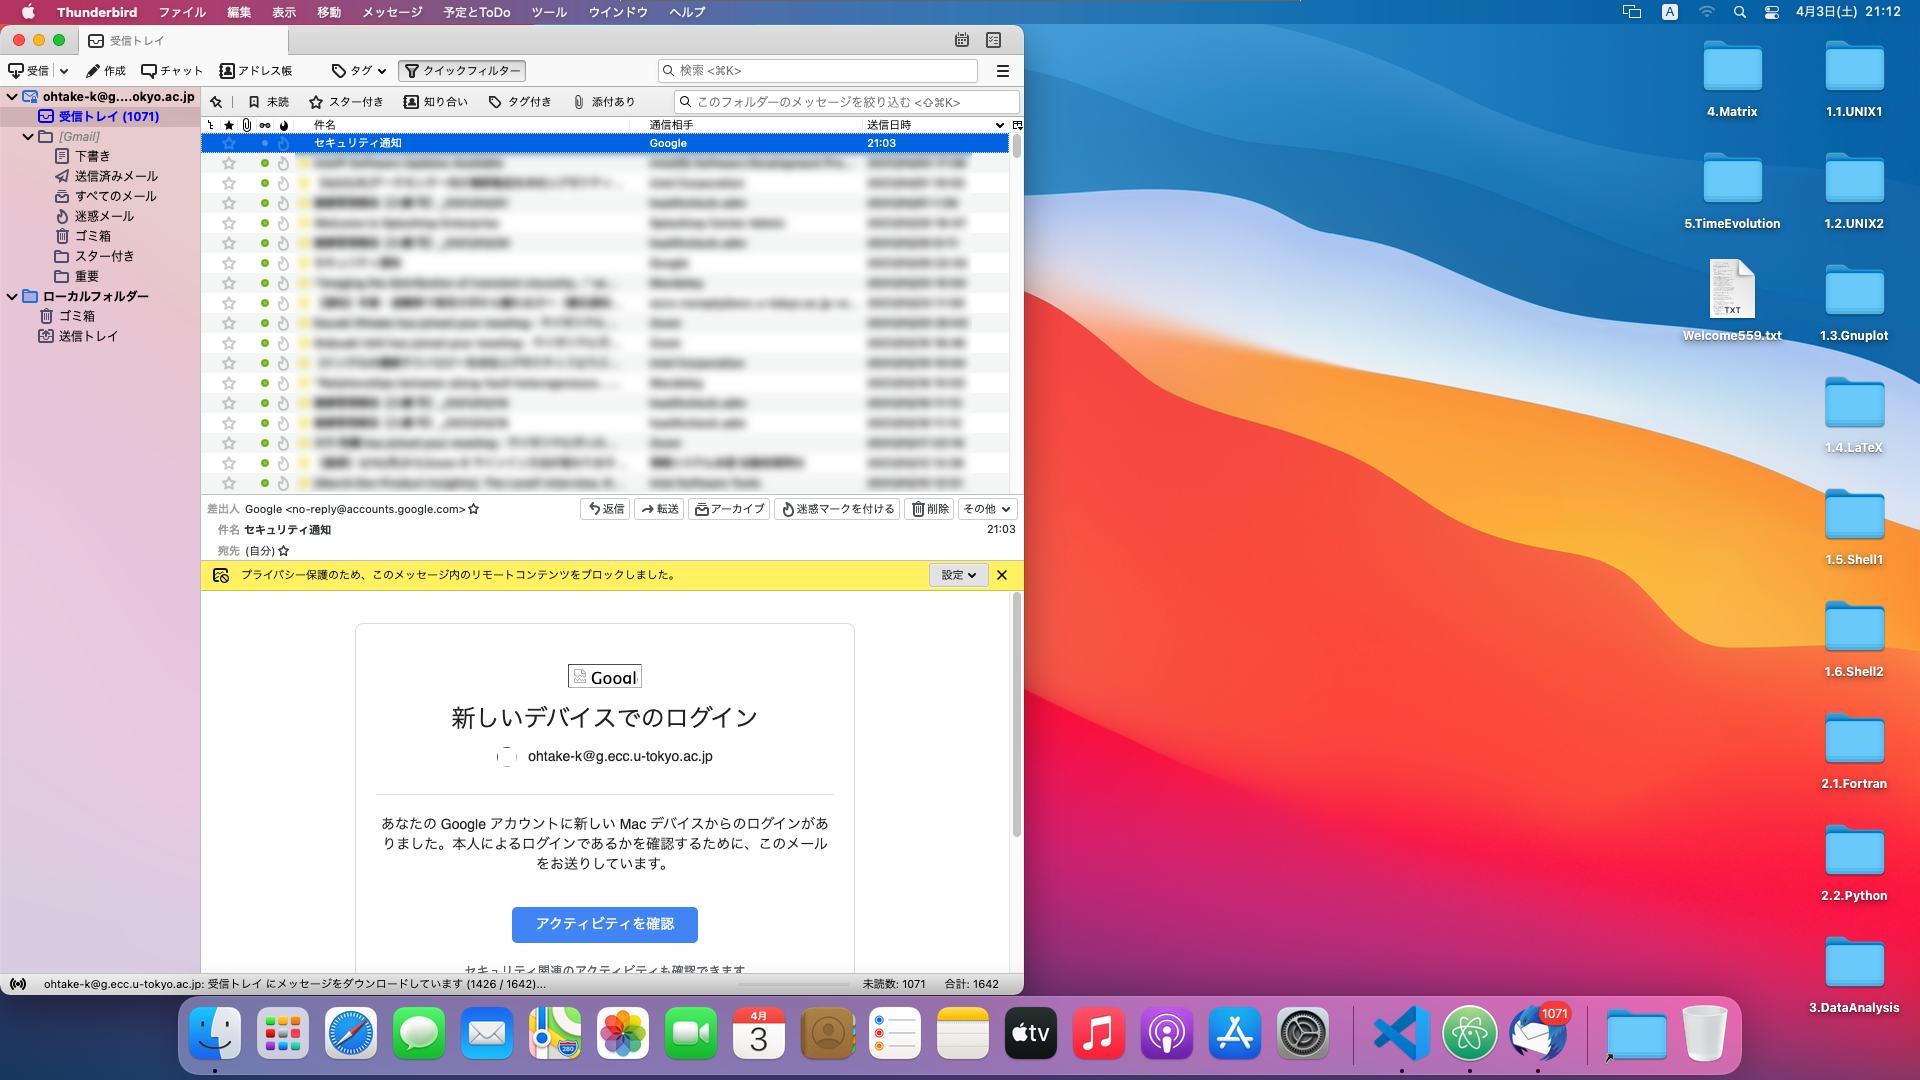
\includegraphics[height=7.5cm]{fig/MacThunderbird6.png}
\end{figure}

\subsubsection{署名の作成}
「ツール」→「アカウント設定」とクリックします.
\begin{figure}[H]
  \centering
  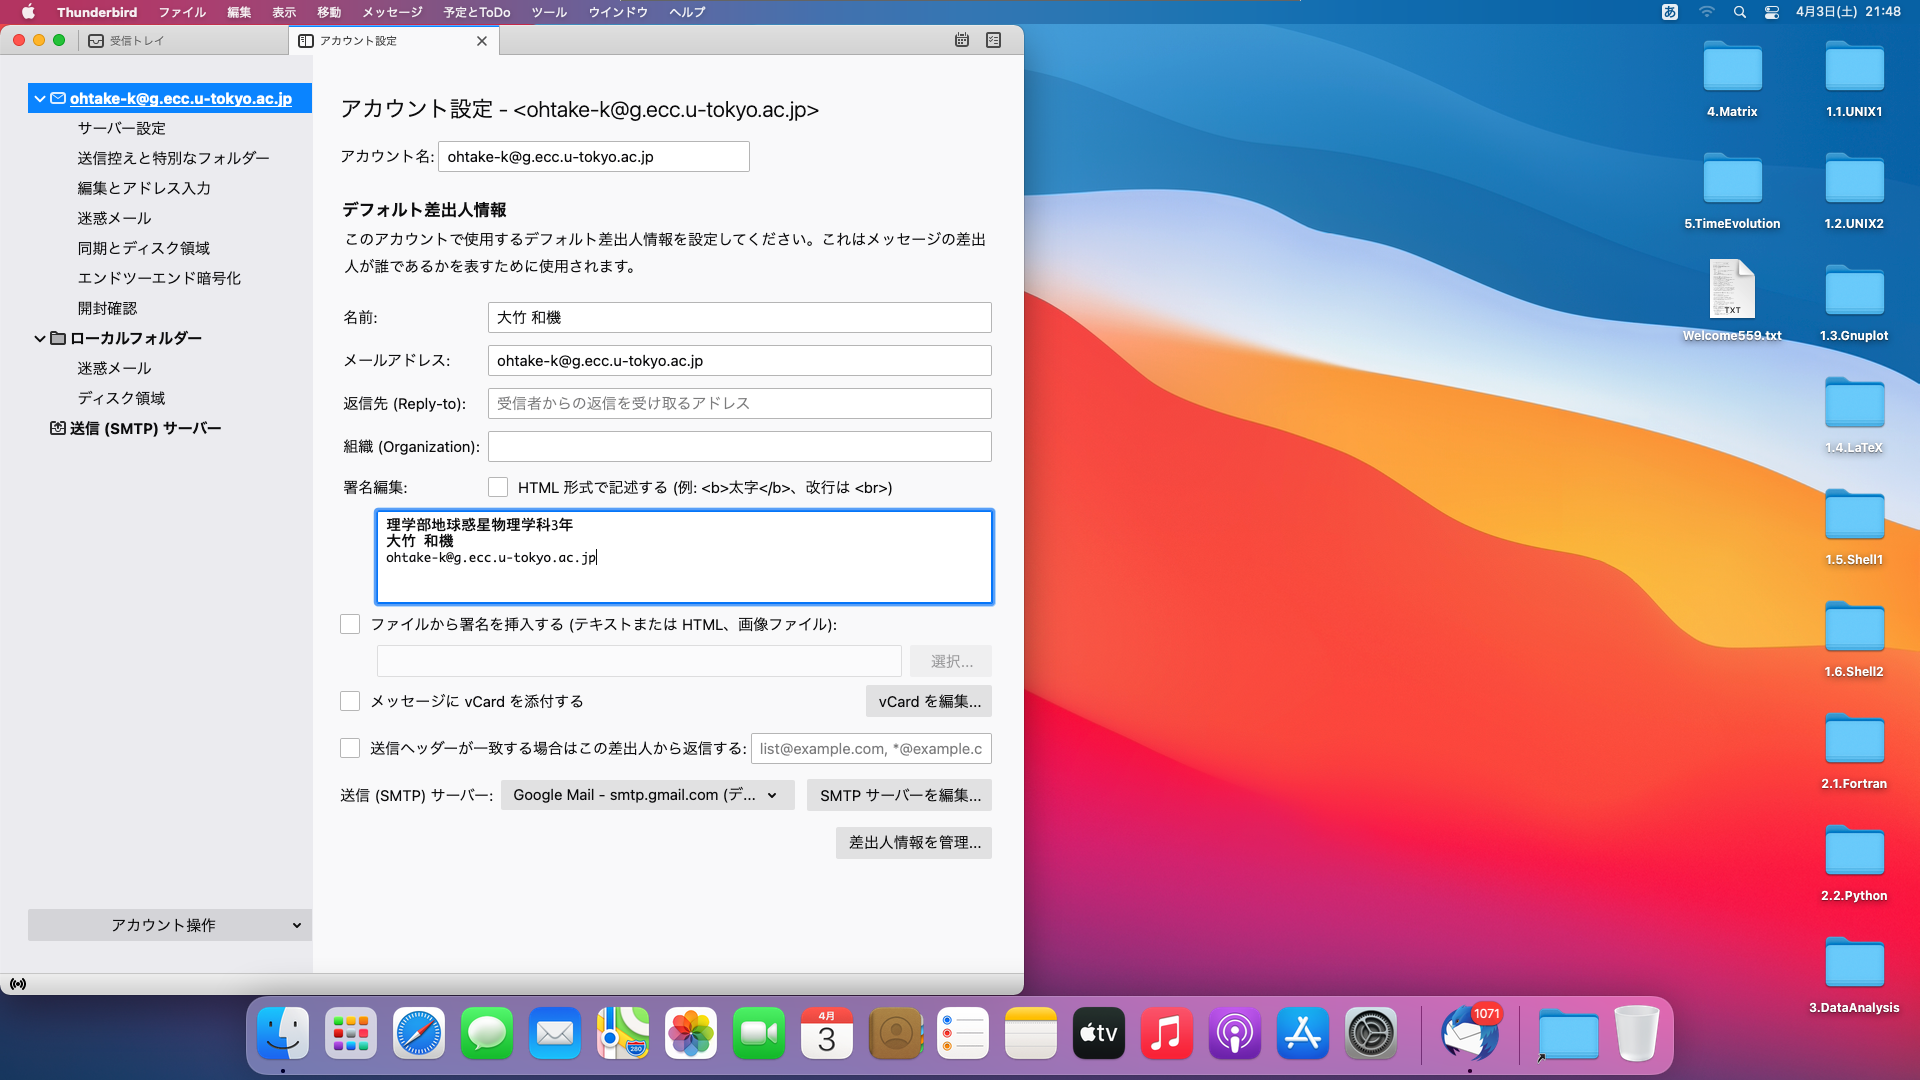
\includegraphics[height=7.5cm]{fig/MacThunderbird7.png}
\end{figure}
「署名編集」の欄に署名を作成します.

\subsection{Slack}
Slackとは、ビジネス用チャットアプリです。
計算機演習では、授業に関する連絡手段や質問の場としてSlackを使います。
こまめにチェックできるように、自分のパソコンにSlackアプリをインストールしましょう。
また自宅にいて自分で調べてもわからないことは、Slackで遠慮なく教員やTAに質問してください!

\newpage
\section{テキストエディタ}
テキストエディタとは,文字や記号などのテキストで構成されているテキストファイルを編集するソフトのことです.Windowsのメモ帳などもテキストエディタの一つです.本章ではメジャーな3つのテキストエディタについて紹介します.使用するエディタはどれでも構わないですが,最低どれか一つを使ってファイルの編集をできるようになりましょう.
\subsection{Emacs}
Emacsはテキストエディタの一つです.ターミナル上でファイルの確認や編集を行うことができます.また,ファイルの編集以外にもEmailの送受信をしたり,簡単なゲーム(テトリスなど)をしたりすることもできます.ここでは基本的な機能であるファイル編集について見ていきましょう.
% \subsection{Emacsとは}
% % では,より実践的な内容として今後プログラミングをしていく上で頻繁に使うことになる{\bf Emacs}について勉強しましょう.

% Emacsは{\bf テキストエディタ}です(簡単に言えばメモ帳の上位互換).主にファイルの編集を行いますが,他にもEmailの送受信,プログラムのコンパイル,シェルによる対話作業などを扱うこともで
% きます(コンパイルやシェルなどの意味は現時点でわからなくても問題ありません).
% 今回はファイル編集の練習を中心に,まずはEmacsに慣れてもらいます.

% \begin{flushright}
% "Emacs is the extensible, customizable, self-documenting realtime display editor"\\
% \end{flushright}

% \subsection{使ってみよう}
% \subsubsection{起動}
% まずはさっそくEmacsを起動しましょう.ターミナル上でのコマンド入力によって起動します.\\
% \quad \quad \quad {\bf{emacs \&}}\\
% と入力してください.下のようなウインドウが開き,Emacsが起動します.

% \begin{figure}[ht]
%   \begin{center}
%     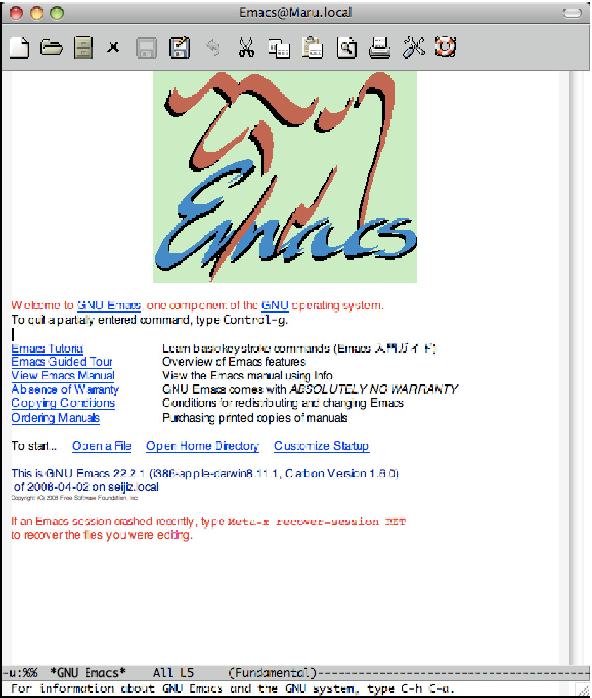
\includegraphics[width=70mm,pagebox=cropbox,clip]{fig/emacs001.pdf}
%   \end{center}
% \end{figure} 

% まず目につくのは上部の広いワークスペースです.ファイルの編集はこの部分
% で行います.次に下の方を見てください.下から2行目にEmacsの動作状況につ
% いてたくさん表示されています.この行を{\bf モードライン}と呼びます.モードライ
% ンの下の部分は{\bf ミニバッファ}と呼ばれます.ミニバッファは入力中のコマンドを
% Emacsが表示するための領域として,またファイルを読み込むときにファイル名
% を指定するための領域として,あるいはまたサーチや置換の対象となる文字列を
% 入力する時の領域として利用されます.

\subsubsection{ファイルを開く}
まずはさっそくEmacsを起動してファイルを表示しましょう.ターミナル上で以下のコマンドを入力してください.\\
\quad \quad \quad {\bf{emacs -nw ./text.txt}}\\
するとあなたがいるディレクトリに\verb| text.txt |というファイルが作られ,同時にEmacsの編集画面が立ち上がります. \ \footnote{ディレクトリについては次回の授業で学びます.}

なお,ファイル名のところ(上の例では./text.txt)は,既に存在するファイルを指定すればそのファイルが開かれます.ファイルが存在しない場合に,新しいファイルが作られます.

\subsubsection{ファイルの保存}
ファイルをそのままの名前で保存したい場合には,CTRL-x CTRL-sと入力してく
ださい.また別名で保存したい場合にはCTRL-x CTRL-wと入力し,ミニバッファ
にファイル名を入力してEnterを押してください.ただし,-(ハイフン)は「同時押し」の意味です.(これ以降も「同時押し」の意味で-表記します.)

\subsubsection{終了}
Emacsを終了する時はCTRL-x CTRL-cと入力してください.

\subsubsection{作業中止}
現在行っている作業を中止したいときにはCTRL-gと入力します.

% \subsection{ファイル編集}
% \subsubsection{ファイルを開く}
% 次はEmacsを使ってファイルの編集を行ってみましょう.ファイルを開くために
% はCTRL-x CTRL-fと入力します.すると,ミニバッファに

% \begin{figure}[ht]
%   \begin{center}
%     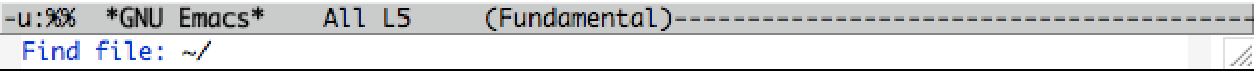
\includegraphics[width=130mm,pagebox=cropbox,clip]{fig/emacs002.pdf}
%   \end{center}
% \end{figure}

% \noindent
% と表示されます.ここにファイル名を入力してEnterを押してください(例えば $\sim$/test.txt).なお,
% 入力したファイルが存在しない場合はその名前の新規ファイルが作成されます.

% \subsubsection{新しくウィンドウを開かないでファイルを開く}
% ターミナル上で以下のコマンドを入力すると,直接ファイルを開いて編集することができます.\\
% \quad \quad \quad {\bf{emacs -nw 開きたいファイル名}}\\
% 開きたいファイル名は例えば$\sim$/test.txtのようなものです.入力したファイルが存在しない場合はその名前の新規ファイルが作成されます.

% \subsubsection{日本語入力}
% 日本語入力に切り替えるためには CTRL-$\backslash$ (バックスラッシュ)と入力します.日本語変換の際に便利なコマンドの一覧は次節にまとめてあります.

% \subsection{便利な機能} 
\subsubsection{コピー\&ペースト or カット\&ペースト}
文章を編集している際に,よく使うテクニックにコピー\&ペーストとカット\&
ペーストというものがあります.前者は選択した部分を残して,その複写を目的
の場所に貼付けることで,後者は選択した部分を削除し,その複写を目的の場所
に貼付けることを指します.Emacs上ではこれらの操作もコマンドで行います.

実際には次のように行います.
まずコピーしたい領域の最初の文字にカーソルを移動し,
CTRL-SPCまたはCTRL-@を押します.
すると,ミニバッファに

\begin{figure}[ht]
  \begin{center}
    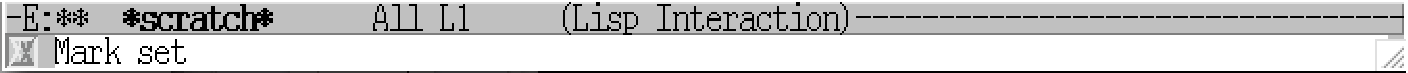
\includegraphics[width=130mm,pagebox=cropbox,clip]{fig/emacs003.pdf}
  \end{center}
\end{figure}

\noindent
と表示されます.次に,コピーしたい領域の最後の文字までポイントを移動させ
ます.移動が完了したら{\bf ESC-w}でコピー,{\bf CTRL-w}でカットします.最後に目的の
場所で{\bf CTRL-y}を押せばペーストできます.

あるいは行ごとカット\&ペースト(CTRL-k CTRL-y)を行うことでカットした行を復元しつつ,目的の場所で{\bf CTRL-y}を押すことで行を簡単に複製できます.今後プログラムを書く作業で重宝するので心に留めておきましょう.

\subsubsection{操作の取り消し}
一つ前の操作を取り消したい時はCTRL-/ と入力します.入力した回数だけ以前
の操作を取り消すことができます.

\subsubsection{その他のコマンド}
この他にも,{\bf 問い合わせ置換(ESC-\% [変換前の文字列] [変換後の文字列])}やシェルの起動,
コンパイルなど多くのコマンドがあります.適宜調べて使ってみて下さい.
作業がずっとスムーズにできるようになると思います.

\subsubsection{便利なショートカットコマンド一覧}

\begin{table}[H]
 \begin{minipage}{0.5\hsize}
  \begin{center}
    \begin{tabular}{|c|c|c|}\hline
      使用時 & 操作  & コマンド \\
      \hline
      一般 & {\bf ファイル検索}& C-x C-f  \\
      & {\bf ファイル保存} & C-x C-s  \\
      & {\bf 別名で保存}  & C-x C-w \\
      & {\bf 終了}            & C-x C-c  \\
      ポインタの移動 & 前の行に移動    & C-p \\
      & 次の行に移動    & C-n \\
      & 右に移動          & C-f  \\
      & 左に移動          & C-b  \\
      & 行の最初に移動 & C-a  \\
      & 行の最後に移動 & C-e  \\
      & 次の頁に移動    & C-v  \\
      & 前の頁に移動    & Esc-v     \\
      & バッファの最初に移動 & C-x [ \\
                      & バッファの最後に移動 & C-x ] \\
   \hline
  \end{tabular}
  \end{center}
  \label{table:one}
 \end{minipage}
 \begin{minipage}{0.5\hsize}
  \begin{center}
  \begin{tabular}{|c|c|c|}\hline
    使用時 & 操作  & コマンド \\
  \hline
  削除  & 右の文字を削除 & C-d \\
  & 左の文字を削除 & C-h \\
        	& {\bf 行末まで削除} & C-k \\
          ペースト(貼り付け)   &  {\bf 削除したものをペースト} & C-y \\
日本語変換  & 右の文節に移る  & C-f  \\
                & 左の文節に移る  & C-b \\
                & 文節を伸ばす     & C-o  \\
                & 文節を短くする  & C-i \\
                &  変換を確定する  & RET \\
ウインドウ分割 & 上下に分割 & C-x 2\\
                      & 左右に分割 & C-x 3 \\
                      & 他を消去 & C-x 1  \\
                      & 現在のを消去 & C-x 0 \\
                      & 他に移動 & C-x o \\
                      \hline
                    \end{tabular}
                  \end{center}
                  \label{table:two}
                \end{minipage}
              \end{table}
              
※なお,上記の表では略記号を用いています.(例:C-x C-f → CTRL-x CTRL-f,
C-x 1 → CTRL-x 1など)

※特に重要なものを太字で記載.


\subsubsection{参考になりそうなページ}
\noindent
GNU EmacsのHP(\url{https://www.gnu.org/software/emacs/emacs.html}) \\
慶應大学のページ(\url{https://cns-guide.sfc.keio.ac.jp/2000/4/index.html})\\
ショートカット一覧(\url{https://qiita.com/katsuta/items/7d492889820008d55e3b})

\subsection{vim}
Emacsと並んで広く使われているテキストエディタ「vim」について説明します.\

\subsubsection{vimとは}
vimはEmacsと人気を二分するテキストエディタです.ターミナル上で,{\bf キーボードのみを使って操作ができる}(マウスを使う必要がない)ことが大きな特徴です.このためSSH先のリモートマシン上のテキストを編集する用途で特に好まれます.以下ではvimのごく基礎的な操作方法を解説します.なお日本語入力の状態ではvimのコマンドを打つことができないため,あらかじめ英字モードに切り替えておいてください.\

\subsubsection{ファイルを開く}
ターミナル上で\ \\
\quad \quad \quad {\bf{vi ./text.txt}}\\
と入力してみましょう.するとあなたがいるディレクトリに\verb| text.txt |というファイルが作られ,同時にvimの編集画面が立ち上がります. \ \footnote{ディレクトリについては次回の授業で学びます.}

\subsubsection{文字を入力する}
vimは起動時点で,{\bf ノーマルモード} というモードになっています.ノーマルモードではカーソルの移動を行うことができますが,現段階でこのテキストファイルは空ですからカーソル移動の練習は不可能です.まずは何か文字を入力してみましょう.\\
 文字を入力するためには,{\bf 挿入モード}に切り替える必要があります.{\bf i}のキーを押すと,挿入モードに入ることができます.複数行にわたって適当な文字列を打ち込んでみてください.入力が終わったら、{\bf esc}キーを押してノーマルモードに戻ります.\

\subsubsection{カーソル移動}
ノーマルモードで、以下のキーを押すとカーソル移動ができます.通常のカーソルキーを使うこともできますが,vimのコマンドを使うとホームポジションを崩すことなく高速に作業することができます.\

\begin{table}[H]
  \centering
  \begin{tabular}{|l|l|l|l|} \hline
    コマンド & 移動先 \\ \hline
    j & 一文字左 \\ \hline
    k & 一文字右 \\ \hline
    i & 一行上 \\ \hline
    m & 一行下 \\ \hline
    w & 次の単語の頭 \\ \hline
    e & 次の単語の末尾 \\ \hline
    0 & 行頭 \\ \hline
    \$ & 行末 \\ \hline
    gg & 最初の行 \\ \hline
    G & 最後の行 \\ \hline
  \end{tabular}
\end{table}

\subsubsection{文字を消す}
{\bf x}キーで一文字ずつ文字を消去できます. また{\bf dd}で一行まるごと消去できます.\

\subsubsection{元に戻す・やり直す}
{\bf u}キーで直前の操作を元に戻すことができます.また{\bf Ctrl+r}でやり直すことができます.\

\subsubsection{vimを閉じる}
テキストの編集が終わったら,{\bf :wq}と打ち込みましょう.作業内容を保存してvimを閉じることができます.{\bf :w}だけを打つと,ファイルの保存だけが行われます.作業内容を破棄してvimを閉じたいときは{\bf :q!}です.\

\subsubsection{チュートリアルで覚えよう!}
以上が、vimを使ってテキストを編集するために必要な最低限のコマンドです.しかしこれだけでは,vimを滑らかに操作して効率よく作業を進めることはできません.vimには,実際に練習しながら高度なコマンドを覚えられるチュートリアルが用意されています.ターミナルで\ \\
\quad \quad \quad {\bf{vimtutor}}\\
と打つとチュートリアルが始まります.ぜひ時間のあるときに,何度か繰り返し練習してみてください.\

\subsubsection{参考になりそうなページ}
\noindent
vim入門(\url{https://qiita.com/okamos/items/c97970ab34ff55ff3167})\\
vimコミュニティサイト(\url{https://vim-jp.org/})

\subsection{VSCode}
GUIベースで使用するテキストエディタとして,Visual Studio Code(VSCode)を紹介します.複数のファイルの編集からリモート接続まで様々なことをでき,非常に便利です.(ただし,edu端末でのVSCodeの使用にはかなり制限があるようです.edu端末での使用がうまくいかない場合は,自分のPCで試してみるかTAを呼ぶようにしてください.)

\subsubsection{起動}
LaunchpadからVisual Studio Codeを開きます.そうすると,以下のような画面が起動します.
\begin{figure}[H]
  \centering
  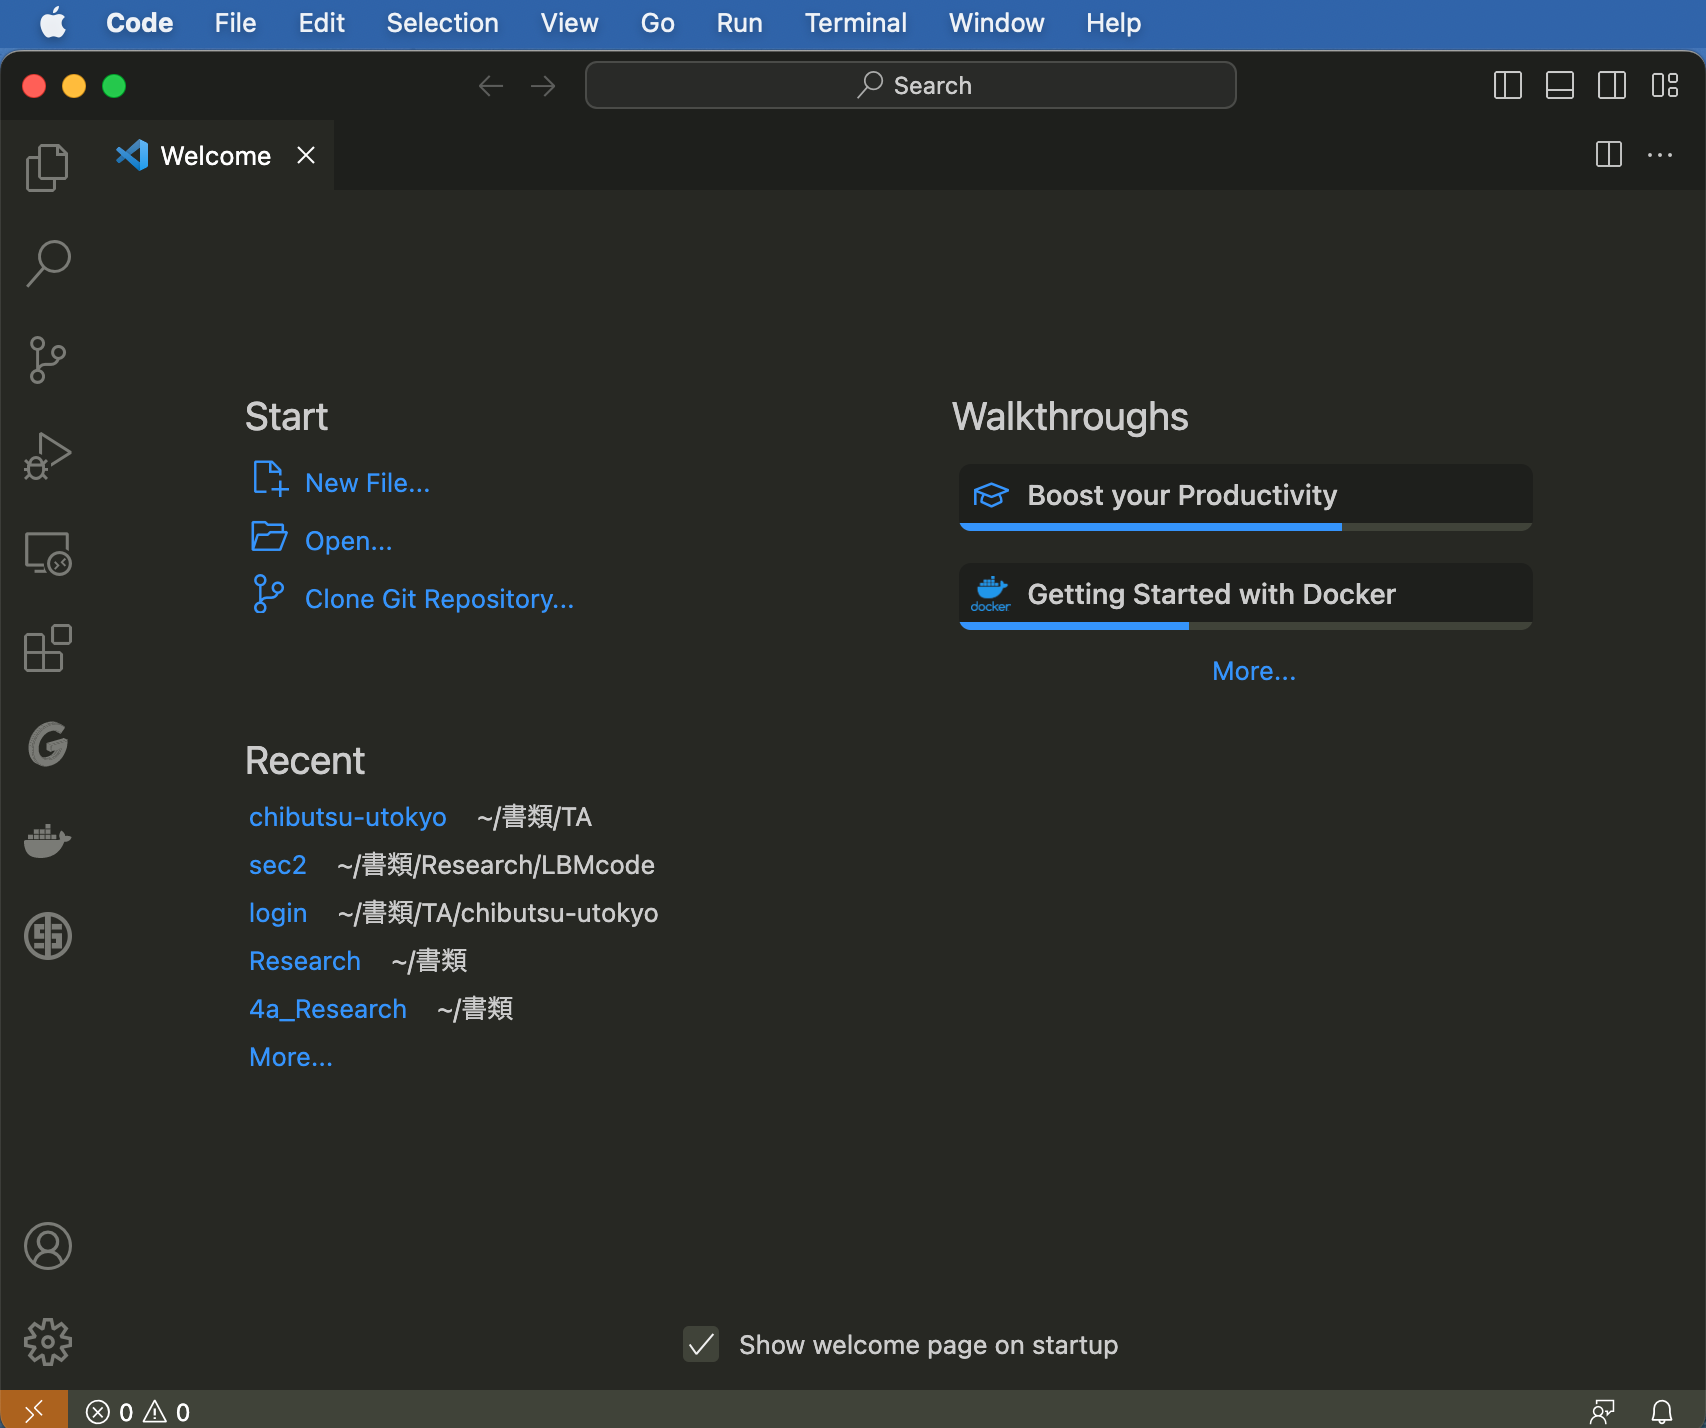
\includegraphics[height=7.5cm]{fig/VSCode1.png}
\end{figure}

\subsubsection{ターミナルからVSCodeを開く方法}
エディタで$\sim$/.bashrcファイルを開き編集します.適当な場所に以下の記述を追加して保存します.\\

追加する記述\\
\quad \quad \quad {\bf{export PATH=\$PATH:/Applications/Visual\textbackslash\ Studio\textbackslash\ Code.app/Contents/Resources/app/bin}}\\

例としてemacsでの編集の仕方を紹介します.まず,ファイルを開く\\
\quad \quad \quad {\bf{emacs -nw $\sim$/.bashrc}}\\

記述を追加

\begin{figure}[H]
  \centering
  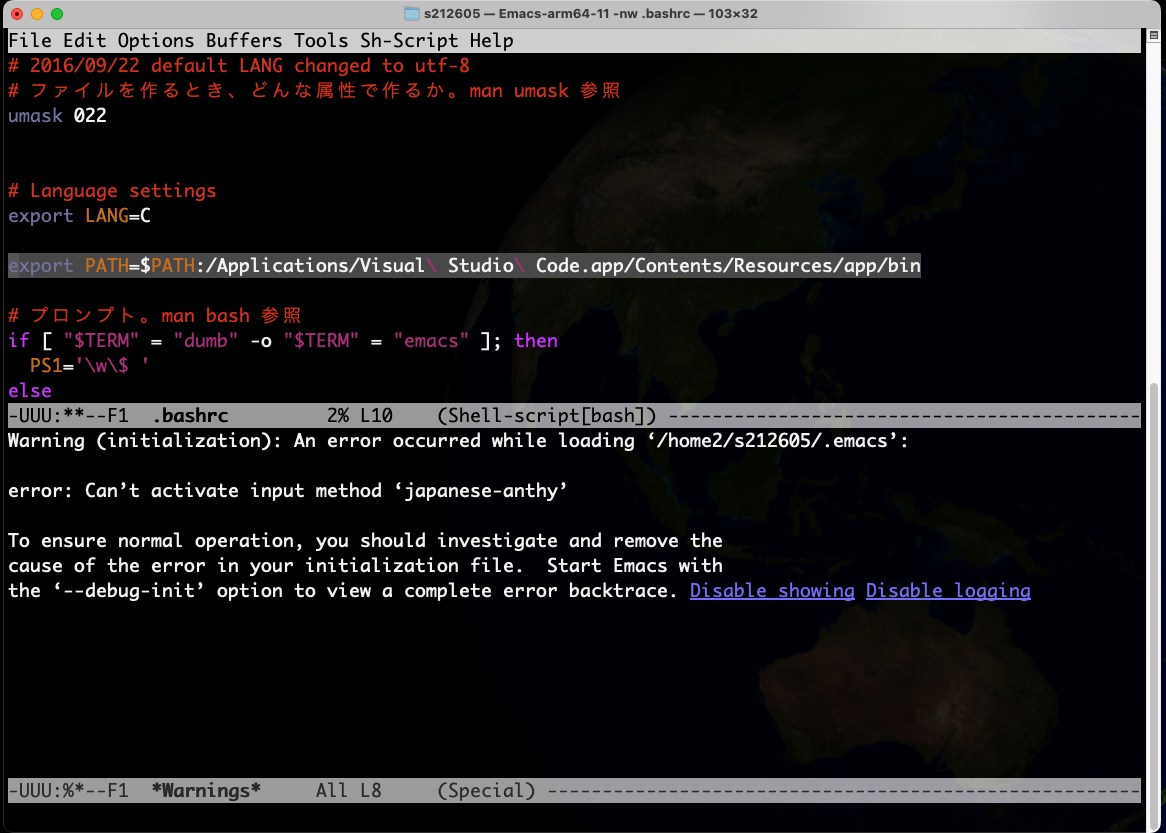
\includegraphics[height=7.5cm]{fig/VSCode5.png}
\end{figure}
CTRL-x\ CTRL-sでファイルを保存,CTRL-x\ CTRL-cでemacsを終了.\\

編集が終わったら,ターミナル上で以下のコマンドを実行してください.\\

\quad \quad \quad {\bf{source $\sim$/.bashrc}}\\

これで完了です.ターミナル上で{\bf{code}}と打ち込むとVSCodeが起動すると思います.\footnote{ここでやっているのはPATHを通すという作業です.詳しくはUNIXの第2回で習います.}

\subsubsection{日本語化}
デフォルトの言語は英語になっていますが,拡張機能をインストールすることにより日本語に変更することができます.Extensions(左端のバーの正方形が4つ並んでいるアイコン)をクリックし,検索窓にJapanese Languageと打ち込みます.Japanese Language Pack for Visual Studio Codeを選択して,installしましょう.(既にインストールされている場合はそのままで大丈夫です.)
\begin{figure}[H]
  \centering
  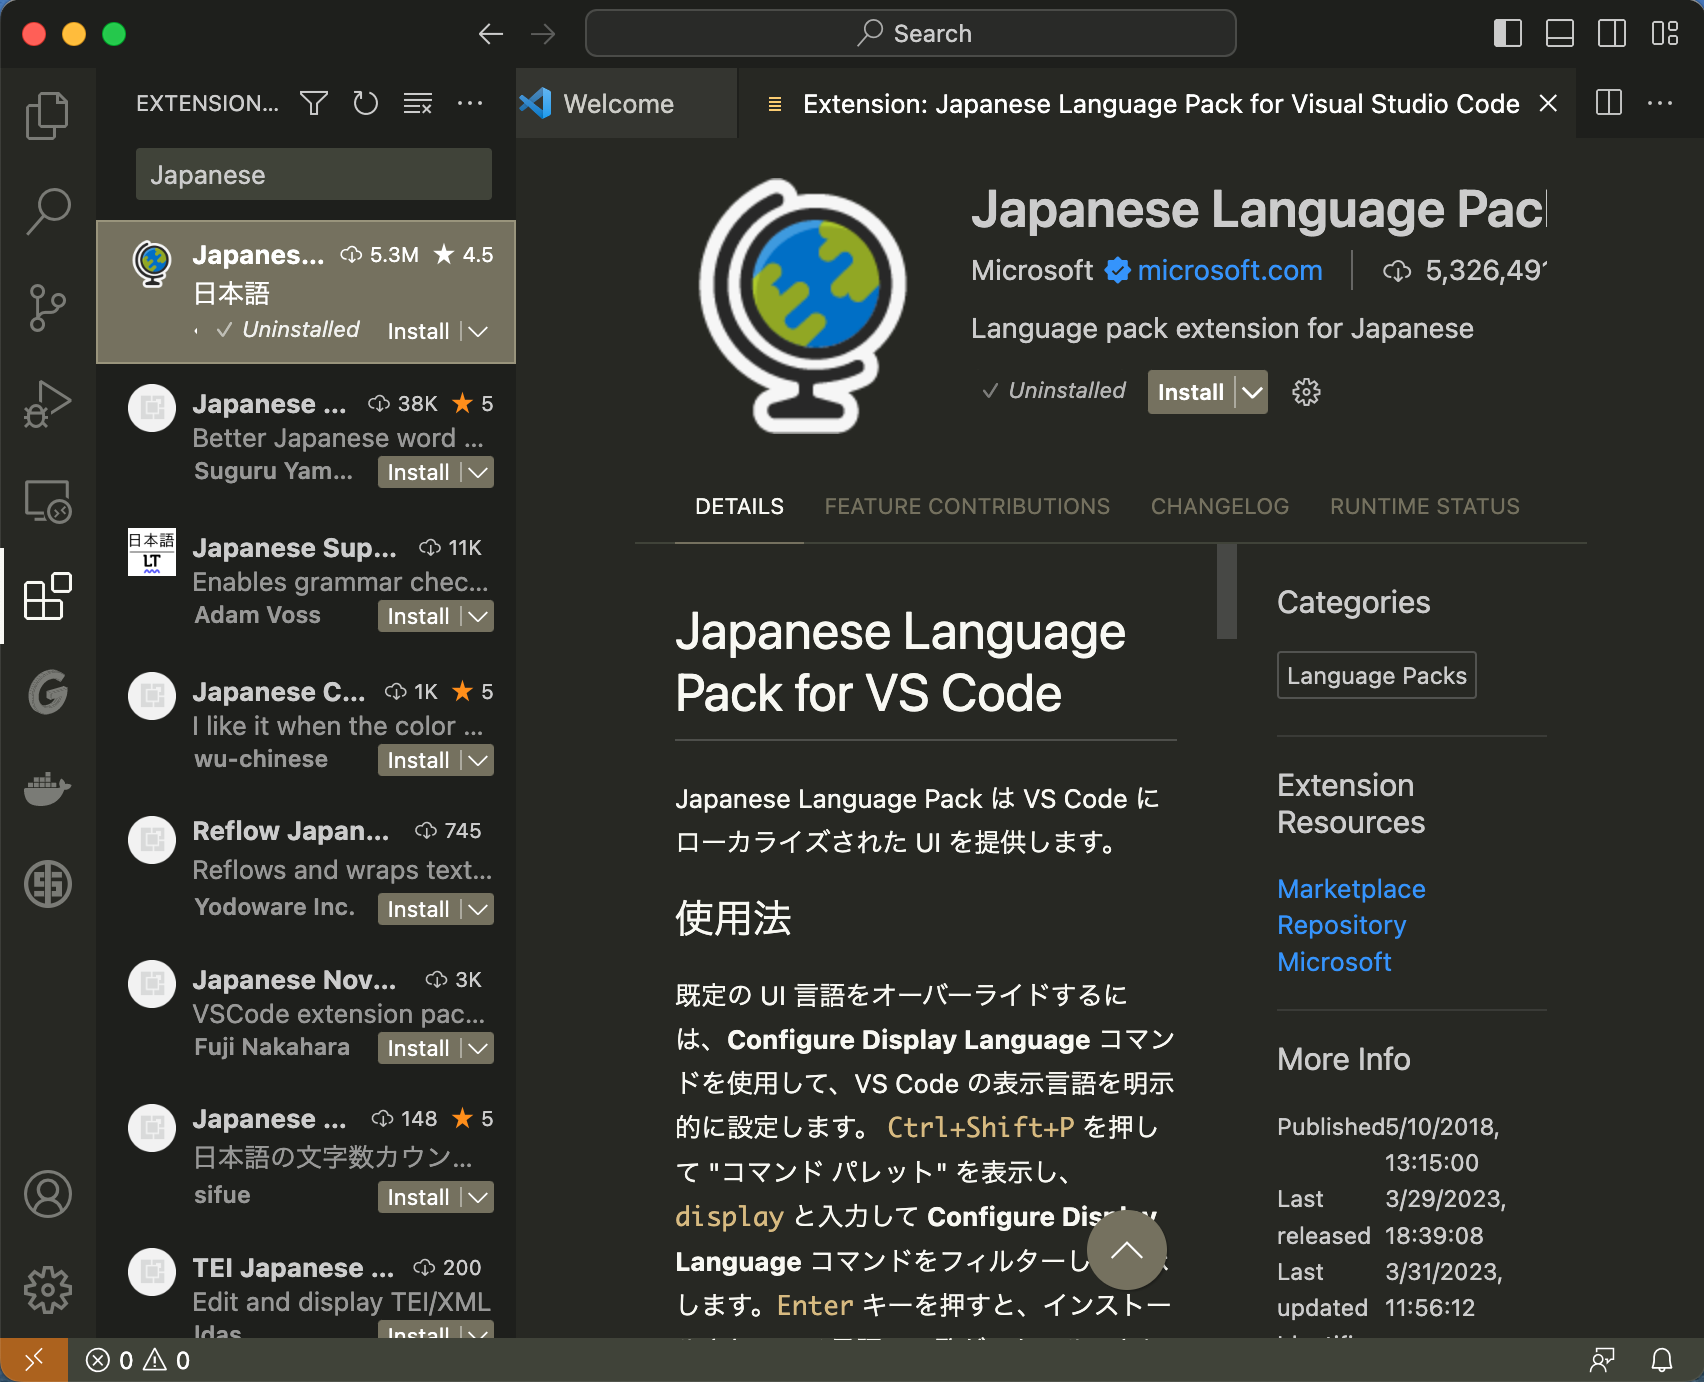
\includegraphics[height=7.5cm]{fig/VSCode2.png}
\end{figure}

上のナビゲーションのViewからCommand Paletteを選択して,検索窓を表示させます.そこにConfigure Display Languageと入力してReturnしましょう.jaを選択すると再起動を促されます.再起動すると日本語表示に変わります.\\
ただ,eduの端末だと日本語表示に切り替わらない可能性があります.

\begin{figure}[H]
  \centering
  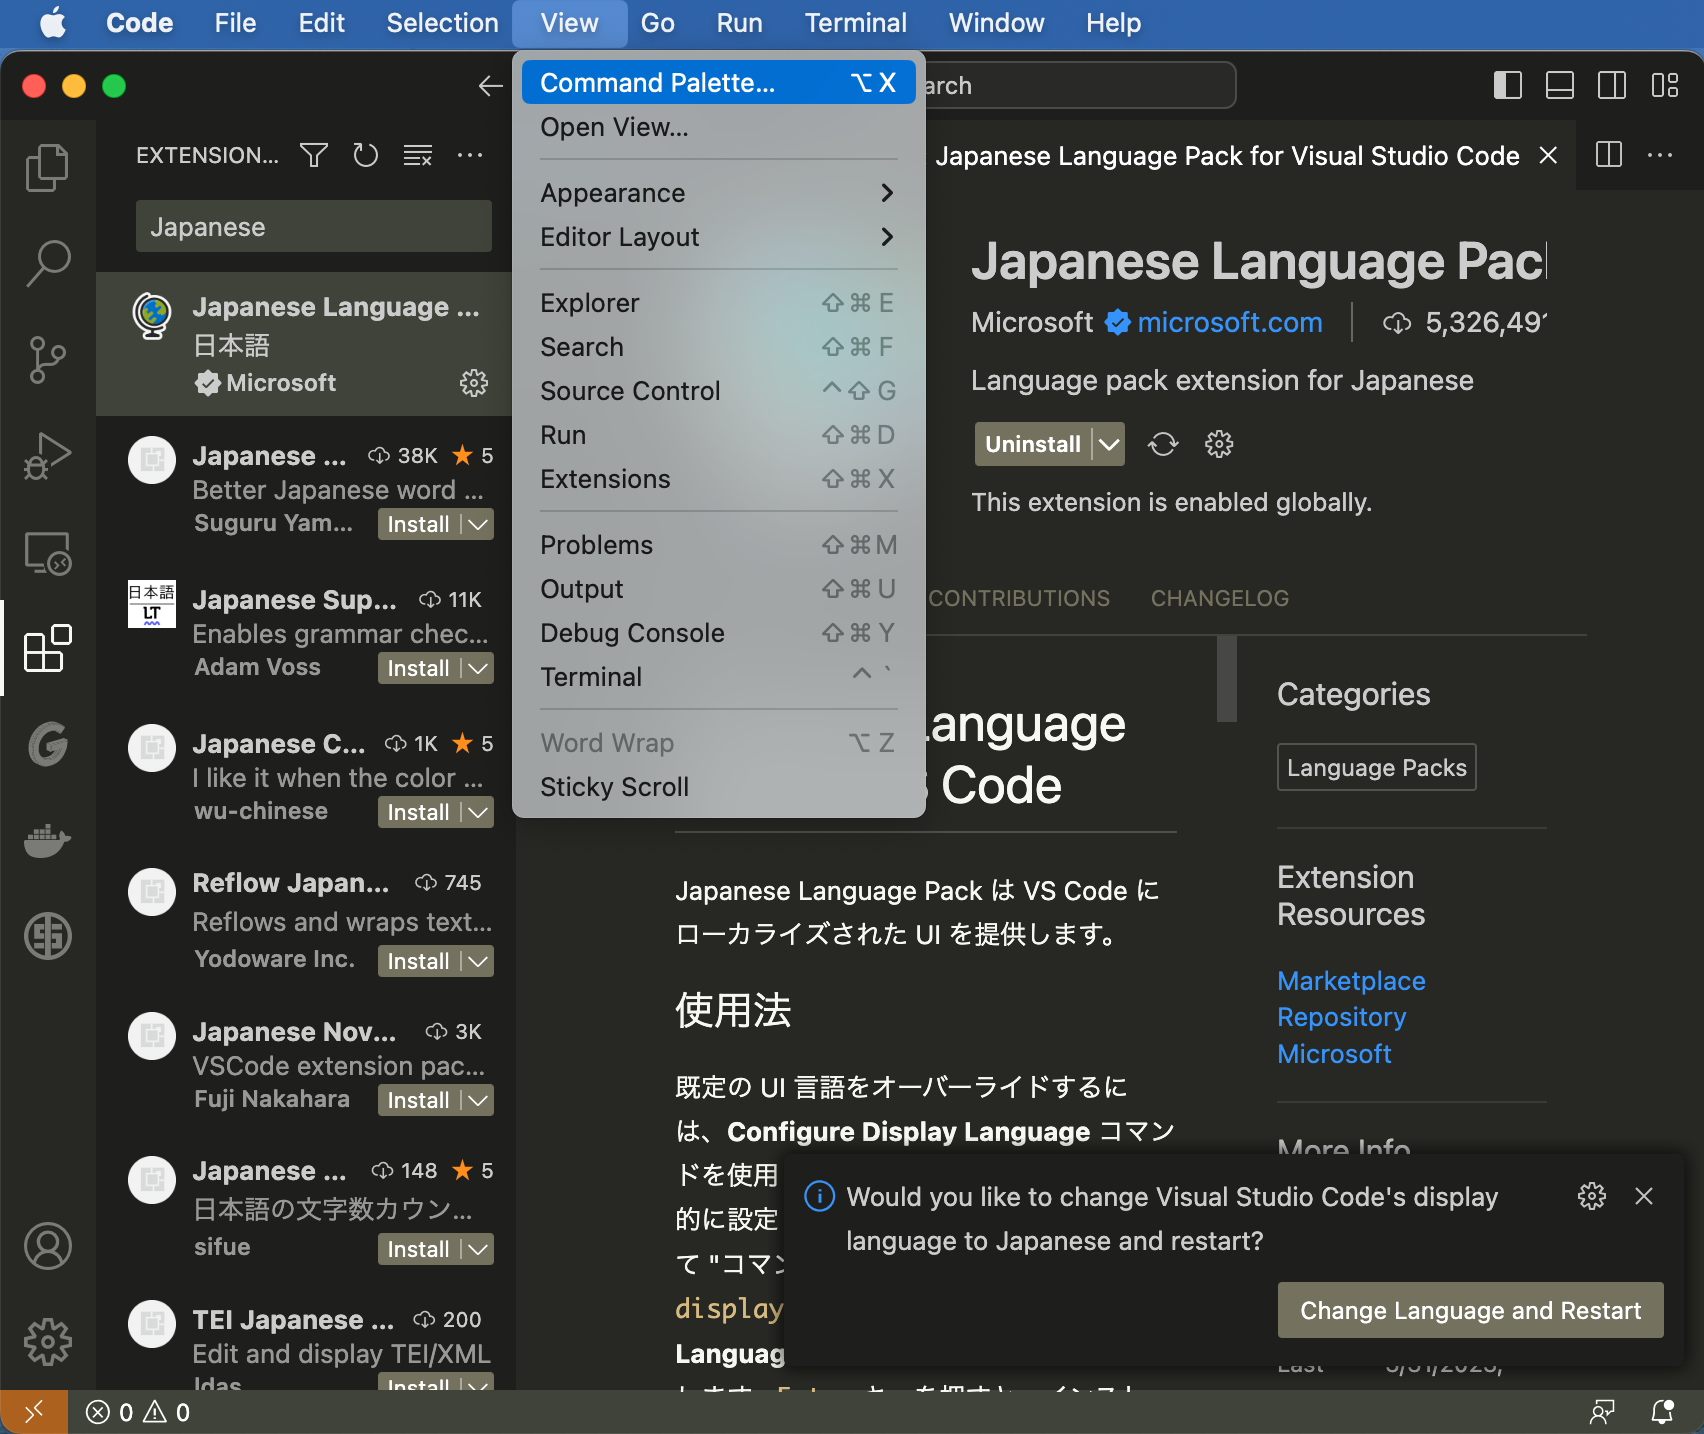
\includegraphics[height=7.5cm]{fig/VSCode3.png}
\end{figure}
\begin{figure}[H]
  \centering
  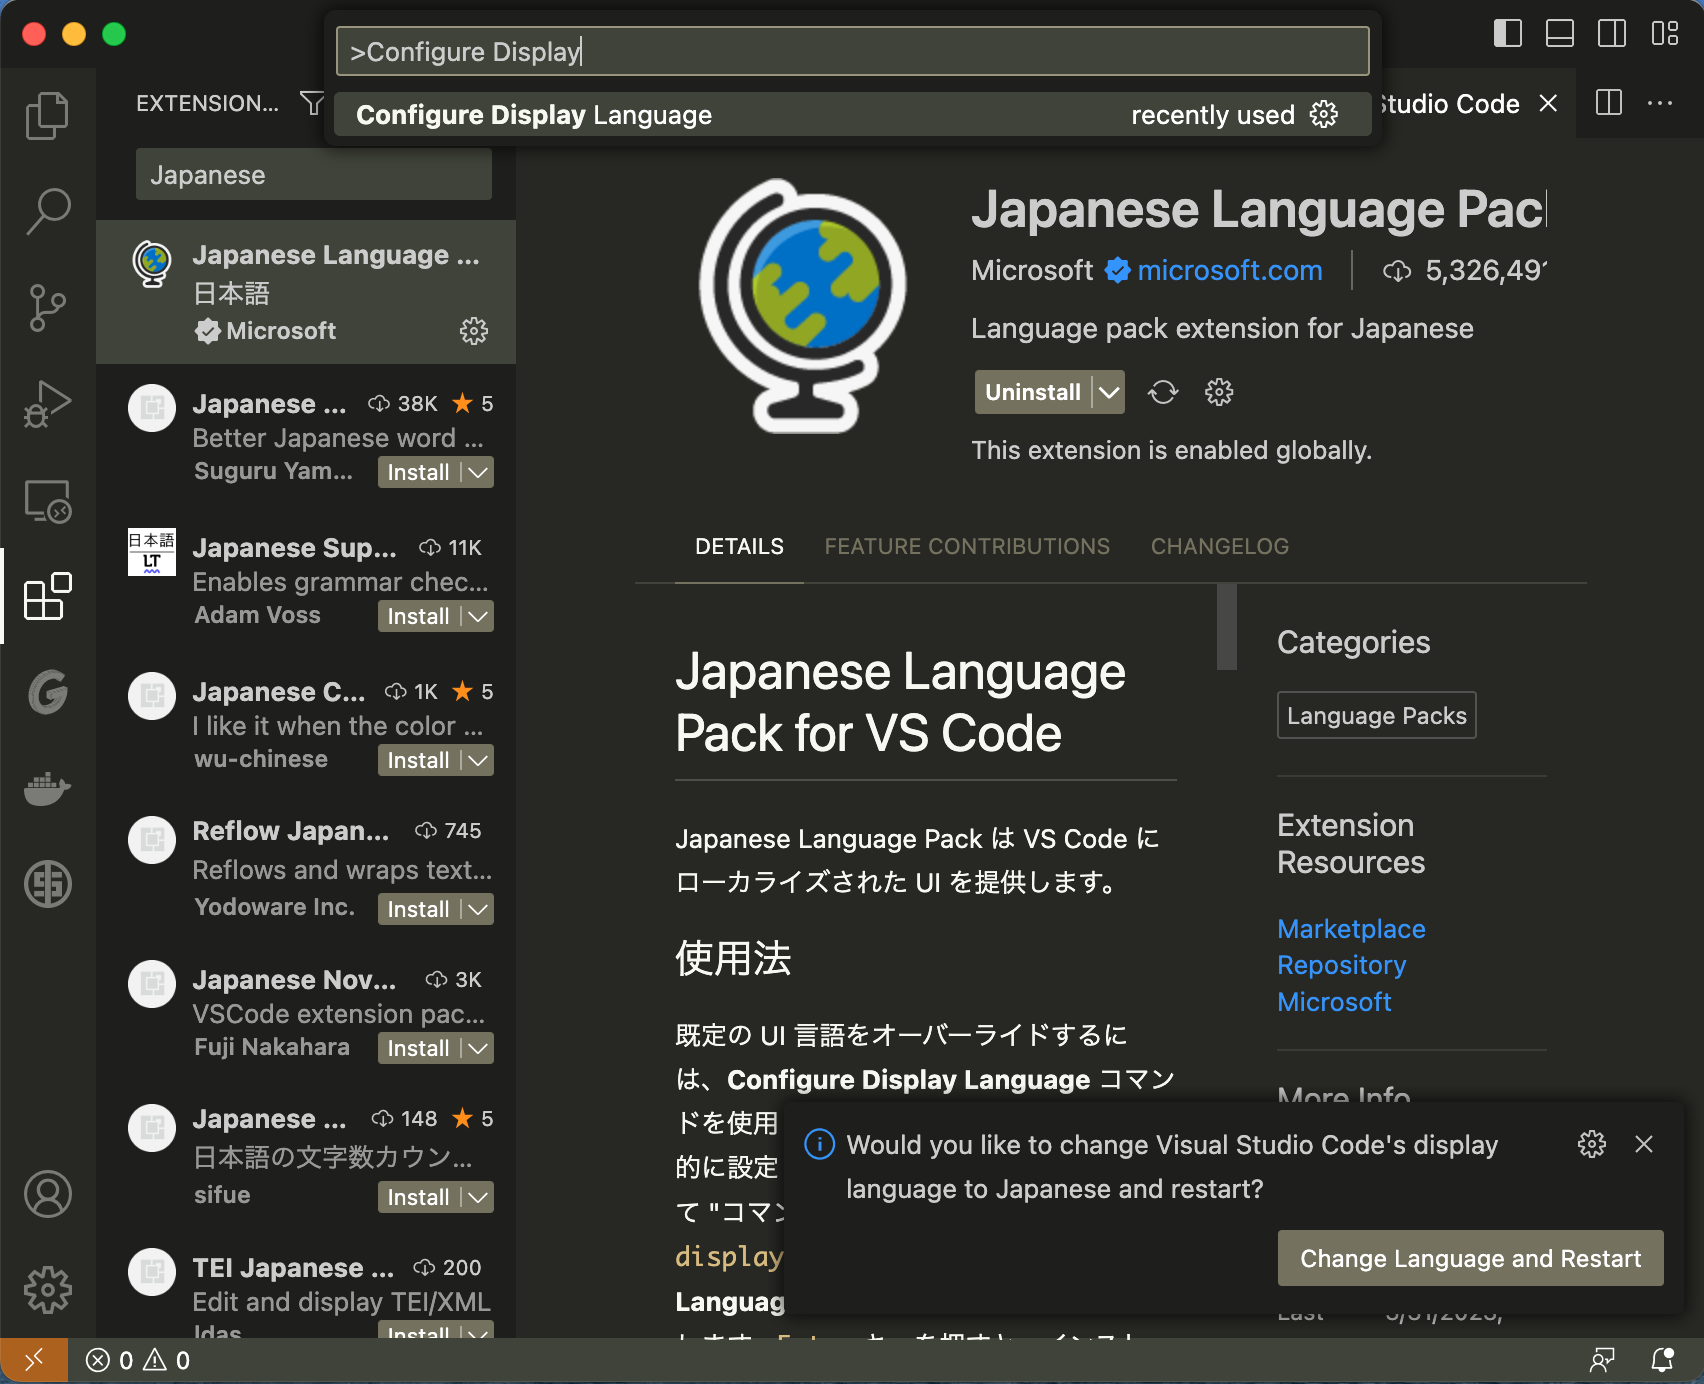
\includegraphics[height=7.5cm]{fig/VSCode4.png}
\end{figure}

\subsubsection{ファイルの操作}
上のナビゲーションのFile(ファイル)から開くことができます.ディレクトリを開いて複数ファイルを開くこともできます.

\subsubsection{VSCode上のターミナル}
上のナビゲーションのTerminal(ターミナル)からVSCode上でターミナルを開くことができます.開くと以下のような画面になります.コードを編集していてシームレスにコマンドを実行することができるため,便利です.

\begin{figure}[H]
  \centering
  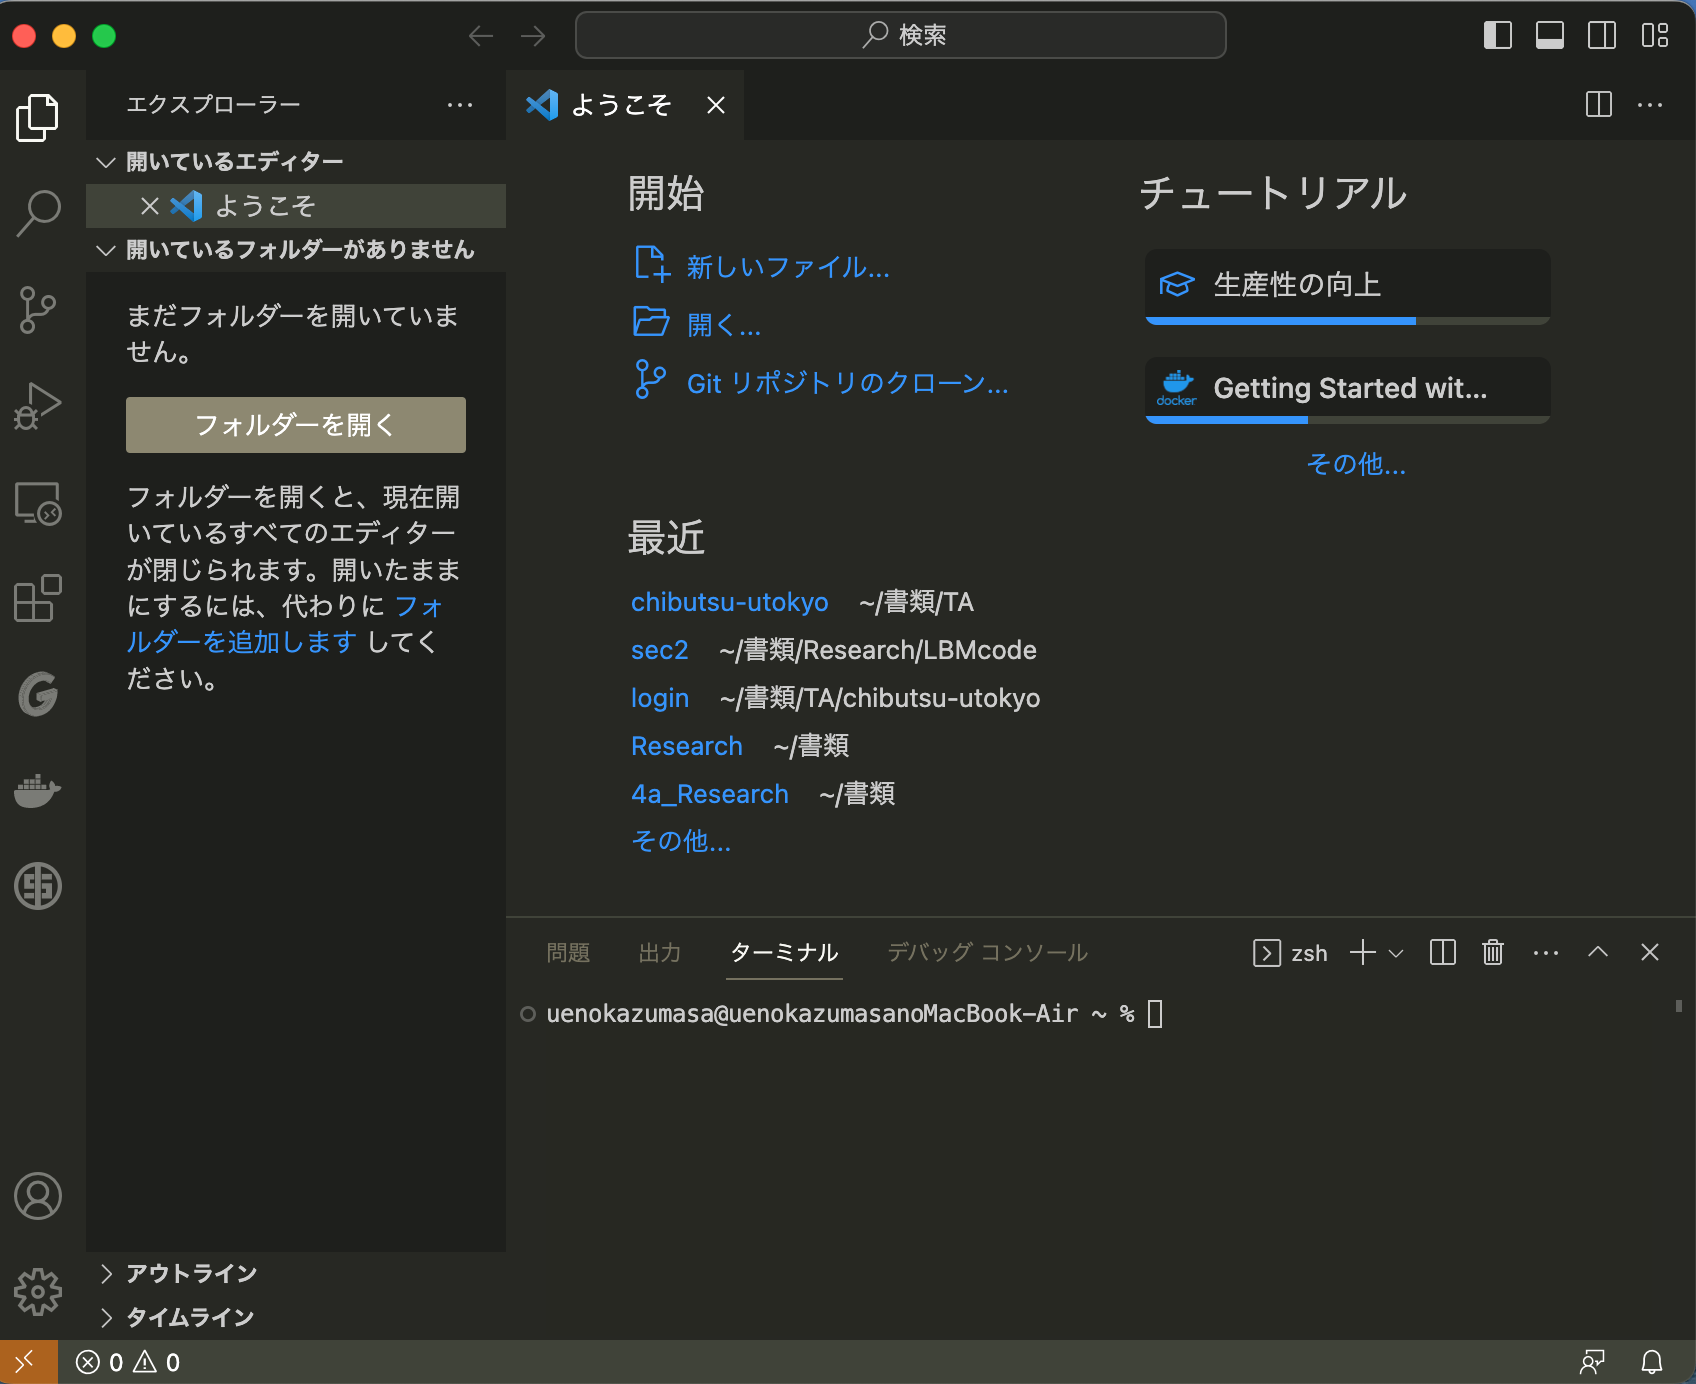
\includegraphics[height=7.5cm]{fig/VSCode6.png}
\end{figure}


\subsubsection{参考になりそうなページ}
\noindent
公式サイト(\url{https://code.visualstudio.com/})\\
Visual Studio Codeの使い方(\url{https://www.javadrive.jp/vscode/})\\
codeコマンドを使用可能にする(\url{https://qiita.com/P-man\_Brown/items/b18f31e3bb98b08ff31b})\\


\section{課題}
ここまででテキストエディタの基本的な使い方を学びましたので,関連する課題を出します.

お好みのテキストエディタで簡単な{\bf 自己紹介文}(特に,現段階で固体地球科学,大気海洋科学,宇宙惑星科学のどの分野に興味があるのか・{\bf 興味のある地球惑星科学的な現象}(例:地震,プラズマ,火山噴火,エルニーニョ,オーロラ,氷床変動,ハリケーン,竜巻,etc...))と{\bf 本日の演習の感想}を記載したファイルを作ってください.悩み事や演習に関係のない質問なども自由に書いてもらって構いません.
自己紹介文の書式は特に指定しませんが,最低限{\bf 名前}と{\bf アカウント名}は載せてください.ファイル名は{\bf 「s2326??\_1st.txt」}としてください.

ファイルが作成できたら,メールに添付して
\begin{center}
{\bf{上野(kazumasa-e67@eps.s.u-tokyo.ac.jp)}}
\end{center}
に送ってください.
% 締め切りは{\bf \underline{2019年4月15日(月)13時(JST)}}とします.

メールの件名は 
\begin{center}
{\bf{Geoph\_Emacs\_s2326**}}\\
\end{center}
としてください.この書式は必ず守ってください.

\section{ネットワーク}
次のテーマは,地物計算機室の{\bf マシン構成}を知ること,{\bf リモートマシン}(目の前にないマシン)に{\bf ネットワーク経由でアクセス}すること,ネットワークを使う上で重要な{\bf セキュリティ}を学ぶことです.

リモートマシンを使ったり,複数のマシン間でファイルをコピーしたりと,ネットワークに関する知識は皆さんがこれから研究を進めていく上で不可欠なものです.大学院に進学すると,研究室の{\bf ネットワーク管理}を任されたりするので,そのためにも今回の内容はよく理解しておいてください.

\vspace{1em}

ネットワークは非常に便利なものですが,自分ひとりのものではありません.当然のこと
ながら,ネットワークを利用する上でのマナーやセキュリティに関する知識も非常に重要になってきます.セキュリティというナイーブな問題を含むのでお説教じみた話もありますが,宜しくお願いします.

また,{\bf テキストの内容すべてを演習時間内に説明することはできない}ので,各自でよく読んでおくようにしてください.不明な点については,インターネット上にいろいろと知識や情報が載っているので,気になる用語はまず{\bf 検索}してみましょう.{\bf 主体的に調べようとすること}が何よりも{\bf 向上への近道}です.様々なエラー(コマンド上のエラーやプログラムする際のエラーなど)についても,とりあえず{\bf エラーメッセージを丸ごとGoogle検索にかけて解決}できることも多くあります.{\bf 今あなたが困っていることは,きっと誰かが一度は困ったことがあるのですから.}

% \subsection{用語}
\subsection{プロトコル(protocol)}
プロトコルとはネットワークを介して通信する際の手順や仕様を定めた規約のことで,通常
「通信規約」などと訳されます.以下は代表的なプロトコルの例です.

\begin{itemize}
\item TCP / IP (Transmission Control Protocol / Internet Protocol)\\
データをパケットに分けて送信します.UNIXワークステーションやインターネットにおける標準のプロトコルです.
\item Telnet (Telecommunication network)\\
仮想端末へのアクセスプロトコルです.
\item SMTP (Simple Mail Transfer Protocol)\\
電子メールの送信用に使われるプロトコルです.
\item FTP (File Transfer Protocol)\\
ファイルを転送するためのプロトコルです.
\item HTTP (HyperText Transfer Protocol)\\
Webページを表示するための通信などに使われるプロトコルです.
\end{itemize}

\subsection{ドメイン名とIPアドレス}
ネットワーク上でマシンを識別するために,ネットワークに接続されている各マシンには{\bf IPアドレス}という番号がつけられます.たとえば,演習室にある{\bf dover}というマシンのIPアドレスは“{\bf 133.11.229.15}”です.ただ,この形式は人間には覚えにくく使いにくいものです.そこで,DNS(\textbf{D}omain \textbf{N}ame \textbf{S}ystem)という仕組みを用いて,人間が理解しやすいように文字列で書かれた{\bf ドメイン名}とよばれるものを1つ1つのIPアドレスに対応させています.例えば,“{\bf 133.11.229.15}”に対応するドメイン名は“{\bf dover.eps.s.u-tokyo.ac.jp}”です.ここで“dover.eps.s.u-tokyo.ac.jp”は,“{\bf eps.s.u-tokyo.ac.jp}”にある“{\bf dover}”というマシンですよ,という意味です.

IPアドレスの種類には,世界中で通用するグローバルIPアドレスと,ローカルなネットワーク内(例えば家の中のLAN)だけで通用するプライベートIPアドレスとがあります.\footnote{1990年代初頭,日本でグローバルIPアドレスの割り当てが始まった頃,当時はIPアドレスが潤沢にあったので,東大には133.11.0.0から133.11.255.255までの65536個(!)ものIPアドレスが割り当てられました.IPv4アドレスの枯渇が世界的な問題になっている現在でも,東大内ではインターネットに公開しないeduなどのコンピュータやプリンターにまでグローバルIPアドレスを「贅沢に」割り振って使っていますが,これは東大が日本のインターネットに黎明期から関わってきたという歴史を感じさせるものです.}

\begin{itembox}[l]{\textbf{練習問題1}}
\url{http://133.11.228.207}をブラウザで開いてください.
\end{itembox}

\subsection{ファイアウォール}
組織内部のローカルなネットワークへの外部からの侵入や攻撃を防ぐ目的で設置されるホスト
やルータのシステムを{\bf ファイアウォール}と呼びます.ファイアウォールは組織内外からの通信要求を受け取り,それらを選択的に通過させます.こうすることで,内部のネットワークには必要
なサービスを提供しながら外部からの怪しい要求を拒否してセキュリティを確保します.

地惑ネットワークの一般の端末には外部からは接続できないようになっています.例外として,{\bf dover}に限り外部から接続できるようになっています(ただし{\bf SSH接続}に限る).そのため,外部から演習室のネットワークにアクセスするときには,{\bf まずdoverにSSHでアクセスして,そこから演習室内部のマシンに入る},という手順を踏む必要があります.ただし,{\bf www-geoph}に置いたファイルについてはWeb上に公開することができます.やり方は後で説明します.


\section{セキュリティ・マナー}
\subsection{パスワード}
パスワードの管理はセキュリティの基本です.
パスワードが漏洩すると,自分に被害があるばかりで なく同じシステムを使っている他の人にも被害が及びます.
パスワードの管理は厳重に行い,他人に知られることのないよう,十分気をつけてください(教えるとかは論外です.サンシャイン池崎という自分の預金残高とキャッシュカードの暗証番号を大声で叫ぶ芸人がいたそうですが,パスワード管理の面からは非常にナンセンスです).
パスワードを人に知られないために個人情報(名前や生年月日など)から推測できないような複雑なパスワードをつけましょう.
パスワードをメモ帳に書く,携帯電話内に記録する,写真に撮るなどの行為もNGです.
また,人が後ろにいるときにパスワードを入力するのも危険な行為なので注意しましょう.セキュリティに関しては性悪説で考えるクセを養いましょう.
\begin{itemize}
\item 良いパスワードの例:Hm5UniT7 ($\leftarrow$ここに記載されているからといって使用してはいけませんよ,受講者全員に筒抜けです!)
\item 悪いパスワードの例:
	\begin{itemize}
	\item Goto ... 名前
	\item Otog ... 名前の逆つづり
	\item Goto0410 ... 名前と誕生日
	\item g0t0 ... oを0にしただけ
	\end{itemize}
\end{itemize}

兎にも角にも,セキュアでないと思われるパスワードの付け方はやめましょう.

ソフト的にセキュリティの穴を埋めることはもちろん重要です.
しかし,人為的な理由により穴ができ,またそこを足がかりにシステムが攻撃を受けるというのは,よくあるパターンです.
システムの安全を守るためには,計算機管理者だけが意識していても不十分なのです.
一人一人のユーザの心がけが,皆さんのネットワークを守ります.

\subsection{教育・研究機関のネットワークを利用する上での注意点}
各ネットワークには利用に際して守るべきルール(User Access Policy)があります.
geophネットワークは東京大学という教育・研究機関のネットワークの一部ですから,
利用条件は教育・研究目的であることが前提で,大学のネットワークを用いて営利活動をすることなどは禁止されています.
また,ハードディスクやメモリなどの資源を一部のユーザが独占することもあってはなりません.
 
要は,「{\bf 人に迷惑をかけないようにしよう}」ということです.
個人レベルでセキュリティに気をつけるというのも,「人に迷惑をかけない」ことの一部であります.
たとえば,あなたのパスワードが漏洩したら,
それを悪用しようと考える人はあなたの名前を騙ってgeophネットワークの資源を破壊してしまうかもしれません.
他のネットワークを攻撃するための足がかりにされるということも十分ありえます.
あなたが利用するPCがウイルスに感染した場合,あなたが被害を受けるだけでは済まないことになります.
ネットワーク上では,被害者が即加害者となってしまいますので,しつこいようですがセキュリティ管理にはよくよく注意をはらってください.
小さなつもりの穴から水が漏れて,どんどん穴が広がっていくということはネットワークでは十分起こりうることなのです.
また,学内の端末で行われた通信のログは監視されています.
ファイル交換のP2Pソフトを使ったりすると厳しい措置がとられるので注意してください.

\newpage
\subsection{EPSのセキュリティ・ポリシー}
EPS(地球惑星科学専攻)では以下のような通信制限を定め,セキュリティを確保しています. ホストを大雑把に
\begin{itemize}
\item サーバ類
\item 外からの通信をSSHに限り許すもの
\item 外向きの通信のみできるもの
\item 外との通信を一切しないもの
\item その他
\end{itemize}
に分け,それぞれの類別によって必要な部分だけ外部から見えるようにルータで設定しています.
このような通信制限により,侵入者がセキュリティの穴を探すことは難しくなっています.
しかし,いったん侵入されるとフィルタリングはそもそも無意味になってしまいます.
そこで,以下のようなことが推奨されています.
\begin{itemize}
\item ネットワークが盗聴されていてもパスワードが漏れないようTelnetでなくSSHを使う.
\item 盗聴されている恐れのあるところと学内とでは違うパスワードを使う.
\item NFSもexportする先を明示的に限定する.
\item 不要なアカウントは返却する.
\end{itemize}
詳細は\url{http://www.eps.s.u-tokyo.ac.jp/inside/network/security.html}を参照してください.

\section{UTokyo WiFi}
自分のノートパソコンを持ってきた場合,学内の建物では,
ほぼ全域で東京大学の無線LAN(UTokyo Wi-Fi)を使ってインターネットに接続することができます.SSIDは「0000UTokyo」です.
% ただし,利用するには「電子証明書」という鍵のようなもののインストールが必要で,
% そのためにはウェブから認証システムにログインしてからユーザ証明書をダウンロードする手順をとります.
% 認証システムへのログインアカウントについては,専攻のネットワーク管理者から配布されることになっていますが,システムは頻繁に変わります.最新の情報を下記のリンクから参照してください.

\begin{itemize}
\item 理学系研究科 情報システムチーム
\url{http://jimubu.adm.s.u-tokyo.ac.jp/public/index.php/Joho}

また,UTokyo Accountを所有している皆さんは,東京大学の全学無線LANサービスUTokyo WiFiも簡単に登録・利用することができます.

\item オンライン授業・Web会議ポータルサイトuteleconのUTokyo Wi-Fi 利用案内\\
\url{https://utelecon.adm.u-tokyo.ac.jp/utokyo_wifi}
 
 ※自分のパソコンなので自宅感覚で使ってしまいがちですが,無線LANであっても大学のネットワークです.学内の端末を使う場合と同じ注意を払ってください.
\end{itemize}

\newpage
\section{地物演習室(計算機室・559)の構成とネットワーク}
\subsection{サーバとクライアント}
演習室にあるマシンは以下の表に示す通りです.
\begin{table}[htb]
  \centering
  \begin{tabular}{|l|l|l|} \hline
    ドメイン名 & グローバルIPアドレス & 役割 \\ \hline
dover.eps.s.u-tokyo.ac.jp & 133.11.229.15 & 外部ネットワークログイン用SSHサーバ\\ \hline
sakura.eps.s.u-tokyo.ac.jp & 133.11.229.101 & 
\begin{tabular}{l}
ネットワークアカウント(LDAP)サーバ \\ 兼ファイル(NFS)サーバ 
\end{tabular} \\ \hline
www-geoph.eps.s.u-tokyo.ac.jp & 133.11.228.207 & Webサーバ \\ \hline
asano.eps.s.u-tokyo.ac.jp & 133.11.231.4 & 高速並列計算サーバ\\ \hline
edu\{01-35\}.eps.s.u-tokyo.ac.jp & 各端末に記載 & 学部生用のクライアント(Mac mini) \\ \hline
  \end{tabular}
\end{table}

これらのマシンは下図のようにつながっています.
\begin{figure}[htbp]
 \begin{center}
  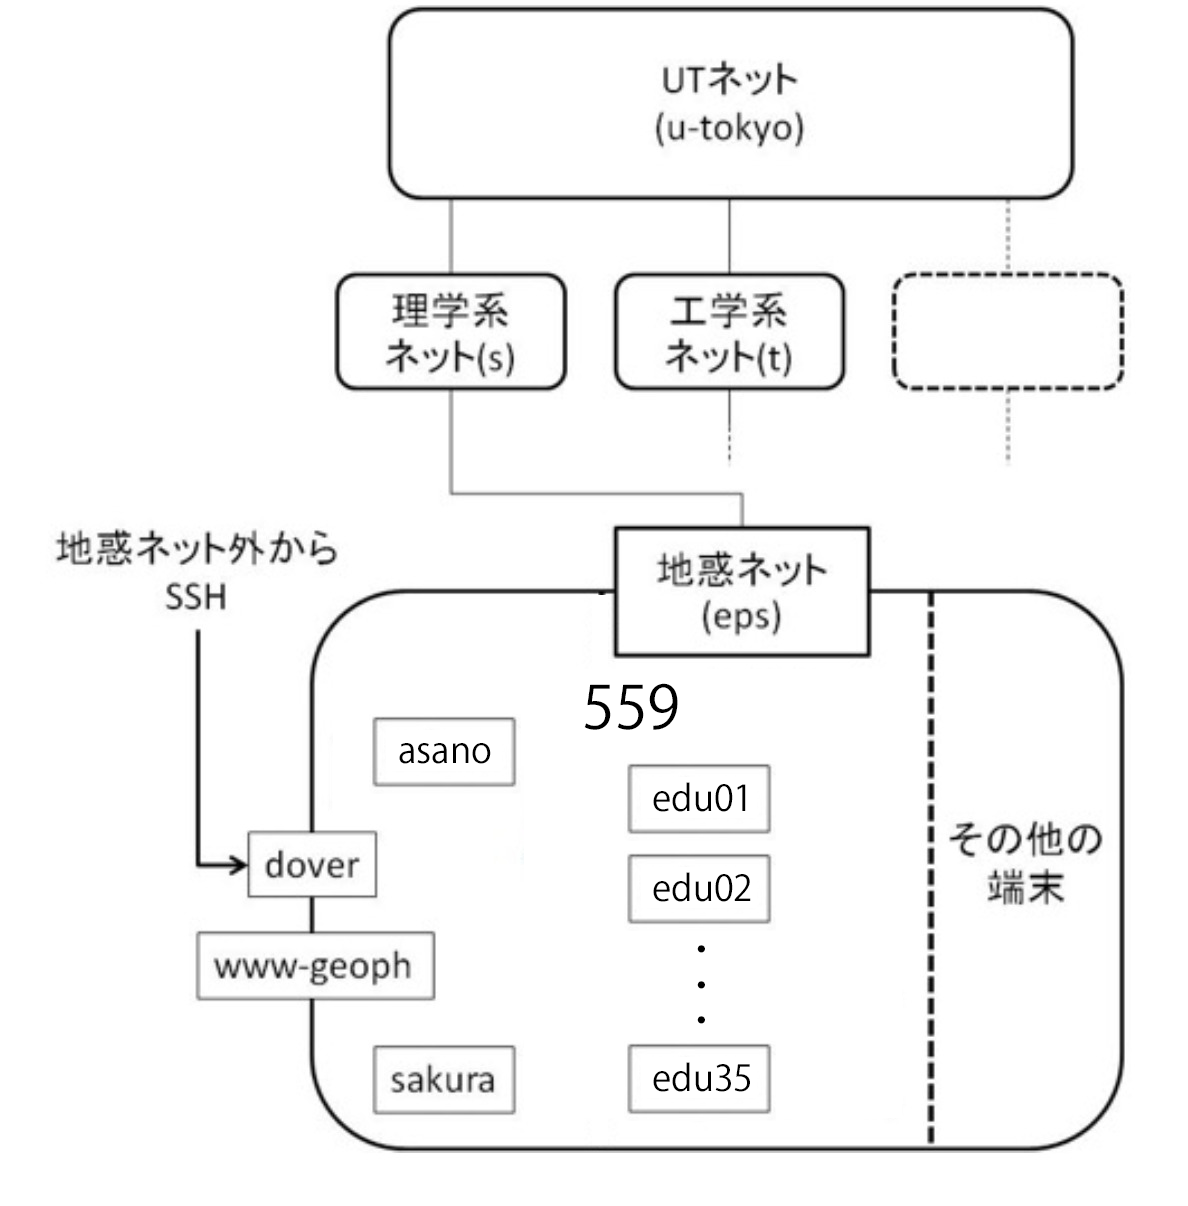
\includegraphics[width=10cm,pagebox=cropbox,clip]{fig/eps-net.png}
 \end{center}
 \label{fig:one}
\end{figure}

\subsubsection{doverの役割}
SSHサーバ:外のネットワークと地惑のネットワークをつなぐ.地惑ネット外(例えば図書館や自宅の端末)から計算機室内の端末を利用したければ,sshを用いてdoverを経由してログインする.

\subsubsection{www-geophの役割}
Webサーバ:Webページとして公開するデータを置く場所(やり方は後述).

\subsubsection{sakuraの役割}
% {\bf NIS}:Network   Information   Service  の略.ネットワーク上の複数のコンピュータ間でユーザ情報を共有するシステム.演習室のどの端末でも,同じユーザ名・パスワードでログインできるのはNISのおかげです.
\begin{itemize}
\item {\bf LDAP} \ 
Lightweight Directory Access Protocol の略.TCP/IPでディレクトリサービスを提供するためのプロトコル.これを用いてネットワーク上でアカウント情報を共有することができます.演習室のどの端末でも,同じユーザ名・パスワードでログインできるのはLDAPのおかげです.

\item {\bf NFS} \ 
Network File System の略.複数のホスト間でファイルを共有するシステムです.eduの/opt/mac・/home1・/home2はsakuraの/opt/mac・/home1・/home2を共有したものです.どの端末にログインしても同じファイルを編集できるのはNFSによるものです.

\item バックアップ \ 
毎週土曜日にバックアップを取っています.なにか大事なものを消してしまったときはここにとりに来ましょう(やり方は後述).
\end{itemize}

このようにsakuraの担っている役割のおかげで地物の計算機室は機能しています.もし普段使っている計算機にトラブルが起きて再起不能になっても,sakuraさえ無事であれば他の端末を使って同じ作業を続けられる,ということになります.

\subsubsection{asanoの役割}
数値シミュレーションなど重い計算をさせるための計算用サーバとして導入されました.
使い方は\href{http://www-geoph.eps.s.u-tokyo.ac.jp/~s162633/epp_computers/index.php?asano}{計算サーバasano}(地物の端末からのアクセス専用)に載せています.ちなみにこのHPはウェブサーバ {\bf www-geoph} で公開されているページです.

普通のPCより速く,並列計算もこなせるので,5月祭の準備・特別演習・趣味などで重い計算をする時に是非活用してください.


\subsection{遠隔ログイン(SSH)}
遠隔ログインを用いれば,リモートマシン(目の前にないマシン)を使うことができます.具体的な用途として,「{\bf 自宅から計算機室の端末にログインして演習で出題された課題に取り組む}」などが挙げられます.便利,というより今後時間のかかる課題に取り組む上で必須になる用途ですのでぜひ身につけましょう.
 
% \subsection{SSH}
通信を暗号化した遠隔ログイン方法として広く使われているのがSSH  (Secure SHell)です.やり方は以下の通りです.

SSHを利用してリモートホスト(遠隔地にあるサーバ)にログインするには,
\begin{verbatim}
$ ssh username@hostname
\end{verbatim}
とします.ホスト名の部分にはIPアドレスをそのまま書いても構いませんが,普通はドメイン名を入力します.例えば,
\begin{verbatim}
$ ssh s2326??@dover.eps.s.u-tokyo.ac.jp
\end{verbatim}
といった具合です.入力後,パスワードを聞かれたら入力してリターンしてください.

なお,ローカルホスト(本人の手元にある端末)とリモートホストとでユーザ名が一致している場合は,
\begin{verbatim}
$ ssh hostname
\end{verbatim}
とusernameを省略してもOKです.

初めてsshでログインするホストにアクセスしたときは,
\begin{Verbatim}[baselinestretch=0.5]
The authenticity host ‘dover (133.11.229.15)’ can’t be established.
DSA key fingerprint is cb:27:ec:3c:ff:02:f6:fc:9e:7b:39:80:e7:0f:9e:bf.
Are you sure you want to continue connecting (yes/no) ?
\end{Verbatim}
などとたずねられますので,
\begin{verbatim}
yes 
\end{verbatim}
と打ってください.

リモートホストで作業が終わってログアウトする際には,
\begin{verbatim}
$ exit
\end{verbatim}
と打てばもとのローカルホストでの作業に戻れます.

ここで大事なことですが,sshの後に「-X」(大文字であることに注意!)というオプションをつけないと,リモートホストでウィンドウを開く系の作業ができません.このオプションをつけることで,X window system (ウィンドウを開いてくれるシステム)も自動的に転送されるようになり,
リモートで開いたウィンドウがローカルで見えて操作できるようになるのです\footnote{たまに{\bf -X}をつけてもうまくいかない場合があります.
その場合は{\bf -XY}とすると解決することがあります.}.
% 試しに「-X」なしでログインしてから,
% \begin{verbatim}
% $ emacs &
% \end{verbatim}
% と入力してEmacsを起動しようとしてみてください.新しいウィンドウを開けずに,エラーとなってしまうはずです
% \footnote{{\bf \$ emacs -nw \&}のように{\bf nw}オプションをつけると,現在のシェル上にEmacsが起動するためエラーにはなりません.}.その他のアプリケーションについても,ウィンドウを開くことができないはずです.

なお,この機能を利用するためにはローカルのマシンにXサーバという種類のソフトがインストールされている必要があります.もちろん計算機室の端末({\bf edu})のマシンでしたら既にインストールされているので問題ありませんが,自宅からリモートログインする際には注意してください(後述).\\

SSHについては、UNIX第2回の授業で詳しく説明します。

\vspace{1em}

\begin{itembox}[l]{\textbf{練習問題2}}
doverにSSHでログインしてログアウトしてください.
\end{itembox}

% \subsection{自宅からSSHをするには(※この節は演習の時間中は読み飛ばして構いません)}
% 自宅のパソコンからでも,インターネットに接続されていれば,今みなさんがやっているのと同じように,演習室にリモートログインして作業ができます.これは非常に便利です.ただし,予めローカルホストとなる自宅のパソコンにSSH接続に必要なソフトウェアをインストールする必要がありますので,使用しているOSに合わせて適切な環境設定をしましょう.

% \subsubsection{Windowsの場合}
% Windowsでは,デフォルトではSSHを使うことはできません\footnote{Windows10では2016年夏のアップデートでbashが使えるようになる予定です.そのためデフォルトでSSHも使えるようになると思われます.}.SSHを使うには,PuTTYというTelnet/SSHクライアントソフトが便利です.他にもTeraTermやPoderosaなど色々ありますが,詳しくは調べてみてください.別ウィンドウを立ち上げる作業もしたいのであれば,XmingなどのXサーバも入れる必要があります.あるいは,CygwinというWindows上でUNIXライクな環境を再現するソフトをインストールすれば(少し手間ですが),これらの環境がまとめて揃います.この他に,VMwareなどの仮想マシンにUbuntuを乗せる方法が手っ取り早いかもしれません.

% \subsubsection{Macの場合}
% Macの場合\footnote{他のUNIX/Linux系OSの場合も同様です.}には,ターミナルからそのままSSHができます.XQuartzをインストールすることで,別ウインドウを立ち上げる作業もできます.
% この時Mac上で \verb|~/.ssh/config| というファイルを作成し,
% \begin{Verbatim}[baselinestretch=0.5]
% Host dover
%         HostName dover.eps.s.u-tokyo.ac.jp
%         User s192601

% Host edu16
%         HostName edu01.eps.s.u-tokyo.ac.jp
%         User s192601
%         ProxyCommand ssh -X dover nc %h %p

% Host www-geoph
%         HostName www-geoph.eps.s.u-tokyo.ac.jp
%         User s192601
%         ProxyCommand ssh -X dover nc %h %p
% \end{Verbatim}
% のように記述しておくと便利です.こうしておけば
% \begin{verbatim}
% $ ssh -X s182601@dover.eps.s.u-tokyo.ac.jp
% \end{verbatim}
% とわざわざ入力しなくても
% \begin{verbatim}
% $ ssh -X dover
% \end{verbatim}
% と入力するだけで済むようになります.
% またeduやwww-geophにログインする場合もdoverに一旦SSHする必要はなく,直接
% \begin{verbatim}
% $ ssh -X edu01
% \end{verbatim}
% とするだけで済みます.SCP(後述)やSSHFS\footnote{本テキストでは説明しません.リモートマシン上のファイルをローカルのファイルと同じように扱えるため便利なので中〜上級者は使ってみてください.}にも有効なのでぜひ設定しましょう.

% なおMacからeduにログインした場合に,日本語が文字化けすることがあります.ログイン後
% \begin{verbatim}
% $ export LANG=ja_JP.UTF-8
% \end{verbatim}
% とすることで解決するかもしれません.

% \section{ファイル転送}
% 遠隔ログインを使うようになると,ただログインするだけでなく,ファイルの転送もしたくなります.

% \subsection{SCP}
% ファイルの転送を暗号化するには,SCP (Secure CoPy)  を用います.SSHを利用して通信を行う方式なのでセキュアです.doverや演習室の端末と自分のパソコン間でファイルをやり取りする場合にはこれを使うことになるので,使用頻度はかなり高いと思います.使い方は以下の通りです.

% ローカルからリモートにファイルを送る場合には
% \begin{verbatim}
% $ scp filename1 [username@]hostname:filename2
% \end{verbatim}
% \verb|[username@]| となっているのは,ユーザ名がローカルとリモートで同じ場合に \verb|username@| を省略できるということで,SSHの時と同様です.例えば,手元にあるレポート課題をdoverに送りたい時は
% \begin{verbatim}
% $ scp report.pdf dover.eps.s.u-tokyo.ac.jp:enshu_report.pdf
% \end{verbatim}
% のようになります.

% 反対にリモートからローカルにファイルをとってくる場合には
% \begin{verbatim}
% $ scp [username@]hostname:filename1  filename2
% \end{verbatim}
% とします.さらに,-rオプションをつけると,ディレクトリのコピーもできます.recursive(再帰的)のrです. 

% いずれにせよ,「送るもの」を先に指定してから,「送り先」を指定します.

% \vspace{1em}

% \begin{itembox}[l]{\textbf{練習問題3}}
% \begin{enumerate}
% \item hoge1.datというファイルをdoverに送り,hoge2.datという名前で保存してください.
% \item 1.で送ったファイルをeduに取ってきて,hoge3.datという名前で保存してください.
% \end{enumerate}
% \end{itembox}

% \subsection{WGET}
% 例えば,http://www.eps.s.u-tokyo.ac.jp/access.htmlというファイルをダウンロードしたいとき,どのような方法があるでしょうか.
% GUIが好きであればFirefoxで右クリックして保存しても良いですが...CUIも使えるようにして欲しいですね....

% このファイルは地球惑星科学専攻の場所のアクセスマップです.この地惑専攻のウェブサーバには皆さんのアカウントはありませんからSCPは使えません.このような時は{\bf wget}コマンドを利用すると良いでしょう.wgetはWebからファイルをダウンロードするコマンドで,HTTP・HTTPS・FTPのプロトコルに対応しています.上の例だと,
% \begin{verbatim}
% $ wget http://www.eps.s.u-tokyo.ac.jp/access.html
% \end{verbatim}
% のようにして使います.
% “-x”オプションを用いれば,ディレクトリ構造を保ってダウンロードできます.つまり,
% \begin{verbatim}
% $ wget -x http://www.eps.s.u-tokyo.ac.jp/access.html
% \end{verbatim}
% とすると,カレントディレクトリに www.eps.s.u-tokyo.ac.jp というディレクトリができ,その中に access.html が保存されます.

% また,“-r”オプションを用いれば,指定したページに含まれるリンク先を再帰的に取得できます.

% \vspace{1em}

% \begin{itembox}[l]{\textbf{練習問題4}}
% \url{http://www-geoph.eps.s.u-tokyo.ac.jp/~s122621/kadai/index.html}とそのページに書かれているリンク先を全てダウンロードしてください.
% \end{itembox}

\subsection{eduの画面共有}
計算機室にあるeduをdover経由で画面共有して、自宅から操作することができます。
計算機演習や、学内からしか接続できないWebサイト(学内限定ページや学術誌の論文など)の閲覧に活用してください。

\subsubsection{Windowsの場合}
\begin{enumerate}
  \item VNCクライアント(UltraVNC Viewer)をダウンロードして、インストールします。
  \begin{center}
    \url{https://www.uvnc.com/downloads/ultravnc.html}
  \end{center}
  \item コマンドプロンプトを起動して\\
    \verb| ssh -L 4000:eduXX:5900 s2326XX@dover.eps.s.u-tokyo.ac.jp |  \\
  と入力します。eduは計算機室で自分が使うマシンを指定してください。
  \begin{figure}[H]
    \centering
    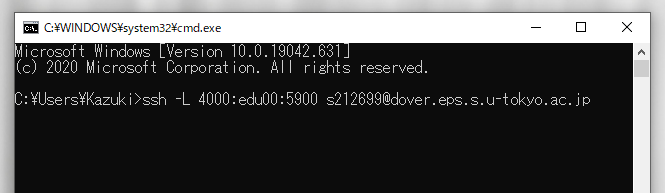
\includegraphics[height=4cm,pagebox=cropbox,clip]{fig/VNCWin1.png}
  \end{figure}
  \item UltraVNC Viewerを起動して、「localhost:4000」と入力し「Connect」をクリックします。
  \begin{figure}[H]
    \centering
    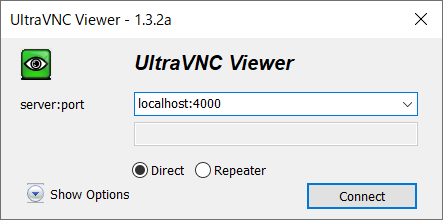
\includegraphics[height=4cm,pagebox=cropbox,clip]{fig/VNCWin2.png}
  \end{figure}
  \item パスワードを聞かれたら「geoph」と入力し「Log On」をクリックします。
  \begin{figure}[H]
    \centering
    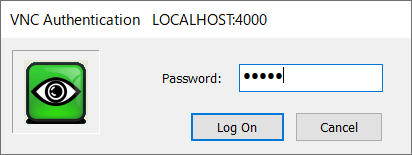
\includegraphics[height=3cm,pagebox=cropbox,clip]{fig/VNCWin3.png}
  \end{figure}
  \item eduのログイン画面が表示されます。自分のアカウントとパスワードを入力します。
  \begin{figure}[H]
    \centering
    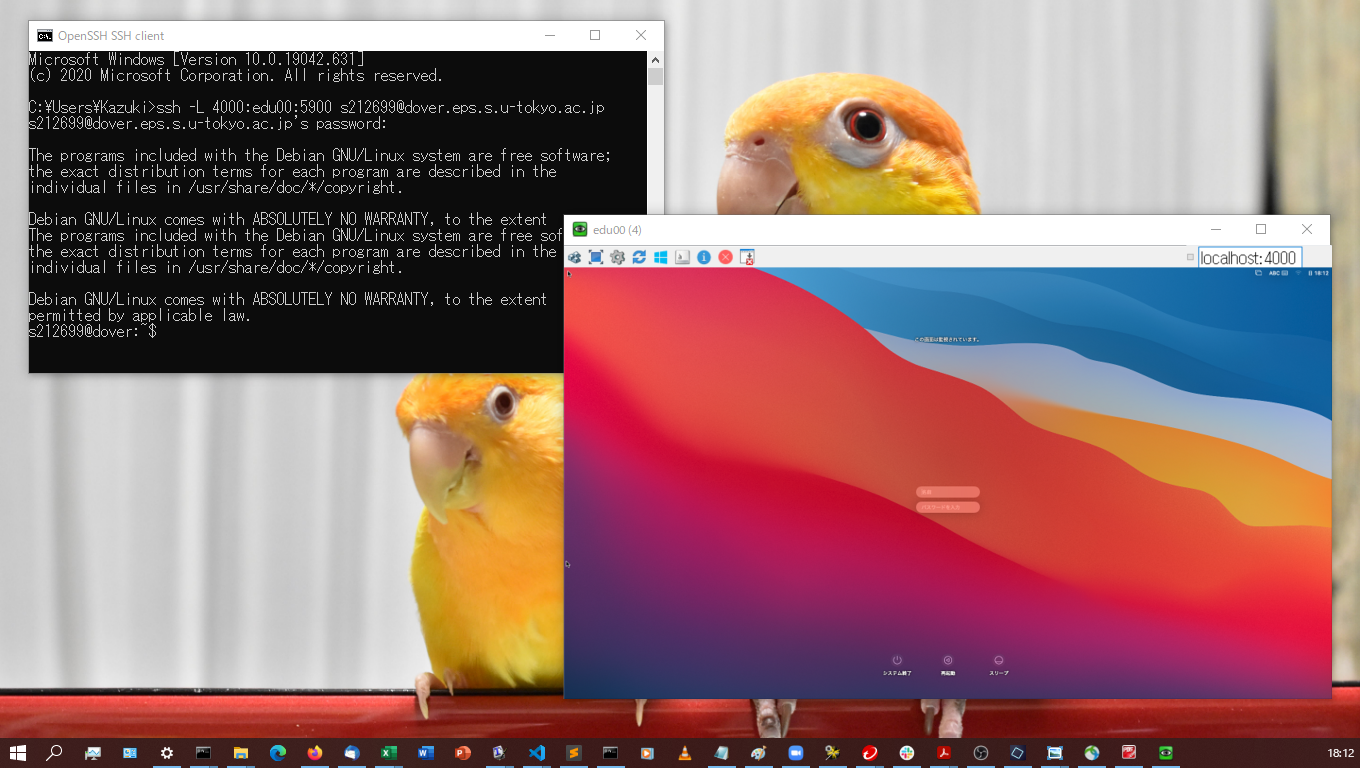
\includegraphics[height=7.5cm,pagebox=cropbox,clip]{fig/VNCWin4.png}
  \end{figure}
  \item eduのデスクトップが表示され、操作できます。
  \begin{figure}[H]
    \centering
    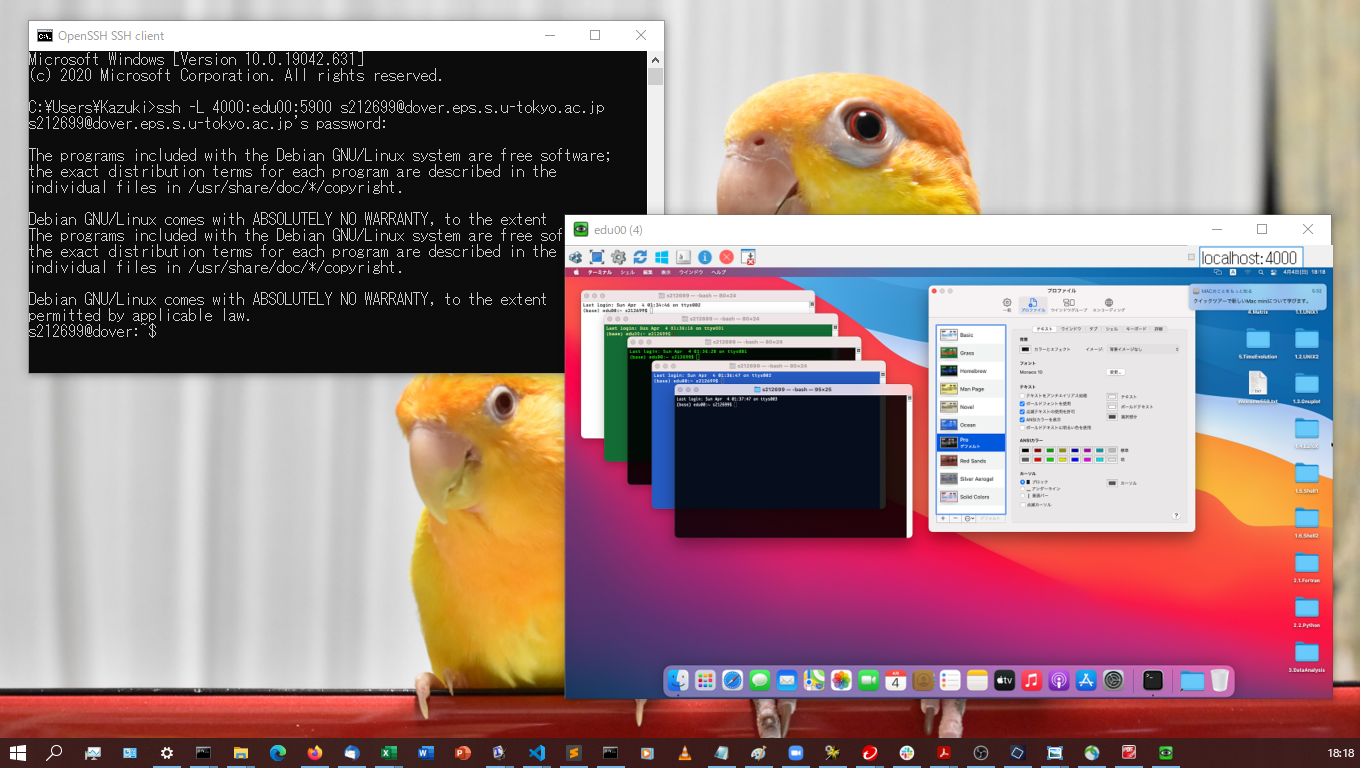
\includegraphics[height=7.5cm,pagebox=cropbox,clip]{fig/VNCWin5.png}
  \end{figure}
\end{enumerate}

\subsubsection{Macの場合}
\begin{enumerate}
  \item ターミナルを起動して\\
    \verb| ssh -L 4000:eduXX:5900 s2326XX@dover.eps.s.u-tokyo.ac.jp |  \\
  と入力します。eduは計算機室で自分が使うマシンを指定してください。
  \begin{figure}[H]
    \centering
    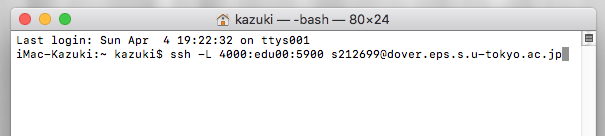
\includegraphics[height=3cm,pagebox=cropbox,clip]{fig/VNCMac1.png}
  \end{figure}

  \newpage
  \item デスクトップの何もないところをクリックし、「移動」→「サーバへ接続」の順にクリックします。
  \begin{figure}[H]
    \centering
    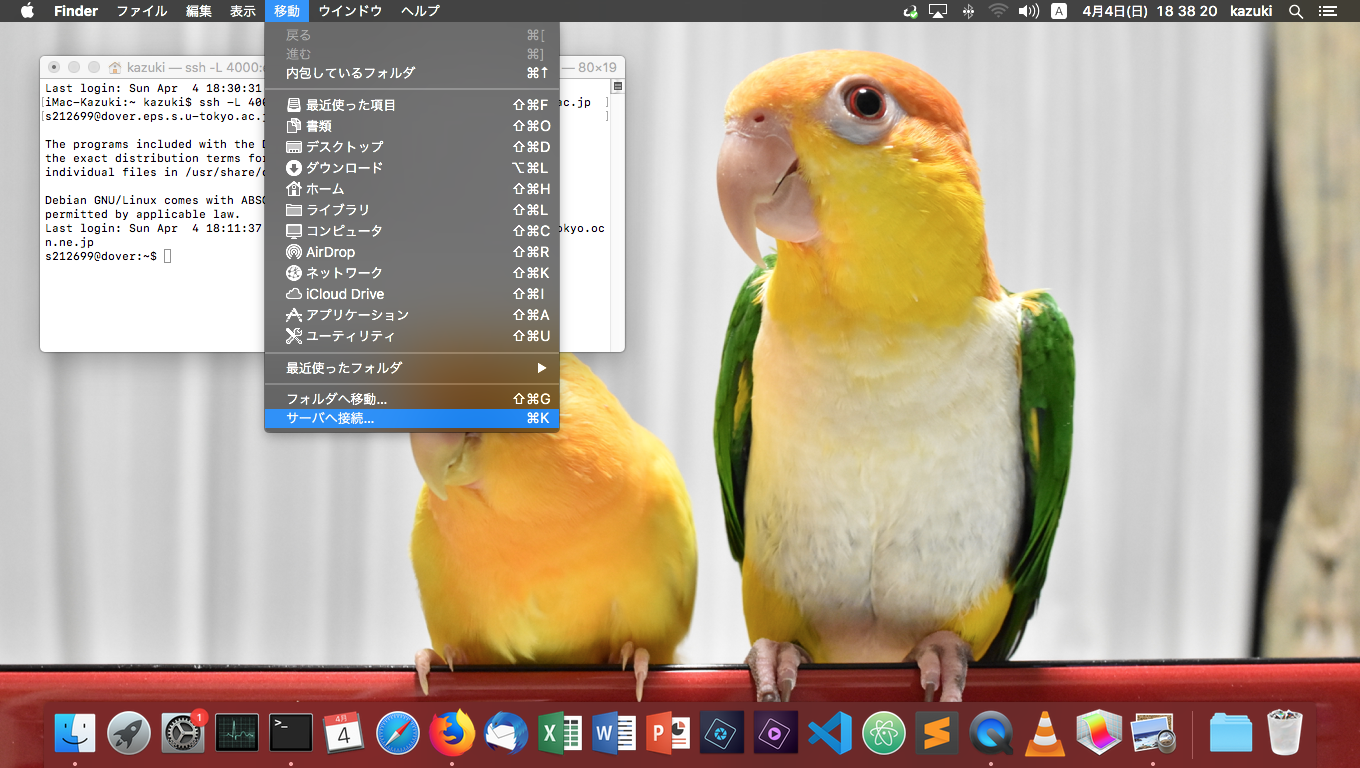
\includegraphics[height=7.5cm,pagebox=cropbox,clip]{fig/VNCMac2.png}
  \end{figure}
  \item 「vnc://localhost:4000」と入力し、接続をクリックします。
  \begin{figure}[H]
    \centering
    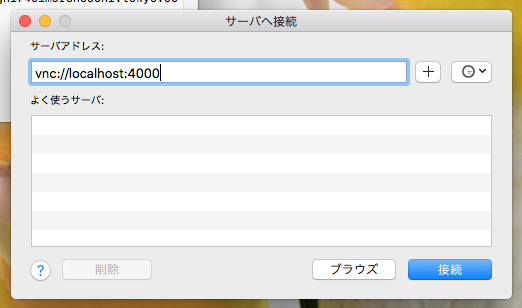
\includegraphics[height=6cm,pagebox=cropbox,clip]{fig/VNCMac3.png}
  \end{figure}
  \item 自分のアカウントとパスワードを入力します。
  \begin{figure}[H]
    \centering
    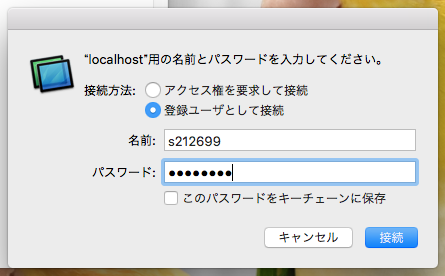
\includegraphics[height=5cm,pagebox=cropbox,clip]{fig/VNCMac4.png}
  \end{figure}
  このようなメッセージが表示された場合は、「自分のアカウントでログイン」を選択します。
  \begin{figure}[H]
    \centering
    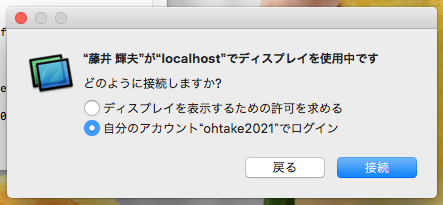
\includegraphics[height=4cm,pagebox=cropbox,clip]{fig/VNCMac5.png}
  \end{figure}
  \item eduのデスクトップが表示され、操作できます。
  \begin{figure}[H]
    \centering
    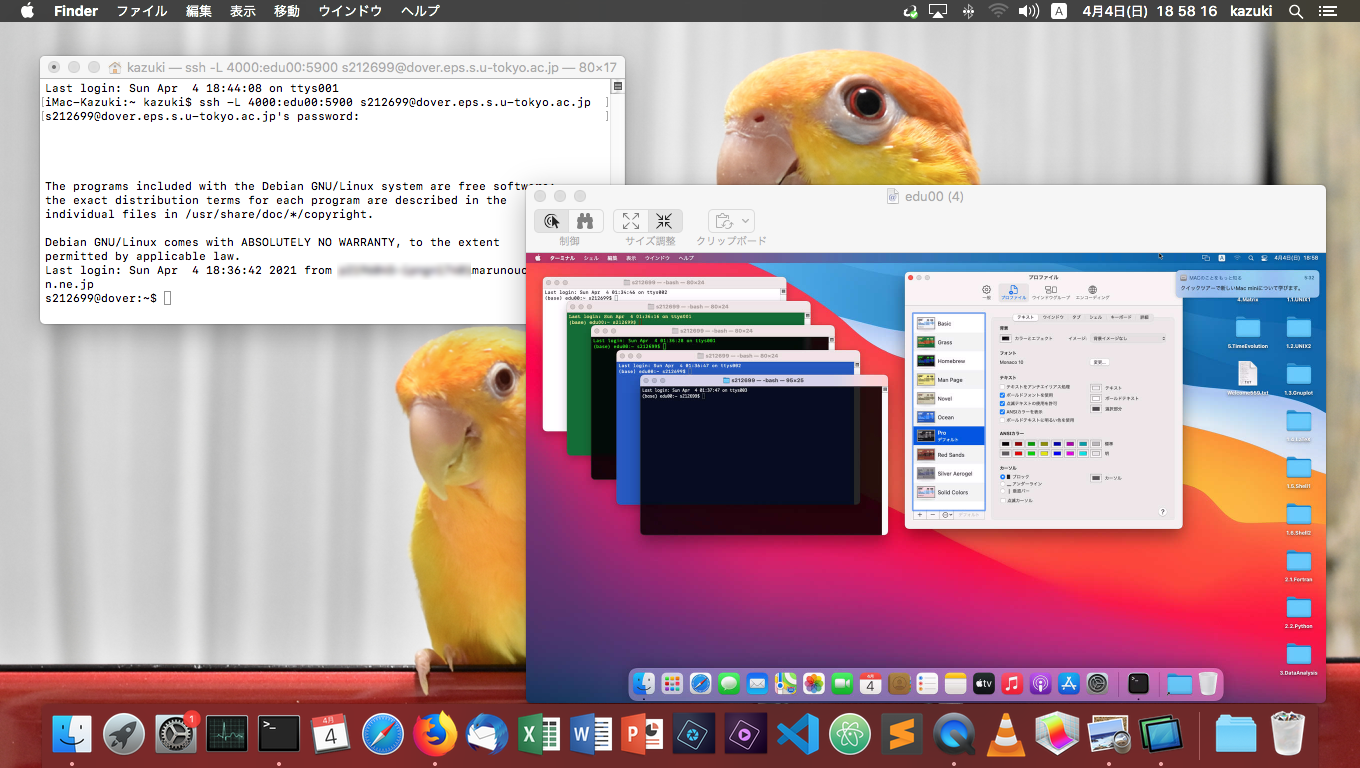
\includegraphics[height=7.5cm,pagebox=cropbox,clip]{fig/VNCMac6ed.png}
  \end{figure}
\end{enumerate}

\subsection{バックアップ}
毎週土曜日に,sakuraでは\verb|/home1|, \verb|/home2|のデータを\verb|/home1_backup|, \verb|/home2_backup|にそれぞれバックアップしています.
誤って大事なデータを消してしまった時にはsakuraにデータを取りに行きましょう.
ただし,土曜日を挟んでいない場合,バックアップはありません.あきらめてください.

データの回収の仕方は,まずsshでsakuraに入ります.
\begin{verbatim}
$ ssh sakura
\end{verbatim}
次に,\verb|/home1_backup/s2326??| に移動してください.
\begin{verbatim}
$ cd /home1_backup/s2326??/
\end{verbatim}
ここにバックアップのデータが保存されています.
お目当てのデータ(この例ではexample.txt)が見つかったら,それをsakura内の\verb|/home1/s2326??| にコピーすれば完了です.
\begin{verbatim}
$ cp /home1_backup/s2326??/example.txt /home1/s2326??/
\end{verbatim}
NFSによってデータが同期されているので,edu端末の中でも同じものを見ることができます.


\subsection{パスワードの変更方法}
パスワードを変更するのは少し複雑になります.というのも,edu,dover,www-geoph,asano  すべてに対して変更を適用する必要があるからです.

なお{\bf パスワードが分からなくなってしまった}時には後述の{\bf 計算機管理者(通称:admin210)}までご連絡ください.管理者が新しいパスワードを作成して再交付します.

\begin{table}[H]
  \centering
  \begin{tabular}{|l|l|l|l|} \hline
    場所 & & コマンド & 注意 \\ \hline
    559 & edu(01-35),sakura,asano & passwd & sshでsakuraにログインしてから行う \\ \hline
    559 & dover & passwd & sshでdoverにログインしてから行う  \\ \hline
    559 & www-geoph & passwd & sshでwww-geophにログインしてから行う  \\ \hline

  \end{tabular}
\end{table}
edu(Mac)では,システム環境設定→ユーザとグループ→パスワードを変更\ でもパスワードを変更できます.

\subsection{admin210(計算機管理者)}
geophネットワークは,{\bf 学生中心のボランティアスタッフ(admin210)}がネットワークとシステムの管理をしています.
このような管理体制は,学生ですべての管理を行わなければならないため大変ではありますが,学生の希望を通しやすいなど融通が利きます.
現時点でのUNIXやネットワークに関する知識の有無は問いませんので,興味のある人は積極的に参加してください.
参加希望者の連絡をお待ちしております.
admin210の連絡先は,\verb|admin210@eps.s.u-tokyo.ac.jp|です.
計算機に関する質問・要望・苦情なども遠慮なくどうぞ.プリンターのトナーが切れたとか用紙が足りないなどの相談も受け付けています.

特に,計算機に関して何か不具合を発見した場合(電源が点かない等)には必ず連絡するようにしてください.よろしくお願いします.

% \section{補遺}


\subsection{www-geophにファイルをアップロードする}
{\bf www-geoph}は地物演習室におけるWebサーバとして働いています.
演習室の中では,唯一doverを介さずに外部とやり取りができるマシンです.
ここにファイルを置いておくことによって,Web上でそのファイルを参照できるようにできます.

利用方法は,以下の通りです.
\begin{itemize}
\item sshでwww-geophにログインする

\verb| $ ssh www-geoph| 

\item ホームディレクトリ(ログイン時にいる場所)の中に\verb|public_html|というディレクトリを作る

参考:ディレクトリ作成方法(今いるディレクトリの中にtestという名前のディレクトリを作りたいとき)

\verb| $ mkdir test| (mkdirコマンドは次回以降詳しく学んでいきます)

\item Web上にアップしたいファイルをこのディレクトリ(\verb|public_html|)にscpでコピーすればOKです.

\verb| $ scp kadai2.txt www-geoph:test| (ssh・scpコマンドは次回以降詳しく学んでいきます)

例えばreport.pdfというファイルを転送した場合は
\url{http://www-geoph.eps.s.u-tokyo.ac.jp/~s2326??/report.pdf}
というURLでファイルがWeb上から見られるようになります.
シケプリをアップする時などに使うと便利かも知れません.
\end{itemize}

% \section{課題その2}
% \url{http://www-geoph.eps.s.u-tokyo.ac.jp/~s2326??/kadai/index.html}に何かしら文章なり単語なり絵なりを表示してください.
% 内容は問いませんが,外部(不特定多数)の人間からも見ることができるということは頭に入れておいてください.
% 基本的にはファイルが見つからないエラー「{\bf 404 Not Found}」にさえならなければOKです.
% できたと思ったらブラウザから見たりして,ちゃんと表示されているか確認してください.
% % 期限は,来週\textbf{2018年4月15日(月)13時(JST)}までとします.

\vspace{1em}

補足: wwwサーバのコンピュータは,アドレスにファイル名の指定がない場合「index.html」を探す仕組みになっており,
ホームページへのアクセスがあれば「index.html」のファイルを自動的にトップページとして認識し,そのデータを渡してくれます.
つまり,末尾のindex.htmlまでアドレスを入力しなくとも\url{http://www-geoph.eps.s.u-tokyo.ac.jp/~s2326??/kadai/}とさえ入力すればindex.htmlの中身が表示されます. 
試しに\url{http://www-geoph.eps.s.u-tokyo.ac.jp/~indy/kadai}
 (もしくは\url{http://www-geoph.eps.s.u-tokyo.ac.jp/~indy/kadai/index.html})と入力してみてください.
 下の画像のような画面が表示されるはずです.
\begin{figure}[htbp]
 \begin{center}
  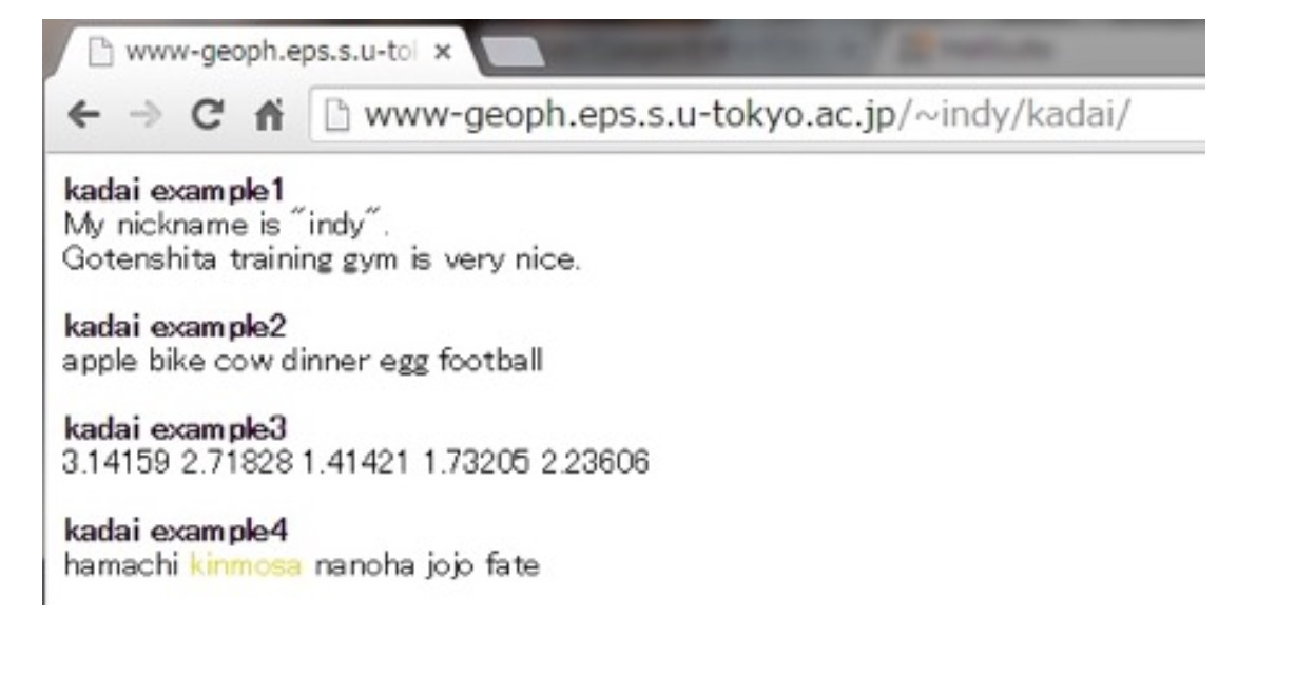
\includegraphics[width=90mm,pagebox=cropbox,clip]{fig/2.pdf}
 \end{center}
 \label{fig:one}
\end{figure}

このWebページのコンテンツは www-geoph の indy さんのホームディレクトリの中,\verb|~/public_html/kadai/index.html|に記載されています.どうすれば良いか分からない方は,この例を参考に考えてみると良いかもしれません.
\begin{center}
 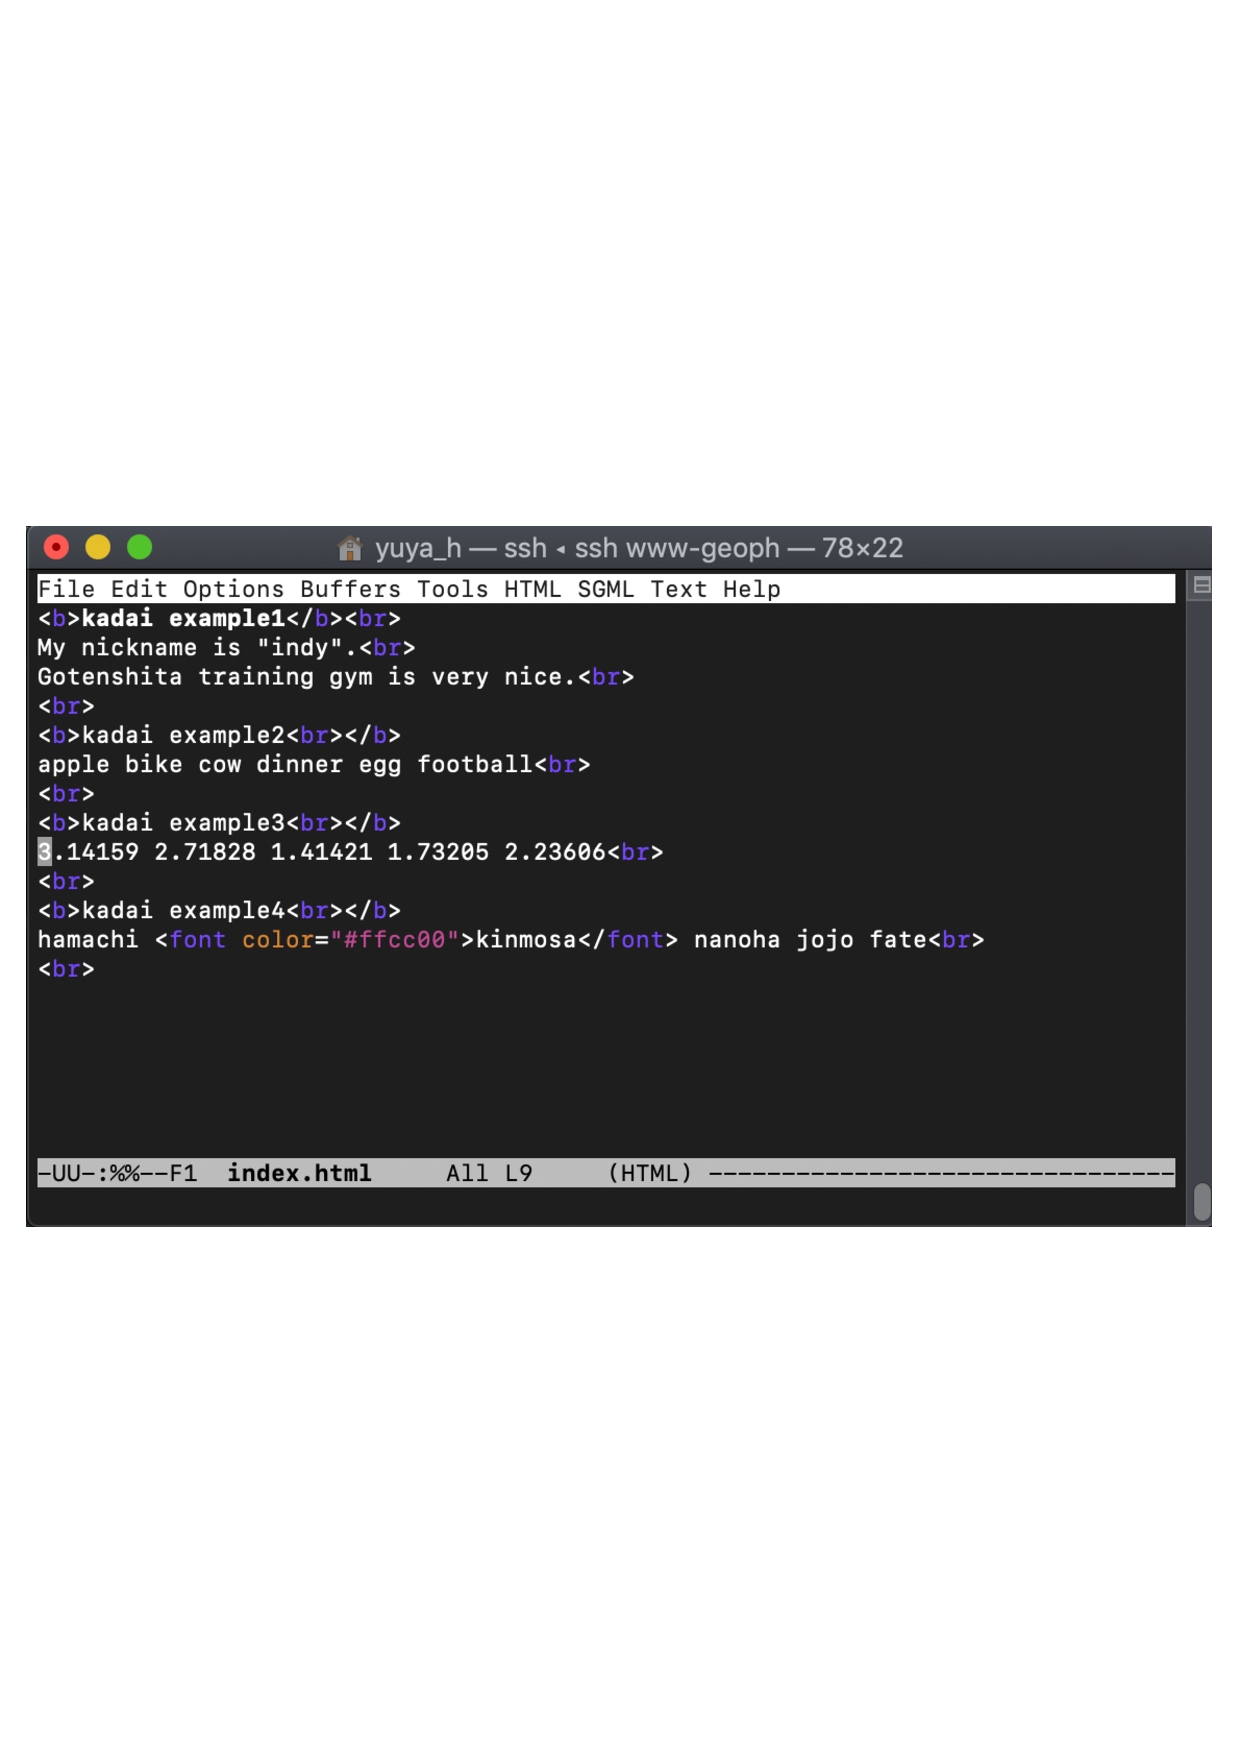
\includegraphics[width=90mm,pagebox=cropbox,clip]{fig/indy.pdf}
\end{center}
\end{document}